%%
%%  Hauptdatei
%%
%%  Projekt: Bachelorthesis 
%%  Autor:   Tobias Busch
%%  Status:  
%%  Datum:   28022017we
%%
%===================================================================
%% P R � A M B E L
%-------------------------------------------------------------------
%
%%==========================================================================================
%%
%% This is file 'FBMStyle.tex'  v 1.0
%% see also file 'FBMStyle_develop.tex
%%
%% Beta-Version eines Styles von Michael Arnemann
%% basieren auf einem Muster von Uwe Kappler 
%%
%% 2015-03-22 
%%========================================================================================== 
\documentclass[
        final,                % wenn es denn fertig ist.. 
        11pt,                 % Schriftgr��e (10pt, 11pt, 12pt) 11:pala:ok, 
        twoside,              % oneside, twoside
        numbers=noenddot,     % Kapitelnummer ohne . am Ende
        headings=normal,       % Groesse der Ueberschrift (bigheadings, normalheadings, 
        parskip=half,          % Europ�ischer Satz mit Abstand zwischen Abs�tzen
        index=totoc,             % Index ins Verzeichnis einf�gen	*** pr�fen     
%        headsepline,          % Strich unter Kopfzeile
        headinclude,          % Kopfzeile bei Satzspiegel bereucksichtigen
        DIV15,                % mit palatino 11pt oder CM 12
        BCOR14mm]             % Binderand    %1mm, f�r Klebebindung % 14mm dann etwa gleichm��ig
   {scrbook}                  % Dokumenttyp // f�r Dipomarbeiten, Diss
%----------------------------------------------------------------------------------------
%  PACKAGES
%----------------------------------------------------------------------------------------
\typearea                  % nach der Schrift
        [current]          % Heftrand BCOR oben definiert
%        {calc}             % DIV neu berechnen aus package 
        {last}             % DIV letzte aus Definition zuvor

\usepackage{lmodern}          % empfohlen anstatt CM Fonts, nur so korrekte Darstellung mit CM
%\usepackage{mathptmx}
%\fontfamily{ptm}\selectfont  %times

%\usepackage{helvet}
%\fontfamily{phv}\selectfont  %helvetica

\setkomafont{footnote}{\normalsize}                     % Marke und Text einer Fu�note
\usepackage{scrpage2}         % Package laden  

\usepackage[T1]{fontenc}      % T1-encoded fonts: auch W�rter mit Umlauten trennen
\usepackage[T1]{url}          % much like \verb allow line breaks for paths and URLs
\usepackage[latin1]{inputenc} % Deutsche Umlaute: Eingabe nach ISO 8859-1 (Latin1)

\usepackage{epsfig,xspace}    % PS Bilder
\usepackage{graphicx,color}   % JPEG und PNG 
                              % http://en.wikibooks.org/wiki/LaTeX/Colors  
\usepackage{subfigure}	      % Mehrere Bilder in einem mit ver. Bildunterschriften
\usepackage{wrapfig}	        % Text um Bild

\usepackage[ngerman]{babel}   % Neue deutsche Rechtschreibung  120412ar
%\usepackage[babel,german=guillemets]{csquotes} % f�r quotes
\usepackage[babel,german=quotes]{csquotes} % f�r quotes

%tools}             % enth�lt: afterpage, array, bm, calc, dcolumn, delarray, enumerate, fileerr, fontsmpl, ftnright, hhline, indentfirst, layout, longtable, multicol, rawfonts, showkeys, somedefs, tabularx, theorem, trace, varioref, verbatim, xr, and xspace.

\usepackage{latexsym}         % Sonderzeichen  f�r ??
\usepackage{pifont}           % dito
\usepackage{array}            % f�r aufw�ndigere Tabellen
\usepackage{longtable}        % seiten�bergreifende Tabellen passt zu KOMA
\usepackage{multicol}         % Mehrspaltiger Satz

\usepackage{makeidx}          % f�r Index-Erstellung 
%\usepackage{listings}         % f�r Latex Quelltext
%\usepackage{textcomp}         % for upright mu (\textmu)
\usepackage[fleqn]{amsmath}
\usepackage{amssymb}
\usepackage{eqnarray}	        % nummerierte und unnummerierte Gleichungen/systeme
\usepackage{ifthen}
\usepackage{fancybox}         % f�r schattierte ovale Boxen etc. geht nicht mit Miktex 5 060614ar
\usepackage{lscape}           % f�r landscape
\usepackage[normalem]{ulem}   % Unterstreichen und durchstreichen  Probleme mit bibtex
\usepackage{ziffer}           % Komma in math. Umgebung ohne folgendes Leerzeichen
\usepackage{cancel}           % K�rzen in Br�chen 

\usepackage[plainpages=false,pdfpagelabels]{hyperref}         
%
%% **** END OF CLASS MStyle ****
%


%\usepackage[ngerman]{babel}
%\usepackage[latin1]{inputenc}
%\usepackage[utf8]{inputenc}

\usepackage{esvect} %Vektorpfeile
\usepackage{graphicx,subfigure} % zwei Grafiken nebeneinander
\usepackage{todonotes}
\usepackage{booktabs}
\usepackage{multirow}
\usepackage{float}
\usepackage[latin1]{inputenc}

\usepackage{listings}       %benutzte packages S.W.
\renewcommand{\labelitemii}{\small\circ}%%----------------------------------------------------------------------
%% pdf-setup 060830ar
%%----------------------------------------------------------------------
%
%
\hypersetup{%
  %backref,%
  pdftitle    = {Richtlinien zur Durchf�hrung von Abschlussarbeiten},
  pdfsubject  = {Fakult�t f�r Maschinenbau und Mechatronik},
  pdfauthor   = {Prof. Dr.-Ing. M. Arnemann},
  pdfkeywords = {Richtlinie, Abschlussarbeit, Bericht},
%  pdfcreator  = {Adobe-Acrobat-Distiller},
%  pdfproducer = {LaTeX with hyperref und thumbpdf},
  pdfpagemode  = UseThumbs, % Anzeige Piktogramme
  bookmarksopen = true,     % Anzeige aller Ebenen
  bookmarksnumbered = true, % Anzeige Abschnittsnummern  
  pdfstartpage = {1}        % Startseite, hilfreich mit pdf
 }
% 

\hypersetup{%
%  pagebackref,
  bookmarksnumbered,
%  backref,
%  bookmarks,
%  breaklinks,
%  linktocpage,
%
%alternative Farbwahl
%  colorlinks  = true,
%  linkcolor   = blue,
%  urlcolor    = blue,
%  tocdepth     = 3            
}
             
%%
%% wenn f�r alles die gleiche Farbe ..
%%
%\definecolor{LinkColor}{rgb}{0,0,0.5} %duckelblau
%\definecolor{LinkColor}{rgb}{0,0,1} %blau
%\definecolor{LinkColor}{rgb}{0.5,0,0} % dunkelrot bis braun
%\definecolor{LinkColor}{rgb}{1,0,0} % rot
%\definecolor{LinkColor}{rgb}{0.7,0,0} % kr�ftig rot
%\definecolor{LinkColor}{rgb}{1,1,1} % wei�
\definecolor{LinkColor}{rgb}{0,0,0} % wei�
\hypersetup{%
  colorlinks=true,%
	linkcolor=LinkColor,%
	citecolor=LinkColor,%
	filecolor=LinkColor,%
	menucolor=LinkColor,%
%	pagecolor=LinkColor,%  gibt es nicht mehr
	urlcolor=LinkColor
}

%
% Makros       
% 120409ar
% 
%%=============================================================================
%% Abk�rzungen (Abteilung "Faulheit")
%%=============================================================================
%
% --- Gleichungen 
% Syntax: \beq{NAME DER GLEICHUNG} 
%         \eeq
% Referenz: \ref{eqt:NAME DER GLEICHUNG}
%
% begin
\newcommand{\beq}[1]
           {
            \begin{equation}
            \label{#1}
           }
% end
\newcommand{\eeq}
           {
             \end{equation}
           }
\newcommand{\ba}{\begin{array}}
\newcommand{\ea}{\end{array}}

\newcommand{\bdm}{\begin{displaymath}}
\newcommand{\edm}{\end{displaymath}}
	   
% --- Itemize 
\newcommand{\bi}{\begin{itemize}}
\newcommand{\ei}{\end{itemize}}

% --- Enumerate
\newcommand{\be}{\begin{enumerate}}
\newcommand{\ee}{\end{enumerate}}

% ---
\newcommand{\bd}{\begin{description}}
\newcommand{\ed}{\end{description}}

%R�misches Zahlen
\newcommand{\RNum}[1]{\uppercase\expandafter{\romannumeral #1\relax}}

% Fussnoten
% Syntax: \fn legt fest, wo das Fu�notenzeichen steht
%         \fnt{FUSSNOTENTEXT} legt den Text fest
\newcommand{\fn}{\footnotemark}
\newcommand{\fnt}[1]{\footnotetext{#1}}

\newcommand{\s}{\scriptscriptstyle}
\newcommand{\D}{\displaystyle}

\newcommand{\bff}[1]{\noindent {\textbf{#1}}}

\newcommand{\ol}{\ddot{O}l}
\newcommand{\p}{\partial}
\newcommand{\Dp}{\Delta p}
\newcommand{\te}{$\vartheta$}             % theta
\newcommand{\cT}{\vartheta}               %      Celsiustemperatur muss erhalten bleiben
\newcommand{\Ct}{\vartheta}               %var   Celsiustemperatur kann evtl in t ge�ndert werden

\newcommand{\R}{{\em\bf R}}               % Universelle Gaskonstante fett
\newcommand{\C}{$^\circ$C}                % Grad Celsius
%\newcommand{\C}{~\textcentigrade{}}                % Grad Celsius
%\newcommand{\CC}{^\circ\mbox{C}}                % Grad Celsius
\newcommand{\CC}{\,^\circ\mathrm{C}}                % Grad Celsius
\newcommand{\CCe}{^\circ\mathrm{C}}                % Grad Celsius
\newcommand{\mue}{\textmu}
\renewcommand{\d}{\partial\mspace{2mu}}   % partielles Diff. Zeichen 
\newcommand{\td}{\,\mathrm{d}}           	% totales Diff (d, nicht kursiv)
\newcommand{\ddt}[1]{\frac{\td #1}{\td t}}% zweifach 

%% ggfl. umschreiben mit \text{}
\newcommand{\idx}[1]{_\mathrm{#1}}        % nicht kursiver Index in Gleichungen geht nur mit Umlauten wie "a
\newcommand{\idxi}[2]{_{\mathrm{#1,}{#2}}}% nicht kursiver Index in Gleichungen geht nur mit Index 
\newcommand{\idy}[1]{^\mathrm{#1}}        % nicht kursiver Index in Gleichungen geht nur mit Umlauten wie "a


\newcommand{\bul}{$\bullet$}              % Mark in Tabs
\newcommand{\Q}{$\bullet$}                % mark2 in Tabs
\newcommand{\mc}{\multicolumn}

%\def\dbar{{\mathchar'26\mkern-12mu d}}  %(The space after the \mu" is optional but is added f
\def\dbar{{\mathchar'26\mkern-11mu\mathrm{d}}}  %130102ar hier f�r lmodern,  achtung passt nich bei jedem Font !
%\def\dbar{{\mathchar'26\mkern-9mu\mathrm{d}}}  %130102ar hier f�r times !

\def\bzw{bzw.\ }
\def\bspw{bspw.\ }
\def\ca{ca. }
\def\dh{d.\,h.\ }
\def\etc{etc.\ }
\def\evtl{evtl. }
\def\ggf{ggf.\ }
\def\inkl{inkl.\ }
\def\o�{o.\,�.\ }
\def\og{o.\,g.\ }
\def\so{s.\,o.}
\def\su{s.\,u.}
\def\ua{u.\,a.\ }
\def\zB{z.\,B.\ }
\def\zT{z.\,T.\ }

%% Spezialit�ten f�r klimatechnik
\def\mp{\dot{m}}
\def\m.{\dot{m}} % geht
\def\V.{\dot{V}} % geht
\def\pws{p\idx{W}\idy{s}(T)} % geht

\newcommand{\name}[1]{\textsc{#1}}  % f�r Firmen, Autoren

\def\Re{\mathin{Re}}
\def\Nu{\mathin{Nu}}
\def\Pr{\mathin{Pr}}

%%
%%
%%
\newcommand{\uu}[1]{\emph{#1}}  %Texthervorhebung
%%
%% Refrenzen -------------------------------------------------
%%
%\newcommand{\RefTab}[1]{$\underline{\mbox{Tab.~\ref{#1}}}$}   % 1. Tabellenref. im Text
%\newcommand{\RefFig}[1]{$\underline{\mbox{Abb.~\ref{#1}}}$}   % 1. Bildref.
%\newcommand{\RefTab}[1]{\textbf{Tabelle~\ref{#1}}}             % 1. Tabellenref. im Text
\newcommand{\RefTab}[1]{{\small \color{LinkColor}$\blacktriangleright${Tabelle~\ref{#1}}}} % 1.

%\newcommand{\RefFig}[1]{{\color{blue}$\blacktriangleright$\textbf{Bild~\ref{#1}}}} % 1.
%\newcommand{\RefFig}[1]{{\color{LinkColor}$\blacktriangleright$\textbf{Bild~\ref{#1}}}} % 1.
%\newcommand{\RefFig}[1]{\textbf{Bild~\ref{#1}}}                % 1. Bildref.
%\newcommand{\RefFig}[1]{{\color{LinkColor}$\blacktriangleright${Bild~\ref{#1}}}} % 1.
\newcommand{\RefFig}[1]{{\small \color{LinkColor}$\blacktriangleright${Bild~\ref{#1}}}} % 1.

%\newcommand{\RefTabc}[1]{Tabelle~\ref{#1}}                     % 2. Tabellenref. im Text
\newcommand{\RefTabc}[1]{{\small Tabelle~\ref{#1}}}             % 2.
%\newcommand{\RefFigc}[1]{Bild~\ref{#1}}                        % 2. Bildref.
\newcommand{\RefFigc}[1]{{\small Bild~\ref{#1}}}                % 2. Bildref.

\newcommand{\RefEq}[1]{\mbox{Gl.~(\ref{#1})}}                  % Gleichungen

% \autoref{label} % Erzeugt link inkl dem Wort Abbbildung
% \nameref{label} % Kapiteltext
 
%
%
%
\newcommand{\ZmE}[2]{$#1$~{#2}}                                % Zahl:#1 mit Einheiten#2 #3
%\newcommand{\zme}[2]{$#1$~{#2}}                               % Zahl:#1 mit Einheiten#2 #3
\newcommand{\zme}[2]{#1~\mbox{#2}}                             % Zahl:#1 mit Einheiten#2 #3
\newcommand{\EH}[1]{#1}                                        %  Einheiten
\newcommand{\B}[1]{\mbox{#1}}

%-------------------------------------------------------------
\newfont{\ssf}{cmss10 scaled 1000}
\newfont{\ssb}{cmssbx10 scaled 1000}
\newcommand{\cf}{\ssf}                 % CaptionFonts: in Bildunter- ,Tab?berschriften
\newcommand{\rf}{\em}                  % RefFonts    : Kennzeichnung von Referenzen im Text
\newcommand{\eng}{\tt}                 % englische Begriffe im deutschen Text 

% Hinweis
% Syntax: \oops{�BERSCHRIFT}{TEXT}
%        : nach �berschtift wird automatisch eingef�gt
\newcommand{\oops}[2]{\begin{quote}\textbf{#1}:\\ {#2} \end{quote} }

%---------------------------------------------------------------
% Bildunter- und Tabellen�berschriften
%---------------------------------------------------------------
% z.B. andere Schrift, oder auch Schriftform und andere Abk�rzung
%
% alternaiv : "Abbildungen" lassen und
%  Zeilenumbruch bei Bildbeschreibungen einf�hren \setcapindent{1em}
%
% bessere Methoden: siehe Komaskript
\def\figurename{Bild}          % oder: Bild z.B. {\bfseries Abb.}
%\def\tablename{Tab.}          % oder: z.B. Tafel, Tab.

\renewcommand*{\captionformat}{.~} % DIN l�sst gr�ssen
%\addtokomafont{caption}{\sffamily\small\raggedright}  % kleinere Schrift, linksb�ndig
\addtokomafont{caption}{\sffamily\small}  % kleinere Schrift
%\setkomafont{descriptionlabel}{\sffamily\small}
\setkomafont{captionlabel}{\sffamily\bfseries}
\setcaphanging
\setcapindent{0em}             % kein Einzug

%---------------------------------------------------------------
% Kommentare 
\newcommand{\Kommentar}[1]{{\em #1}} 


% Verstecktes
% Alles innerhalb von \Hide{} oder \ignore{}
% wird von LaTeX komplett ignoriert (wie ein Kommentar)
%------------------------
% methode 1
\newcommand{\Hide}[1]{}
\let\ignore\Hide
\newcommand{\HideB}[1]{}
\let\ignore\HideB

%--eigner Befehl, l�sst sich besser modifizieren
%
\newcommand{\mynewpage}{\newpage}
\newcommand{\myclearpage}{\clearpage}


%\usepackage{tabularx} % automatische Spaltenbreite 
\newcolumntype{L}[1]{>{\raggedright\arraybackslash}p{#1}}
\newcolumntype{C}[1]{>{\centering\arraybackslash}p{#1}}
\newcolumntype{R}[1]{>{\raggedleft\arraybackslash}p{#1}}

\newcommand{\LCIRC}[1]{{\large\textcircled{\normalsize \texttt{#1}}}}
\newcommand{\NCIRC}[1]{\textcircled{ {\small \texttt{#1}} } }


%Umgebung
\def\d@nger{\marginpar[\hfill\dbend]{\dbend\hfill}}
\newenvironment{danger}{\medskip\hspace{0pt}\d@nger}{\medskip}

% for multicolumn
\newcommand{\cg}{\centering}  %120409ar

%%%%%%%%%%%%%%%%%%%%%%%%%%%%%%%%%%%%%%%%%%%%%%%%%%%%%%%%%%%%%%%%%%%%%%%%%%%%%%%%%%%%%%%%%%%%%%%%%%%%%%%%%%%%%%%%%%%%%%%%%%%%%%%%%%%%%%%%%%%%%
%%%%%%%%%%%%%%%%%%%%%%%%%%%%%%%%%%%%%%%%%%%%%%%%%%%%%%%%%%%%%%%%%%%%%%%%%%%%%%%%%%%%%%%%%

\def\Sum{\scalebox{0.7}{$\sum$}}
\def\IntIm{\scalebox{1.2}{$I�}}
         % Macros lagen
%-----------------------------------------------------------------
% Beschriftung des Titelblatts - Vorderseite
% 061218ar
%-------------------------------------------------------------------
%
\usepackage{titlepage-HsKa/HsKAtitle11}

\department{Fakult�t f�r Maschinenbau und Mechatronik}

\title{Erkennen von Fahrbahnen, Fahrbahnmarkierungen, Hindernissen   und Verkehrszeichen mittels Bildverarbeitung   
       \vspace*{1em}                        
      } 

\thesistype{Masterarbeit (M.Sc.)}  % *Bachelorarbeit B.Eng.  *Masterthesis (M.Sc.)      
\thesisno{*B 15/1000}          % siehe Anmeldeformular     

\author{Tobias Busch}
\BDate{26. 02. 1993}
\BLocation{Rastatt}
\matno{60059}

\companyname{Hochschule Karlsruhe}
\tutor{Referent: Prof. Dr.-Ing. Ferdinand Olawsky}{Korreferent: Dipl.-Ing. (FH) Beck Bernhard}
\location{Karlsruhe}
\duration{1. 09. 2019  bis  2. 03. 2020}

%\restrictionnotice{*S P E R R V E R M E R K}      
\restrictionnotice{*** V E R T R A U L I C H ***}      
%%
% Bemerkung auf der R�ckseite, wenn zweiseitig
%
\Schriftsatz{%
    
    }%
    
%         % Titeldefinition, kann so nicht genutzt werden


\makeindex

%===================================================================
% B E G I N N  D E S  D O K U M E N T S
%
%% Hier kommen die einzelnen Kapitel, die jeweils in einem eigenen
%% Folder stehen. Dateiendung MUSS .tex sein. Wird hier nicht angegeben. 
%% W I C H T I G : Pfade in Unix-Syntax d.h.:
%% 0010/chapter und NICHT 0010\chapter !!!
%% ALLE PFADE RELATIV ZU DIESER DATEI!!
%-------------------------------------------------------------------
\begin{document}

\pagestyle{scrheadings}            % Kopf- und Fusszeilen
\clearscrheadfoot                  % Alles auf "" setzen
\pagestyle{empty}
   

% Titelblatt erzeugen
%%
%%  Pagestyle f�r Pre
%%  061218ar
%==============================================================================
%
\pagestyle{scrheadings}            % Kopf- und Fusszeilen
\clearscrheadfoot                  % Alles auf "" setzen
\setcounter{page}{100}             % anpassen: wenn 1-seitig  dann 2     
\pagenumbering{roman}
\lehead{\pagemark \hspace*{2em} \headmark}
\rohead{\headmark \hspace*{2em} \pagemark}
\maketitle  %erzeugt 1 --> kein Fehler



%%
%% Erkl�rung und Sperrvermerk
%%
%% Vorsicht beim Entfernen von \\ und Leerzeilen
%%
%% Sperrvermerk nur wenn zwingend !
%%------------------------------------------------------------------------
%
\setcounter{page}{3}       % anpassen: wenn 1 Seitig  dannn 2     
\pagestyle{scrheadings}    % Kopf- und Fusszeilen

\chapter*{}
\centerline{\Large \textsf{\textbf{Erkl�rung}}} \label{Erklaerung}%\\
\vspace*{2ex}
%
Ich versichere hiermit wahrheitsgem��, die Abschlussarbeit selbstst�ndig angefertigt, alle benutzten Hilfsmittel vollst�ndig und genau angegeben und alles einzeln kenntlich gemacht zu haben, was aus Arbeiten anderer unver�ndert oder mit Ab�nderungen entnommen wurde.\\
\\
\\

\vspace*{4ex}
Karlsruhe, den \today \\

\vspace*{4ex} 
Unterschrift:\\


\vspace{2cm}

%--------------------------------------------------------------

%\raggedbottom
%\cleardoublepage
%**************************************************************




     % Hochschul-spezifisch
\let\cleardoublepage\clearpage
%%
%%  061115ar 
%%
%%=============================================================================
\pagestyle{scrheadings}            % Kopf- und Fusszeilen
%\section*{Danksagung}
\chapter*{} \label{Danksagung}
\centerline{\Large \textsf{\textbf{Danksagung}}} %\\
\vspace{2ex}
%
%
An dieser Stelle m�chte ich mich bei all denen bedanken, die mich bei der Erstellung dieser Masterarbeit unterst�tzt haben. Besonderer Dank geb�hrt meinem Betreuer, Herrn Prof. Dr.-Ing Ferdinand Olawsky, welcher mir diese Abschlussarbeit erm�glicht und mich bei Fragen und auftretenden Problemen stets motiviert unterst�tzt hat. 
Weiterer Dank gilt Herrn Dipl.-Ing. Bernhard Beck, an den ich mich bei fachspezifischen Fragen jederzeit wenden konnte. Abschlie�end m�chte ich meiner Familie und meinen Freunden f�r die Unterst�tzung w�hrend meines Studiums danken.



%\cleardoublepage
%\thispagestyle{empty}.
%\newpage
%-----------
%%
%%
%%
%\thispagestyle{empty}
%\clearscrheadfoot                  % Alles auf "" setzen
%------------------------------------------------------------------------------

\section*{Kurzfassung} \label{Kurzfassung}
Die vorliegende Arbeit besch\"aftigt sich mit den Herausforderungen des autonomen Fahrens nach den Anfoderungen des Carolo-Cups der TU-Braunschweig. Betrachtet wurde die Erkennung von Fahrbahnen, Fahrbahnmarkierungen, Hindernissen und Verkehrszeichen in Kamerabildern und das Bewerten von sicheren Fahrbahnbereichen. Zudem wurde die Simulation der Wettbewerbsbedingungen des Carolo-Cups behandelt.
Durch Auswahl einer geeigneten Entwicklungs- und Simulationsumgebung wurde ein Bildverarbeitungstestframework entwickelt. Verschiedene Verfahren von Bildverarbeitungsalgorithmen wurden implementiert und bewertet.
Zur Klassifikation von Geschwindigkeitsmarkierungen wurden drei verschiedene Machine-Learning-Ans\"atze evaluiert.
Das Ergebnis dieser Arbeit ist ein Bildverarbeitungssystem, das in einer Simulationen durch verschiedene implementierte Testszenarien evaluiert werden kann, um damit in kommenden Carolo-Cup-Wettbewerben erfolgreich anzutreten. 


 




\newpage

\section*{Abstract} \label{Abstract}

The work in hand deals with the challenges of autonomous driving after the requirements of the Carolo-Cup of the TU-Braunschweig. The recognition of lanes, lane markings, obstacles and traffic signs in camera images and the evaluation of safe lane areas were considered. Simulation of the competitive conditions of the Carolo-Cup were treated.
An image processing test framework was developed by selecting a suitable development and simulation environment. Various methods of image processing algorithms have been implemented and evaluated.
Three different machine learning approaches were evaluated to classify speed markers.
The result of this work is an image processing system that can be evaluated in a simulation using various implemented test scenarios in order to successfully compete in upcoming Carolo-Cup competitions.





















%\cleardoublepage% als Kurzfassung formuliert
%-----------
%%==============================================================
%
% Nomenklatur
%
%==============================================================
\chapter*{Nomenklatur}%
  \label{Nomenklatur}%
   % Die folgende Zeile erzwingt einen Eintag ins Inhaltsverz.
  \addcontentsline{toc}{chapter}{Nomenklatur}%
%-----------
\manualmark
\markright{Nomenklatur}
\markleft{Nomenklatur}
%\ohead[]{\headmark}
%\begin{longtable}{p{3cm} p{2cm} p{\textwidth}}  % ACHTUNG Breite
\begin{longtable}{p{0.15\textwidth} p{0.15\textwidth} p{0.55\textwidth}}  % ACHTUNG Breite 0.9
%-----------------------------------------------

\multicolumn{3}{l}{%
\textbf{\textsf{\large Abk�rzungen}}
}\\
%---------------------------------------------

API       & & Application Programming Interface\\
CAD       & & Computer-Aided Design\\
CNN       & & Convolutional Neural Network\\
cuDNN     & & NVIDIA CUDA Deep Neural Network library\\
FPS       & & Frames per second\\
GPU       & & Graphics Processing Unit\\
GUI       & & Graphical User Interface\\
IDE       & & Integrated Development Environment\\
KNN       & & K�nstliches Neuronales Netz\\
OGRE      & & Object-Oriented Graphics Rendering Engine\\
OSRF      & & Open Source Robotics Foundation\\
PNG       & & Portable Network Graphics\\
QR        & & Quick Response\\
RAM       & & Random Access Memory\\
ROS       & & Robot Operating System\\
ROI		  & & Region of Interest\\
SDF       & & Simulation Description Format\\
XML       & & Extensible Markup Language\\
 




\end{longtable}

%\cleardoublepage




















    % Formel und Abk�rzungsverzeichnis 
%
% Inhalt und Listen
%-----------------------------------------------------------------

\manualmark
\markright{Inhaltsverzeichnis}
\markleft{Inhaltsverzeichnis}
\tableofcontents                   % Inhaltsverzeichnis erzeugen
%\cleardoublepage


%\manualmark
%\markright{Tabellenverzeichnis}
%\markleft{ Tabellenverzeichnis}
%\listoftables                      % Tabellenverzeichnis
%      % Die folgende Zeile erzwingt einen Eintag ins Inhaltsverz.
%      \addcontentsline{toc}{chapter}{Tabellenverzeichnis}
%\cleardoublepage
%
\manualmark
\markright{Abbildungsverzeichnis}
\markleft{ Abbildungsverzeichnis}
\listoffigures                     % Abbildungsverzeichnis erzeugen
%      % Die folgende Zeile erzwingt einen Eintag ins Inhaltsverz.
%      \addcontentsline{toc}{chapter}{Abbildungsverzeichnis}


%\cleardoublepage





%==============================================================
%
% Nomenklatur
%
%==============================================================
\chapter*{Nomenklatur}%
  \label{Nomenklatur}%
   % Die folgende Zeile erzwingt einen Eintag ins Inhaltsverz.
  \addcontentsline{toc}{chapter}{Nomenklatur}%
%-----------
\manualmark
\markright{Nomenklatur}
\markleft{Nomenklatur}
%\ohead[]{\headmark}
%\begin{longtable}{p{3cm} p{2cm} p{\textwidth}}  % ACHTUNG Breite
\begin{longtable}{p{0.15\textwidth} p{0.15\textwidth} p{0.55\textwidth}}  % ACHTUNG Breite 0.9
%-----------------------------------------------

\multicolumn{3}{l}{%
\textbf{\textsf{\large Abk�rzungen}}
}\\
%---------------------------------------------

API       & & Application Programming Interface\\
CAD       & & Computer-Aided Design\\
CNN       & & Convolutional Neural Network\\
cuDNN     & & NVIDIA CUDA Deep Neural Network library\\
FPS       & & Frames per second\\
GPU       & & Graphics Processing Unit\\
GUI       & & Graphical User Interface\\
IDE       & & Integrated Development Environment\\
KNN       & & K�nstliches Neuronales Netz\\
OGRE      & & Object-Oriented Graphics Rendering Engine\\
OSRF      & & Open Source Robotics Foundation\\
PNG       & & Portable Network Graphics\\
QR        & & Quick Response\\
RAM       & & Random Access Memory\\
ROS       & & Robot Operating System\\
ROI		  & & Region of Interest\\
SDF       & & Simulation Description Format\\
XML       & & Extensible Markup Language\\
 




\end{longtable}

%\cleardoublepage





















%
%-------------------------------------------------------------------
%  Hauptteil
%-------------------------------------------------------------------
%
%%
%%  Pagestyle f�r Hauptteil
%%  061218ar
%=============================================================================
\automark[section]{chapter}
\clearscrheadfoot                  % Alles auf "" setzen
\pagestyle{scrheadings}            % Kopf- und Fusszeilen
\pagenumbering{arabic}
\setcounter{page}{1}
%
\lehead{\pagemark \hspace*{2em} \headmark}
\rohead{\headmark \hspace*{2em} \pagemark }
%
% alternativ
%
%\ohead[\pagemark]{\pagemark}
%\ihead[]{\headmark}
%\ifoot[Hochschule Karlsruhe - Fakult�t f�r Maschinebau und Mechantronik]{Diplomarbeit KOMA OMA}
%\ifoot[]{Diplomarbeit KOMA OMA}    % wennn es denn sein muss

%%  Kolumnentitel  %%%%%%%%%%%%%%%%%%%%%%%%%%%%%%%%%%%%%%%%%%%%%%%%%%%
%%  alternativ: von wiley 
%%
\clearscrheadings
\clearscrplain
\pagestyle{scrheadings}

\lehead[%
  \llap{%
    \pagemark
    \hspace{1mm}%
    \smash{\rule[-2.8mm]{1pt}{6mm}}%
    \hspace{2mm}%
  }%
]{%
  \llap{%
    \pagemark
    \hspace{1mm}%
    \smash{\rule[-2.8mm]{1pt}{6mm}}%
    \hspace{2mm}%
  }%
  {%
    \sffamily
    \itshape
    \selectfont
    \headmark
  }%
}

\rohead[%
  \rlap{%
    \hspace{2mm}%
    \smash{\rule[-2.8mm]{1pt}{6mm}}%
    \hspace{1mm}%
    \pagemark
  }%
]{%
  {%
      \sffamily
    \itshape
    \selectfont
    \headmark
  }%
  \rlap{%
    \hspace{2mm}%
    \smash{\rule[-2.8mm]{1pt}{6mm}}%
    \hspace{1mm}%
    \pagemark
  }%
}

\renewcommand\pnumfont{%
  \sffamily%
  \bfseries
  \upshape
%  \fontsize{8}{12}%
  \fontsize{10}{12}%
  \selectfont
}

\renewcommand\headfont{%
  \sffamily%
  \itshape
%  \fontsize{8.5}{12}%
  \fontsize{10}{12}%
  \selectfont
}
%

% Beginn Literaturverzeichnis 
% 
%\ Stil f�r das Literaturverzeichnis ausw�hlen, alle Stile nach Din 1505  -------------------   %
%\bibliographystyle{gerplain} 
%\bibliographystyle{unsrt} 
%\bibliographystyle{plaindin} %alphabetisch 
%\bibliographystyle{abbrvdin} %wie plaindin, nur abgek�rtze Scheibweise

%\bibliographystyle{natdin}   %statt[1] steht z.B. [Kohm(2006)] vor dem entspr. Eintrag im Verzeichnis


\bibliographystyle{unsrtdin} % 1505 in der Reihenfolge wie im Text
%\bibliographystyle{alphadin} %alphabetische Reihenfolge, statt [1] steht z.B.[Koh]vor dem entspr. Eintrag im




%
%% Kapitel: Grundlagen
%%======================================================================


\chapter{Einleitung}
\label{cha:Einleitung} \index{Einleitung}


%-----------------------------------------------------------------------
\section{Aufgabenstellung}
\label{sec:Aufgabenstellung}\index{Aufgabenstellung}



\section{Gliederung}
\label{sec:Gliederung}\index{Gliederung}




%-----------------------------------------------------------------------

     % Der Teil Einleitung
%
%% Kapitel: Grundlagen
%%======================================================================


\chapter{Einf�hrung in die Programmierwerkzeuge}
\label{cha:Einf�hrung in die Programmierwerkzeuge} \index{Einf�hrung in die Programmierwerkzeuge}
%
%


%-----------------------------------------------------------------------


\section{Einf�hrung in die Funktionen der Stanard Template Library}
\label{sec:Einf�hrung in die Funktionen der Stanard Template Library}
Die Programmiersprache C++ ist eine Erweiterung von C und wurde ab 1979 von Bjarne Stroustrup entwickelt. Die M�glichkeit mit C++ objektorientierte Software zu entwickeln und somit Probleme in Klassen zu abstrahieren, erm�glicht eine einfachere Einarbeitung in den Programm-Code. Dies ist damit zu begr�nden das Menschen gewohnt sind in Objekten zu denken. 
Vor allem die Performanzvorteile beg�nstigen das Nutzen von C++ in der Bildverarbeitung, da die Sprache es erlaubt maschinennah zu programmieren und somit alle Leistungsgrenzen der Hardware voll auszunutzen.  
C++ ist eine Compilersprache. Die Performanz auf der Hardware ist deshalb auch abh�ngig von den verwendeten Optimierungsalgorithmen des genutzten Compilers. Der verwendete Compiler ist der auf dem Linux-Derivat Ubuntu 18.04 installierte GNU Compiler Collection kurz GCC. Der Programm dieser Arbeit ist mit der GCC-Version 7.4.0 entwickelt und kompiliert worden. Die Programmiersprache C++ entwickelt sich fortlaufend weiter, um mit der sich schnell ver�ndernden Computer-Technik Schritt zu halten. Der C++-11-Standard und die Features der Standard Template Library (STL) werden in der in dieser Arbeit entwickelten Software ausgiebig verwendet, deshalb werden im Folgenden die wichtigsten Features vorgestellt.


\subsection{auto}
\label{subsec:auto}
Der Platzhaltertyp-Bezeichner auto erm�glicht es, den zu deklarierenden Typ einer Variablen automatisch durch ihren Initialisierer abzuleiten. Daraus ergibt sich vor allem eine bessere Lesbarkeit des Codes. Dies ist vorallem bei Iteratoren der Fall.

\begin{lstlisting}
auto variable = 5;
\end{lstlisting}






\subsection{Vector-Container}
\label{subsec:Vector-Container}
Vektoren sind mit dynamischen Arrays identisch. Sie �ndern ihre Gr��e automatisch, wenn ein Element eingef�gt (push{\tiny\_}back) 
oder entfernt wird (erase). Vector ist ein Template und kann mit verschiedenen Datentypen wie zum Beispiel Variablen, Pointern oder ganzen Klassen deklariert werden.
Vektorelemente werden in einem zusammenh�ngen Speicher abgelegt, dadurch k�nnen sie mit Iteratoren durchlaufen werden. 

\begin{lstlisting}
vector<int> vec = {0, 1, 2, 3, 4};

vec.push_back(5);

vec.erase(vec.begin() + 5);
\end{lstlisting}

\subsection{Iterator}
\label{subsec:Iterator}
Iteratoren werden verwendet, um auf die Speicheradressen von STL-Containern zu verweisen und diese so zu durchlaufen. Sie verringern die Komplexit�t und Ausf�hrungszeit des Programms. 
\begin{lstlisting}
vector<int> vec = {0, 1, 2, 3, 4};

for(auto it = vec.begin(); it < vec.end(); it++)
{
	cout << it << endl;
}

for(auto it : vec){cout << it << endl;}
\end{lstlisting}


\subsection{Pair-Container}
\label{subsec:Pair-Container}
Pair wird verwendet, um zwei Werte miteinander zu kombinieren, deren Typ unterschiedlich sein kann. Pair bietet die M�glichkeit, zwei heterogene Objekte als eine Einheit zu speichern. Das erste Element wird als \"first\" und das zweite Element als \"second\" bezeichnet.Die Reihenfolge der Elemente ist fest definiert (first, second).
\begin{lstlisting}
pair<string,int> bild_merkmal;

bild_merkmal.first = "Mittellinie"

bild_merkmal.second = 42;

vector< pair<string,int> > bild_merkmale;

bild_merkmale.push_back(make_pair("Mittellinie",42)); 

\end{lstlisting}
\subsection{Map- und unordered Map-Container}
\label{subsec:Map- und unordered Map-Container}
Maps sind assoziative Container, in denen Elemente zugeordnet gespeichert werden. Jedes Element hat einen Schl�sselwert und einen zugeordneten Wert. Keine zwei zugeordneten Werte k�nnen denselben Schl�sselwert haben.
Der Map-Container sortiert dabei seine Elemente nach aufsteigender Reihenfolge w�hrend der unordered{\tiny\_}map Container dies nicht tut. Das Sortieren der Elemente kann Performanzvorteile bei der Suche von Elementen im Container erm�glichen. Es ben�tigt jedoch auch mehr Zeit beim Einf�gen oder l�schen der Elemente. Der Map-Container besitzt im schlechtesten Fall eine Zeitkomplexit�t von O(log(n)) und der Unordered{\tiny\_}map-Container eine Zeitkomplexit�t von O(n).
%https://hackernoon.com/what-does-the-time-complexity-o-log-n-actually-mean-45f94bb5bfbf
\begin{lstlisting}
map<string,int> bild_merkmale_anzahl;

bild_merkmale_anzahl.insert(make_pair("Mittellinien", 42)); 

bild_merkmale_anzahl.insert(make_pair("Parkfl�chen", 5)); 

bild_merkmale_anzahl.insert(make_pair("Au�enlinien", 2)); 

int anzahl_mittellinien = bild_merkmale_anzahl["Mittellinien"];

\end{lstlisting}

\subsection{Multimap- und unorderderd Multimap-Container}
\label{subsec:Multimap- und unorderderd Multimap-Container}
Multimap-Container sind assoziative Container, in denen Elemente gespeichert werden, die aus einer Kombination eines Schl�sselwerts und eines zugeordneten Werts in einer bestimmten Reihenfolge bestehen und in denen mehrere Elemente �ber denselben Schl�ssel verf�gen k�nnen. Multimap-Container erm�glichen es Elemente mit gleichen Schl�sselpaaren mit einem iterator zu durchlaufen (equal{\tiny\_}range). Multimap-Container und Unordered{\tiny\_}multimap-Container weisen die selbe Zeitkomplexit�t bei der Suche auf wie Map- und Unordered{\tiny\_}map-Container.
\begin{lstlisting}
multimap<string,int> bild_features_anzahl;

bild_features_anzahl.insert(make_pair("Mittellinie", 42)); 

bild_features_anzahl.insert(make_pair("Mittellinie", 5)); 

bild_features_anzahl.insert(make_pair("Au�enlinie", 15)); 

bild_features_anzahl.insert(make_pair("Mittellinie", 36)); 

pair <multimap<string,int>::iterator, 
      multimap<string,int>::iterator> ret;

ret = bild_features_anzahl.equal_range("Mittellinie");
    
for (multimap<char,int>::iterator it=ret.first; it!=ret.second; ++it)
{
      cout << it->second << endl;
}
\end{lstlisting}
\subsection{Find-Funktion }
\label{subsec:Find-Funktion }
Diese Funktion sucht ein Element in einer gegebenen Sequenz. Der R�ckgabewert ist ein Iterator, der auf die erste Speicheradresse in der Sequenz weist, die mit dem Element �bereinstimmt.
Wird kein solches Element gefunden, gibt die Funktion das Ende der letzten Speicheradresse der Sequenz zur�ck. Die Zeitkomplexit�t ist dabei maximal O(n). Mit der Funktion distance l�sst sich zus�tzlich der Index der Speicheradresse finden. 
\begin{lstlisting}
vector<int> vec = {0, 1, 2, 3, 4};

vector<int>::iterator it;

int element = 3;

it = find (vec.begin(), vec.end(), element);

int pos = distance(vec.begin(), it);

if(it!=vec.end())
{ 

	cout<<"Element: " << vec[pos] << endl;
    cout<<"Position: "<<    pos   << endl; 

} 
\end{lstlisting}
\subsection{Minmax Element-Funktion}
\label{subsec:Minmax Element-Funktion}
Diese Funktion sucht das gr��te und kleinste Element in einer gegebenen Sequenz.
Der R�ckgabewert ist ein Pair-Container aus Iteratoren. First zeigt dabei auf das erste und niedrigste Element und second auf das letzte und h�chste Element in der Sequenz. Diese Suche hat eine Zeitkomplexit�t von schlechtesten O(max(floor(1.5*(N-1)), 0)) und ist somit 50\% schneller als wenn die Funktionen min{\tiny\_}element und max{\tiny\_}element nacheinander ausgef�hrt werden w�rden. Min{\tiny\_}element und max{\tiny\_}element werden im schlechtesten Fall mit O(max(N-1,0)) ausgef�hrt. 
\begin{lstlisting}
vector<int> vec = {0, 1, 2, 3, 4};

auto result = std::minmax_element (vec.begin(),vec.end());

int min_pos = distance(vec.begin(), result.first);

int max_pos = distance(vec.begin(), result.second);

cout<<"Min: " <<*result.first <<" Position: "<<min_pos<<endl:

cout<<"Max: " <<*result.second<<" Position: "<<max_pos<<endl; 
\end{lstlisting}
\subsection{Funktionszeiger}
\label{subsec:Funktionszeiger}
Ein Funktionszeiger ist eine Variable, die die Adresse einer Funktion speichert, die sp�ter �ber diesen Funktionszeiger aufgerufen werden kann. Dies ist n�tzlich, da Funktionen das Verhalten kapseln. Ihre Anwendung finden Funktionszeiger zum Beispiel in Callback-Funktionen wie Sie in ROS oder OpenCV genutzt werden.
\begin{lstlisting}

__OpenCV__

Void mouse_cb(int event, int x, int y, int flags, void* userdata)
{
     if ( event == EVENT_MOUSEMOVE && flags == EVENT_FLAG_ALTKEY)
     {
         cout<<?Position ("<<x<<","<<y<<")"<<endl;
     }
}

setMouseCallback("grauwert_bild", mouse_cb, NULL);


__ROS__

void image_cb(const ImageConstPtr& msg)
{
   imshow("view", toCvShare(msg, "bgr8")->image);
}

Subscriber sub = it.subscribe("camera/image", 1, image_cb);
\end{lstlisting}
\newpage
\subsection{Lambda-Funktionen}
\label{subsec:Lambda-Funktionen}
Eine Lambda-Funktion definiert ein anonymes Funktions-Objekt direkt an dem Ort, an dem es aufgerufen wird, oder sie kann als Argument f�r eine Funktion eingesetzt werden.
Eine Lambda Funktion kann einen Funktionszeiger ersetzen. Typischerweise werden sie verwendet um Code-Zeilen zu Kapseln um sie dann Algorithmen oder Asynchronen Methoden zu �bergeben. In dieser Arbeit wurden Lambda-Funktionen verwendet, um STL-Funktionen zu erweitern. Im Folgenden ist ein Beispiel gegeben, das zeigt wie die kleinste euklidische Distanz von einem gegebenen Punkt zu einem Vector-Container aus Linien-Punkten gesucht wird.
\begin{lstlisting}
double Distanz2d(const Point p1, const Point p2)
{
        return sqrt(pow(p1.x - p2.x, 2) + pow(p1.y - p2.y, 2));
}

vector<Point> linien_punkte;

linien_punkte.push_back(Point(14,30));
linien_punkte.push_back(Point(16,40));
linien_punkte.push_back(Point(13,60));
linien_punkte.push_back(Point(15,80));

Point vergleichs_punkt = Point(15,38);

min_element(linien_punkte.begin(), 
            linien_punkte.end(),
            [=vergleichs_punkt] (const Point& lhs, const Point& rhs) 
	  {
	    return (Distanz2d(vergleichs_punkt,lhs)
	            <
	            Distanz2d(vergleichs_punkt,rhs)); 
	  });
\end{lstlisting}

\section{Einf�hrung in die Open Computer Vision Software-Bibliothek}
\label{sec:Einf�hrung in die Open Computer Vision Software-Bibliothe}
Die Programmierbibliothek OpenCV in der Version 3.4.2 ist im ROS-Framework bereits integriert und steht f�r Open Computer Vision. OpenCV enth�lt Algorithmen f�r die Bildverarbeitung und das maschinelle Lernen und ist in C++ implementiert. OpenCV ist dabei auf die Bildverarbeitung in Echtzeit ausgelegt. Intel leitete die Entwicklung dieser Open Source Bibliothek ein, um den Verkauf von neuer Hardware zu beg�nstigen. OpenCV verf�gt auch �ber Module die es erlauben Algorithmen parallel auszuf�hren, um einen Performanz Steigerung zu erm�glichen. Mit der CUDA-API von OpenCV lassen sich Algorithmen auf NVIDIA-Hardware, wie deren Grafikkarten oder dem NVIDIA Jetson-Board, ausf�hren. Auch eine OpenCL-API ist vorhanden um Algorithmen auf Intel-, AMD- oder spezieller ASIC-Hardware zu auszuf�hren. Mit OpenCV lassen sich auch kleine User-Interfaces programmieren. Durch diese k�nnen zum Beispiel mit Verschiebereglern Variablen der Birdseye-Transformationsmatrizen zur Laufzeit des Programms angepasst werden.



\section{Einf�hrung in das Robot Operating System Framework}
\label{sec:Einf�hrung in das Robot Operating System Framework}
Das Robot Operating System (ROS) ist ein Open Source Framework, das prim�r f�r die Robotik-Forschung entwickelt wurde. Es ist eine Ansammlung von Tools, Programmbibliotheken und Konventionen zum Erleichtern der Entwicklung komplexer Robotik Anwendungen. Das Hauptziel dieses Frameworks ist die F�rderung der Wiederverwendung von Code in der Robotik-Forschung und Entwicklung. Im Bereich des autonomen Fahrens wird ROS zum Beispiel von der Bosch-Gruppe oder dem Fraunhofer Institut verwendet, um Applikationen zu testen. Auch einige Carolo-Cup-Teams nutzen ROS[links].  Verwendbare Programmiersprachen sind hierbei C++ und Python. Verwendet wird die ROS-Distribution Melodic Morenia welche kompatibel zu Ubuntu 18.04 ist. Auf die in dieser Arbeit genutzten ROS-Features wird in diesem Abschnitt eingegangen.

%https://miro.medium.com/max/1193/1*fyWZBFPKEoLedhvo7nZyMQ.jpeg

\begin{figure}[H]
\begin{center}
  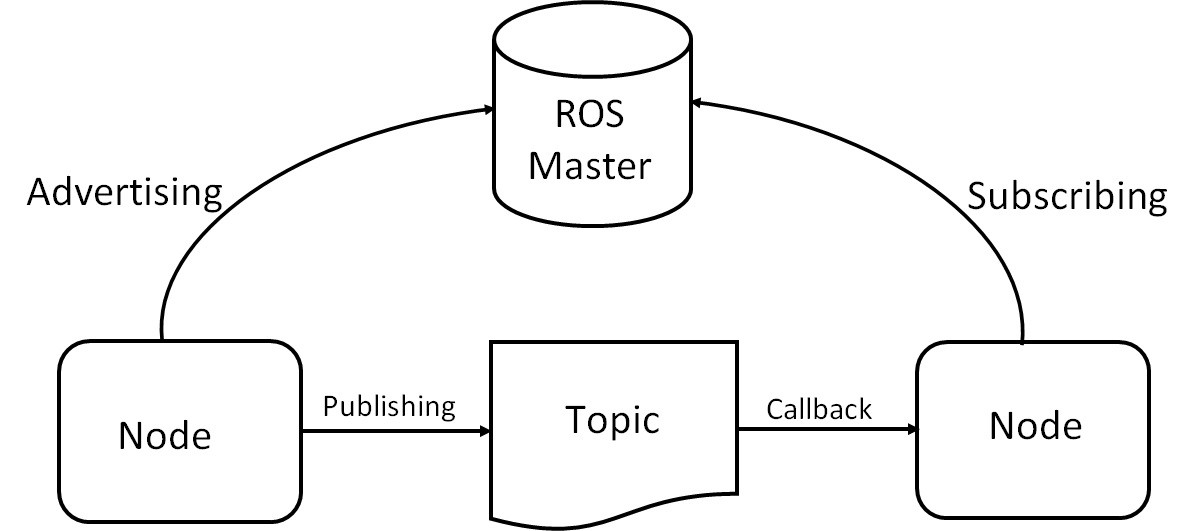
\includegraphics[width=1\textwidth]{/home/tb/Desktop/Master/BA_TB/02_Arbeit_Latex/003_Kapitel2/Bilder/ros_communication}% keine extention: w�hlt jpg f�r DVI
  \caption[Die ROS-Kommunikationsarchitektur]%
           {\label{fig:Die ROS-Kommunikationsarchitektur}%
           Die ROS-Kommunikationsarchitektur. \cite{roscomm}}
\end{center}
\end{figure}


\subsection{Nodes}
\label{subsec:Nodes}

ROS ist ein verteiltes System bestehend aus Prozessen, sogenannten Nodes welche es erm�glichen individuell ausf�hrbare Programme zur Laufzeit einfach miteinander kommunizieren zu lassen. Diese Prozesse sind freilaufend �ber die ROS-Kommunikationsinfrastruktur verbunden.

\subsection{Topics}
\label{subsec:Topics}
Sind Datenbusse �ber welche ROS-Nachrichten asynchron ausgetauscht werden k�nnen. Nodes k�nnen Daten auf verschiedene Topics senden (publish), w�hrend andere Nodes diese Topics auslesen (subscribe) k�nnen, um die Daten weiterzuverarbeiten. Dadurch l�sst sich die Produktion und der Konsum von Informationen entkoppeln. Mit einer solchen Softwarearchitektur k�nnen unabh�ngig entwickelte Softwarekomponenten verwendet und in bestehende Systeme integriert werden. Ein weiterer Vorteil ist dabei das durch Topics klare Schnittstellen zu anderen Nodes festgelegt werden und ein sauberes Programmieren erzwungen wird.

\subsection{Messages}
\label{subsec:Messages}
Um den Datenaustausch �ber Topics zu vereinfachen, nutzt ROS die Standardisierung von Daten und deren Format. Dies wird mit sogenannten ROS-Messages umgesetzt. Diese Messages beschreiben die Datenstrukturen, welche auf ROS-Topics gesendet werden und erm�glicht es ROS-Tools automatisch Quellcode f�r den Message-Typ in verschiedenen Programmiersprachen zu generieren. Als Beispiel kann die ROS-Message sensor{\tiny\_}msgs/Image genannt werden, welche die Breite und H�he wie auch die Pixelcodierung eines auf eine Topic gesendeten Kamera-Frames defniert.

\subsection{Packages}
\label{subsec:Packages}
In ROS wird Software in Packages verarbeitet. Ein Package kann eine ROS-Node enthalten, eine von ROS unabh�ngige Programmbibliothek, ein Datenset von Konfgurations-Dateien, die Software eines Drittanbieters, kurz gesagt jede m�gliche Art von n�tzlichen Software-Modulen. Dabei ist das Ziel dieser Packages ein einfaches Wiederverwenden von Softwarefunktionalit�ten zu erm�glichen.

\section{Einf�hrung in das Catkin Build-System}
\label{sec:Einf�hrung in das Catkin Build-System}
Catkin ist das Meta-Buildsystem von ROS. Es erm�glicht automatische Builds der Software im ROS-Workspace. Unter Ausnutzung des Cross-Platform-Build-Management-Tools CMake werden separat abh�ngige CMake-Projekte in einem Build zu einem gro�en CMake-Projekt zusammengef�hrt.
Dies wird durch eine spezielle Top-Level CMakeLists.txt erreicht. Bevor es CMake gab, musste f�r jede Plattform und f�r jeden Compiler und Linker manuell ein eigenes Makefile geschrieben werden. CMake automatisiert diesen Prozess mittels plattformunabh�ngiger Bauanweisungen f�r Makefiles. CMake generiert Dateien f�r verschiedene Build-Tools wie Make, Ninja, Apple's Xcode und Microsoft Visual Studio. CMake wird auch von einigen IDEs wie Qt-Creator direkt verwendet. Der Build-Prozess mit CMake erfolgt in zwei Schritten. Zun�chst werden Standardbuilddateien aus Konfigurationsdateien (CMakeLists.txt) erstellt. Dann werden die nativen Build-Tools der Plattform f�r das eigentliche Builden verwendet. Unter Linux ist Make das native Build-Tool und das Makefile die Standardbuilddatei. Das Makefile weist Make an wie es ein Programm f�r die verwendete Hardware-Plattform zu kompilieren und zu Linken hat. Jeder Kompilier-Vorgang erzeugt eine Objektdatei, die einer Quelldatei entspricht. Wenn eine Quelldatei erneut kompiliert wurde, m�ssen alle Objektdateien, unabh�ngig davon, ob sie neu erstellt oder aus fr�heren Kompilierungen gespeichert wurden, durch den Linker miteinander verkn�pft werden, um das neue ausf�hrbare Programm zu erstellen. Im Folgenden soll veranschaulicht werden wie der Aufbau einer CMakeLists.txt in ROS gestaltet sein muss, um ausf�hrbaren Programm-Code erzeugen zu k�nnen.




\begin{enumerate}

\item[] \textbf{CMAKE\_MINIMUM\_REQUIRED()} \hfill \\
Legt die minimal erforderliche Version von CMake f�r ein Projekt fest.
Wenn die aktuelle Version von CMake niedriger ist als die erforderliche Version, wird das Projekt nicht mehr verarbeitet und ein Fehler gemeldet.


\item[] \textbf{PROJECT()}\hfill \\
Legt den Namen des Projekts fest und speichert ihn in der Variablen PROJECT\_NAME. Beim Aufruf aus der obersten Ebene (Top-Level) speichert CMakeLists.txt auch den Projektnamen in der Variablen CMAKE\_PROJECT\_NAME.


\item[] \textbf{ADD\_COMPILE\_OPTIONS()}\hfill \\
F�gt Kompilieroptionen unter der Variablen COMPILE\_OPTIONS hinzu. Diese Optionen werden beim kompilieren von Targets aus dem aktuellen Verzeichnis und darunter verwendet. Hier kann zum Beispiel der C++-Standard festgelegt werden.

\item[] \textbf{find\_package()}\hfill \\
Sucht und l�dt Einstellungen aus externen Projekten. <package>\_FOUND wird gesetzt, um anzuzeigen, ob das Paket gefunden wurde. Wenn das Paket gefunden wird, werden paketspezifische Informationen �ber Variablen und importierte Targets bereitgestellt.
Die Funktion wird ben�tigt, um Catkin-Makros zu laden und Abh�ngigkeiten zu anderen ROS-Paketen anzugeben.
Es definiert Abh�ngigkeiten f�r dieses Package.


\item[] \textbf{catkin\_package()}\hfill \\
Dies ist ein Catkin-Makro. Es ist f�r die ROS-spezifische Konfiguration des Pakets verantwortlich. Es ist der wesentliche Teil, der ein ROS-Paket von einem normalen CMake-Projekt unterscheidet. Es deklariert Abh�ngigkeiten f�r Packages welche dieses Package inkludieren wollen.


\item[] \textbf{include\_directiories()}\hfill \\
F�gt die angegebenen Verzeichnisse zu den Verzeichnissen hinzu, in denen der Compiler nach Include-Dateien sucht. Relative Pfade werden als relativ zum aktuellen Quellverzeichnis interpretiert. Die Include-Verzeichnisse werden f�r die aktuelle CMakeLists.txt-Datei der Variablen INCLUDE\_DIRECTORIES hinzugef�gt.


\item[] \textbf{add\_exetutable()}\hfill \\
F�gt dem Projekt eine ausf�hrbare Datei mit den angegebenen Quelldateien hinzu.


\item[] \textbf{target\_link\_libraries()}\hfill \\
Verkn�pft ein Target mit den angegeben Libraries (Linken) auch spezielle Flags k�nnen gesetzt werden.


\end{enumerate}



     % 
%
%% Kapitel: Stand der Technik
%%======================================================================

\chapter{Auswahl der Entwicklungsumgebung}
\label{cha:Auswahl der Entwicklungsumgebung} \index{Auswahl der Entwicklungsumgebung}

Um Software effizient entwickeln zu k{\"o}nnen ist eine geeignete Programmierumgebung unabdingbar. 
Da nicht jede Entwicklungsumgebung mit ROS kompatibel ist und jeder dieser IDEs ihre vor und Nachteile besitzt wurde wurden Methoden der Entscheidungstheorie angewandt um die bestm{\"o}gliche IDE auszuw{\"a}hlen.

Durch die Methode Paarweiser Vergleich wurden die Gewichtungen vor eine Nutzweranalyse ermittelt. Es stellte sich heraus das bei der Auswahl einer IDE vorallem wichtig ist das Sie mit dem Betriebssystemlinux kompatibel ist, sie den Code mit CMake buildet und einen guten Debug-Modus hat.






\begin{figure}[H]
\begin{center}
  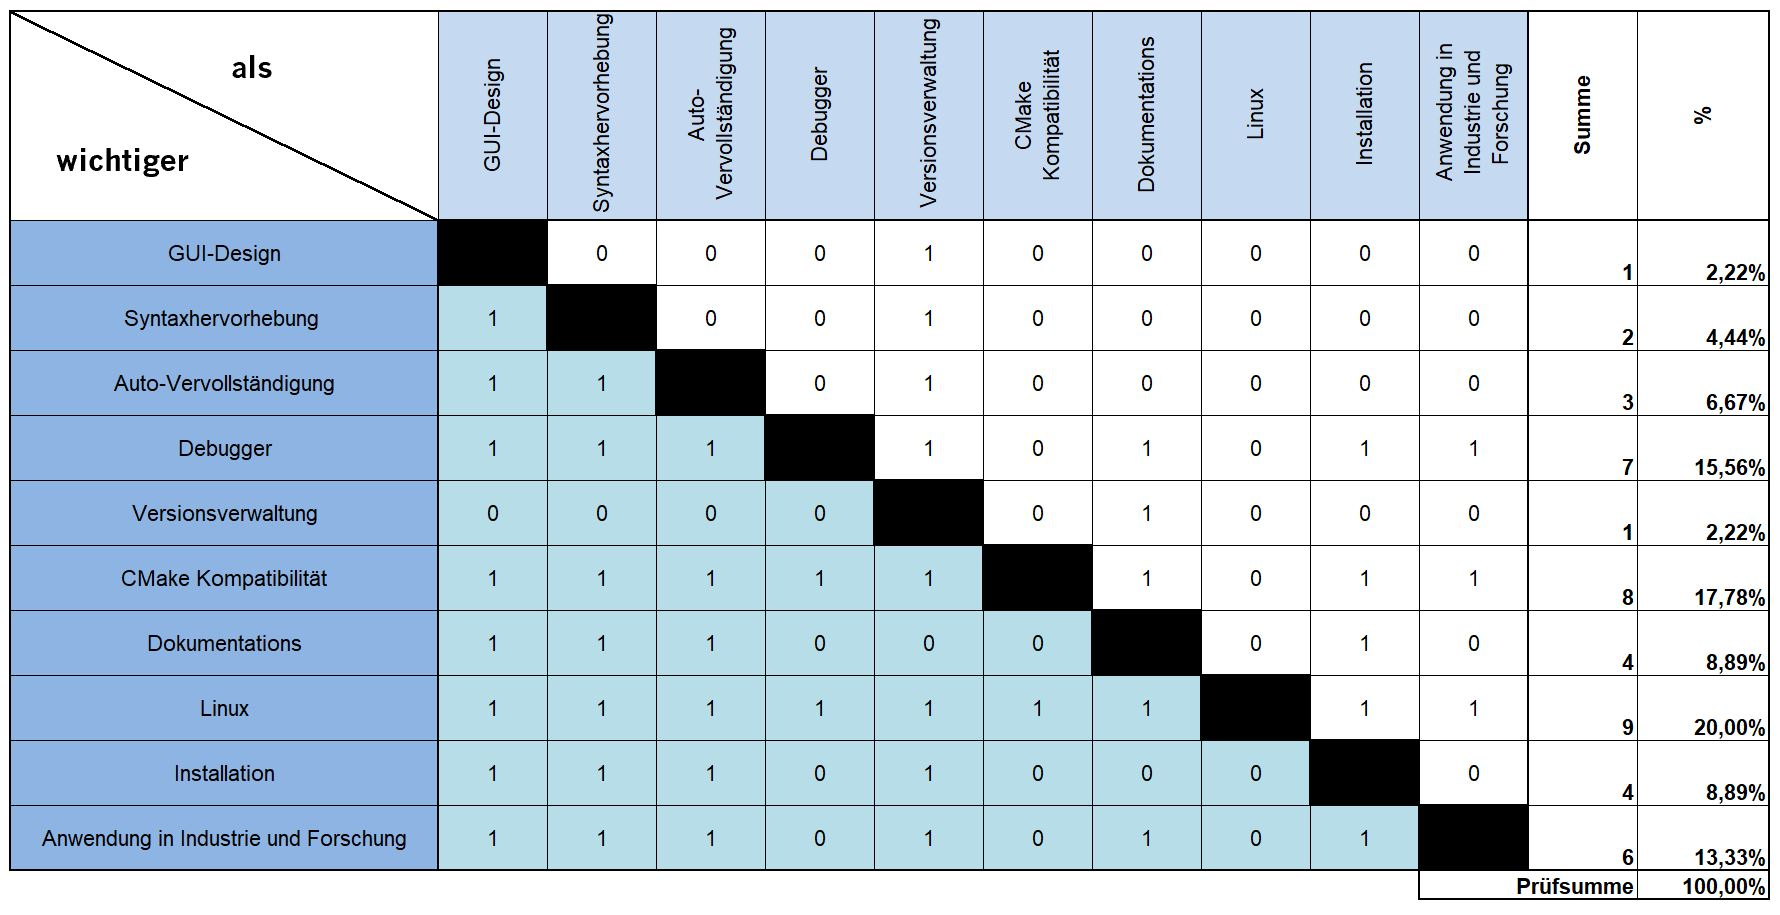
\includegraphics[width=1\textwidth]{/home/tb/Desktop/Master/BA_TB/02_Arbeit_Latex/004_Kapitel3/Bilder/paarweiser_vergleich_ide}% keine extention: wählt jpg für DVI
  \caption[PaarweiserVergleichIDE]%
           {\label{fig:PaarweiserVergleichIDE}%
           Paarweiser Vergleich wichtiger Attribute einer Entwicklungsumgebung.}
\end{center}
\end{figure}

Durch die Nutzwertanalyse konnten nun die zur Verfügung stehenden Entwicklungsumgebungen verglichen werden. 

\begin{figure}[H]
\begin{center}
  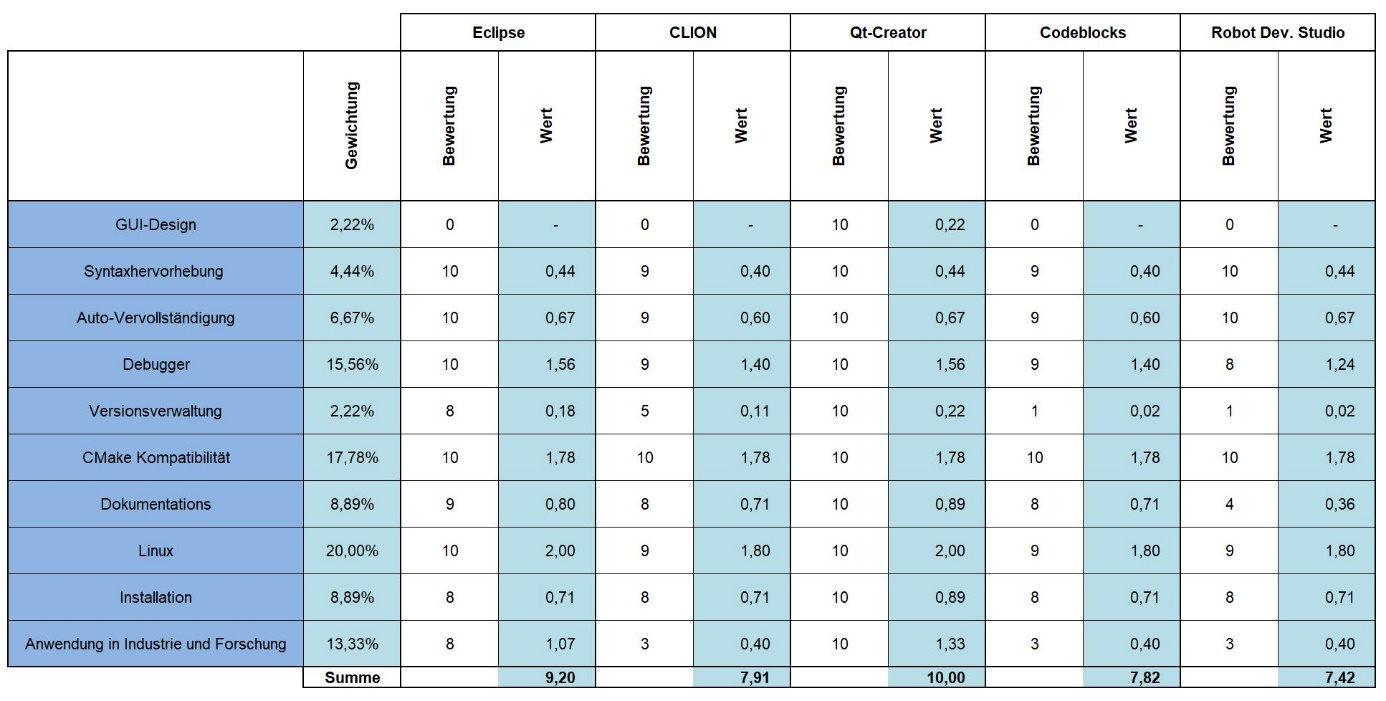
\includegraphics[width=1\textwidth]{/home/tb/Desktop/Master/BA_TB/02_Arbeit_Latex/004_Kapitel3/Bilder/nutzwertanalyse_ide}% keine extention: wählt jpg für DVI
  \caption[NutzwertAnalyseIDE]%
           {\label{fig:NutzwertAnalyseIDE}%
           Auswertung der Nutzwertanalyse von verschiedenen Entwicklungsumgebungen.}
\end{center}
\end{figure}


Wie in Abbildung [X] zu sehen ist, ergibt sich durch die Auswertung der Nutzwertanalyse das die Qt-Creator DIE die beste Wahl f{\"u}r die gestellten Anforderungen ist. Vorallem weil sie stark in der Industrie und Forschung angewandt wird viel die Wahl auf den Qt-Creator. Zudem ist Qt mit zugeh{\"o}rigem ROS-Plugin sehr einfach mit einem run skript zu installieren.
%https://ros-qtc-plugin.readthedocs.io/en/latest/_source/How-to-Install-Users.html



%\begin{enumerate}

%\item
%\end{enumerate}



%
%% Kapitel: Kapitel 4
%%======================================================================

\chapter{Auswahl der Simulationsumgebung}
\label{cha:Auswahl der Simulationsumgebung } \index{Einf{\"u}hrung in die Objekterkennung in Bildern}
%
%


Das Testen von Software f{\"u}r autonome Fahrzeuge in einer Simulationsumgebung (Software in the Loop) ist heute bereits zum Standard in der Automobilindustrie geworden.
Fahrsimulatoren stellen ein wichtiges Forschungs- und industrielles Entwicklungswerkzeug dar. Im Bereich der sicherheitsrelevanten Fahrerassistenzsysteme beginnt die Funktionsentwicklung verst{\"a}rkt mit Softwaremodellen. Software kann zu einem fr{\"u}hen Zeitpunkt in Fahrsimulatoren analysiert und Zusammenh{\"a}nge mit anderen Funktionen teilweise kosteng{\"u}nstiger als mit realen Prototypen untersucht werden. Die f{\"u}r einzelne Fragestellungen erforderlichen Fahrsituationen werden in einer Simulation gut kontrolliert und reproduzierbar dargestellt. Dabei besteht bei einer Simulation keine Gefahr f{\"u}r das reelle Fahrzeug. So lassen sich Pr{\"u}f- und Diagnose Software effizient auswerten. F{\"u}r das autonome Modellfahrzeug der Hochschule Karlsruhe soll deshalb eine geeignete Simulationsumgebung gefunden werden in der Bildverarbeitungs-Algorithmen und gesamte Softwarearchitekturen auf ihr Verhalten getestet werden k{\"o}nnen. Um die beste Wahl f{\"u}r das CaroloCup Team zu treffen wurde deshalb wieder eine Nutzwertanalyse der m{\"o}glichen Simulationsumgebungen erstellt. 
%[https://cuvillier.de/uploads/preview/public_file/2747/9783867277273.pdf]



\begin{figure}[H]
\begin{center}
  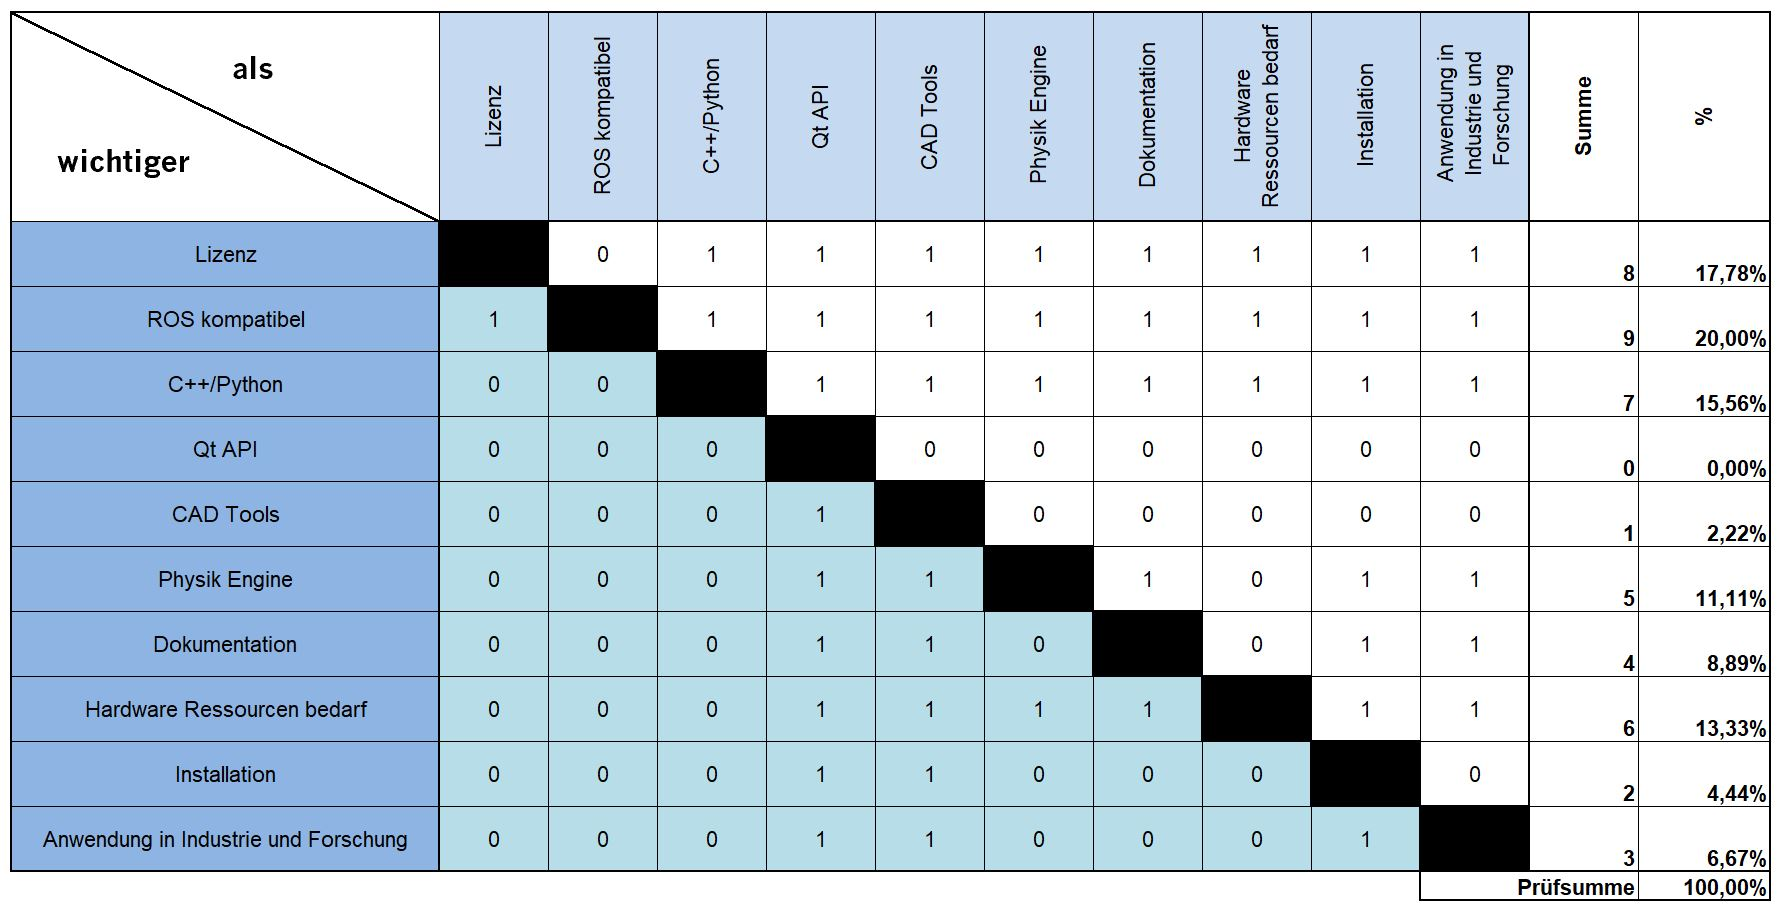
\includegraphics[width=1\textwidth]{/home/tb/Desktop/Master/BA_TB/02_Arbeit_Latex/005_Kapitel4/Bilder/paarweiser_vergleich_sim}% keine extention: w�hlt jpg f�r DVI
  \caption[PaarweiserVergleichSIM]%
           {\label{fig:PaarweiserVergleichSIM}%
           Paarweiser Vergleich wichtiger Attribute einer Simulationsumgebung.}
\end{center}
\end{figure}

Nach Auswertung des Paarweisen Vergleichs zeigt sich, dass vorallem die Kompatibilit{\"a}t zu ROS eine sehr wichtige Rolle bei der Auswahl der Simulaionsumgebung spielt.
Auch sollte die Simulationsumgebung keine kostenpflichtige Lizenz ben{\"o}tigen, da die Kosten nach CaroloCup-Regelwerk so niedrig wie m{\"o}glich gehalten werden sollen. Die Simulationsumgebung sollte auch eine C++- oder Python-API besitzen um das Fahrzeug mit der Bildverarbeitung zu koppeln.


\begin{figure}[H]
\begin{center}
  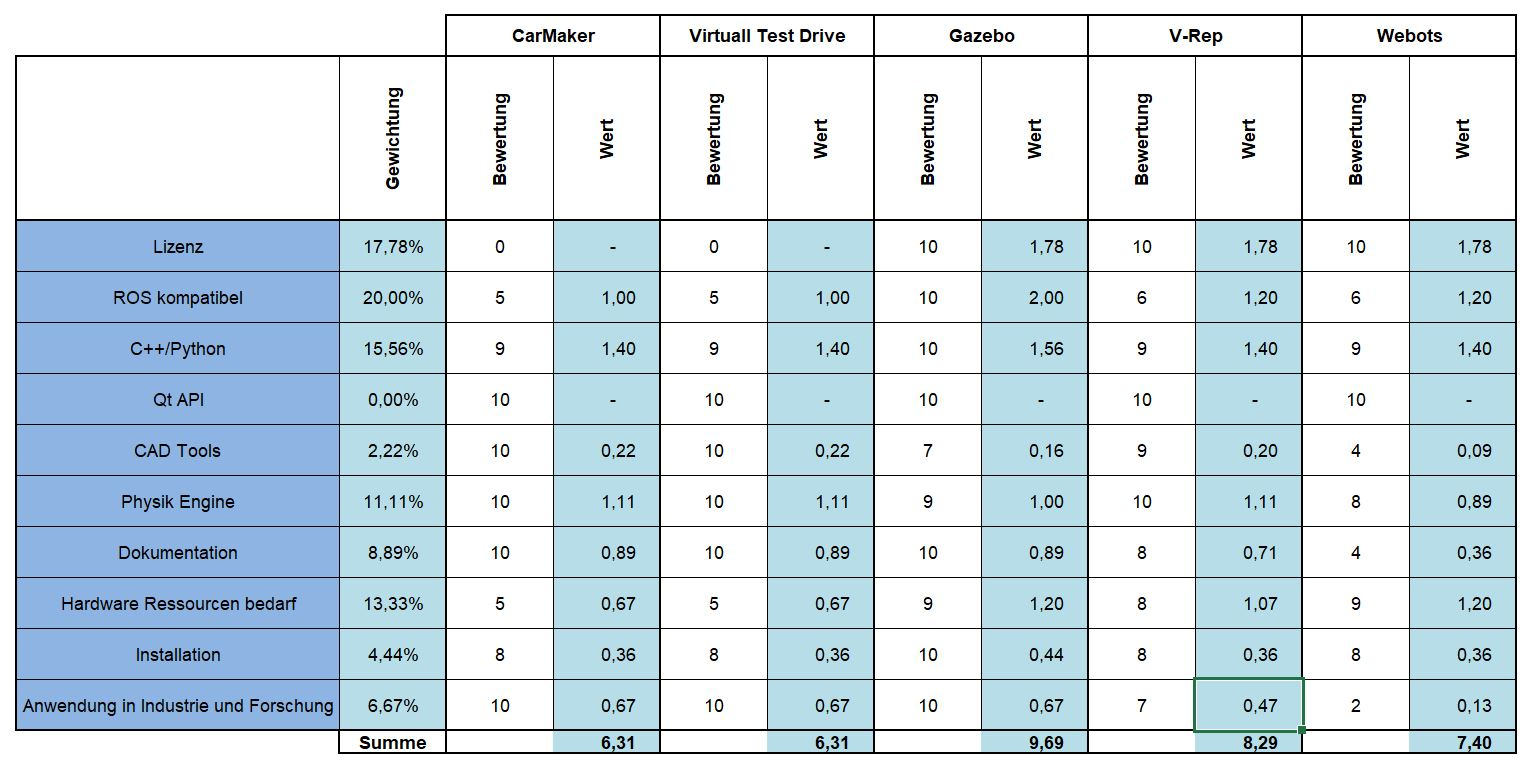
\includegraphics[width=1\textwidth]{/home/tb/Desktop/Master/BA_TB/02_Arbeit_Latex/005_Kapitel4/Bilder/nutzwertanalyse_sim}% keine extention: w�hlt jpg f�r DVI
  \caption[NutzwertAnalyseSIM]%
           {\label{fig:NutzwertAnalyseSIM}%
           Auswertung der Nutzwertanalyse von verschiedenen Simulationsumgebungen.}
\end{center}
\end{figure}

Die zwei Simulationsumgebungen mit der h{\"o}chsten Punktzahl (V-REP und Gazebo) sollen anschlie�end noch einmal n{\"a}her beschrieben werden.




\section{Die Virtual Robot Experimentation Platform Simulationsumgebung}
\label{sec:Die Virtual Robot Experimentation Platform Simulationsumgebung}
Die Virtual Robot Experimentation Platform (V-REP) ist eine dreidimensionale plattform{\"u}bergreifende Simulations-Engine von Coppelia Robotics. Sie unterst{\"u}tzt unter anderem C/C ++, Python, Lua, Octave und Matlab. Zur Simulation der Physik stehen verschiedene Engines zur Verf{\"u}gung, beispielsweise Newton, Bullet, Open Dynamics Engine oder Vortex.
Verf{\"u}gbar ist die Engine f{\"u}r MacOS, Linux und Windows.
V-REP bietet eine gro�e Auswahl an Robotern, einschlie�lich Bi-Pedal-, Hexapod-, Rad-, Flug- und schlangen{\"a}hnlichen Robotern. Zudem sind auch Aktoren und Sensoren, welche durch Plugins integriert werden k{\"o}nnen, verf{\"u}gbar.
Es gibt verschiedene Optionen f{\"u}r die Programmierung von Funktionen, wie etwa Skripte die Roboter ansteuern, Plug-Ins und auch ROS-Knoten, die alle {\"u}ber die Remote-API eine Verbindung zu V-REP herstellen k{\"o}nnen
Vor allem bei der Konstruktion von neuen Robotern und Welten kann V-REP punkten.
Mit CAD designte Modelle k{\"o}nnen von Robotern in Echtzeit manipuliert werden.
Das Interagieren (z.B. verschieben oder hinzuf{\"u}gen) von Objekten wird erm{\"o}glicht. 
Es ist m{\"o}glich, Meshes zu vereinfachen, zu teilen und zu kombinieren.Meshes sind eine vereinfachte Oberfl{\"a}chenbeschreibungen aus dreidimensionalen Bilddateien. Dies erm{\"o}glicht es, die Dreieckszahl importierter Modelle zu optimieren und Meshes mit Roboteraktuatoren zu manipulieren. 


\section{Die Gazebo Simulationsumgebung}
\label{sec:Die Gazebo Simulationsumgebung}
Ist ein Open Source 3D-Simulator der f{\"u}r die Simulation von Robotern in verschiedenen, komplexen Szenarien erstellt wurde.
Begonnen hat die Entwicklung von Gazebo im Herbst 2002. Im Jahr 2009 wurde das Robot Operating System (ROS) in das Gazebo-Projekt integriert und ist seitdem eines der meistgenutzten Tools in der ROS Community. 2012 wurde die Verwaltung des Open-Source-Projekts Gazebo von der Open Source Robotics Foundation (OSRF) {\"u}bernommen und wird seitdem von OSRF und einer aktiven Community weiterentwickelt. 
Die Physik-Engines Open Dynamics Engine, Bullet, Simbody oder das Dynamic Animation and Robotics Toolkit k{\"o}nnen in Gazebo verwendet werden um die physikalischen Gegenheiten der Simulationsumgebung zu berechnen. Die Open Dynamics Engine ist in der Standardkonfiguration die aktive Physik-Engine.
Durch C++- oder Python-Plugins ist es auch m{\"o}glich Objekte oder die Physik zur Laufzeit der Simulations anzusteuern.
Verschiedene Sensor-Plugins sind in der Gazebo-ROS-API bereits integriert wie etwa Kamera-Sensoren oder eine Ackermann-Lenkung f{\"u}r Fahrzeuge.
Neben diesen Punkten bietet der Gazebo-Simulator viele Anwendungsbeispiele, von einfachen Einstiegsmodellen bis hin zu komplexen Modellen wie Roboterforschungsplattformen mit vielen verschiedenen Sensoren. Dies erm{\"o}glicht auch Entwicklern, die das Framework noch nicht kennen, einen schnellen Einstieg.
Gazebo nutzt unterschiedliche Software-Bibliotheken f{\"u}r die physikalische Simulation, das Rendering oder der Erzeugung von Sensordaten. Gazebo realisiert die Simulation {\"u}ber ein Client-Server Model.
Der gzserver ist f{\"u}r die Simulation der Physik das Rendering und dem Berechnen von Sensordaten zust{\"a}ndig. Der gzclient visualisiert die Simulation f{\"u}r den Benutzer. Durch diese Abstraktion ist es m{\"o}glich Gazebo headless (ohne grafische Ausgabe) laufen zu lassen. Dadurch wird die Simulation nicht visualisiert. Dies f{\"u}hrt zu einem niedrigeren Bedarf an Rechenressourcen.
Im Gegensatz zu V-REP bietet Gazebo weniger M{\"o}glichkeiten um Roboter in der Simulationsumgebung zu modellieren.
Die Modellierung in Gazebo kann {\"u}ber das SDF (Simulation Description Format), einem XML Format zur Beschreibung
von Objekten und Umgebungen speziell f{\"u}r den Einsatz in der Robotersimulation, bewerkstelligt werden was f{\"u}r die Simulation f{\"u}r die Anforderungen des Wettbewerbsteams der Hochschule Karlsruhe ausreichen ist.


%http://lenkaspace.net/tutorials/programming/robotSimulatorsComparison
%https://autonomesysteme.informatik.haw-hamburg.de/papers/2018Dannenberg.pdf


\section{Begr{\"u}ndung der Auswahl}
\label{sec:Begr{\"u}ndung der Auswahl}
Nach abwiegen aller Vor- und Nachteile der beiden Simulationumgebungen wurde sich f{\"u}r den Gazebo-Simulator entschieden. Die Hauptgr{\"u}nde daf{\"u}r waren, dass Gazebo schon bereits nativ mit ROS installiert wird. ROS-Gazebo-Plugins werden von den Entwicklern der Open Source Robotics Foundation betreut und sind daher wengier fehlerbehaftet. Gazebo stellt auch weniger Anforderungen an die Hardware Ressourcen im Gegensatz zu V-REP, dadurch k{\"o}nnte jedes neue Mitglied des Mechatronik Competition Teams Gazebo auf seinem eigenen Ger{\"a}t installieren. [Link hardware]
Die Kommunikation zwischen V-REP und ROS ist auch nicht von der selben Qualit{\"a}t wie der von ROS-Gazebo. Es ist nicht m{\"o}glich V-REP {\"u}ber Roslaunch-Dateien  aufzurufen. Zudem werden {\"u}ber die V-REP-ROS-API ROS-Nachrichten {\"u}ber ein LUA-Skript geparst was zu Performanznachteilen gegen{\"u}ber Gazebo f{\"u}hrt.



\section{Das SDF Format - System Description File}
\label{sec:Das SDF Format - System Description File}
SDF ist ein XML-Format, das Objekte und Umgebungen f�r Robotersimulatoren, Visualisierung und Steuerung beschreibt. Urspr{\"u}nglich als Teil des Gazebo-Robotersimulators entwickelt, wurde SDF unter Ber{\"u}cksichtigung wissenschaftlicher Roboteranwendungen entwickelt. Im Laufe der Jahre hat sich SDF zu einem stabilen, robusten und erweiterbaren Format entwickelt, das alle Aspekte von Robotern, statischen und dynamischen Objekten, Beleuchtung, Gel{\"a}nde und sogar Physik beschreiben kann.

\section{Das World File}
\label{sec:Das World File}
Das World File definiert durch SDF die zu simulierende Welt mit all ihren Komponenten. Es k{\"o}nnen Roboter oder Sensoren mit einer Welt verkn{\"u}pft, die Beleuchtung und Physikalischen Eigenschaft definiert, als auch statische Komponenten eingef{\"u}gt werden. Die World-Datei wird von dem gzserver eingelesen welcher nach den Definitionen die Welt generiert.



\section{Das Model File}
\label{sec:Das Model File}
Eine Modell-Datei beschreibt eine einzelne Einheit der Welt im SDF-Format. Dies k{\"o}nnte Beispielweise ein Fahrzeug f{\"u}r den CaroloCup sein. Einzelne Modell-Deteien k{\"o}nnen zusammen in ein World-File integriert werden.
Wie etwa verschiedene Fahrbahnsegmente.
Dies erm{\"o}glicht einen Modularen Aufbau und sorgt f{\"u}r bessere Lesbarkeit.
Die erste Hauptkomponente zum Beschreiben eines Modells ist der Link (<link>). Ein oder mehrere Links Formen ein Modell. Der Link kann viele verschiedene physikalische Attribute besitzen, wie die Masse (<mass>), das Tr{\"a}gheitsmoment(<inertial>) oder Reibwerte(<friction>). Des weiteren besitzt ein Link ein Kollisionsattribut (<collision>) wor{\"u}ber durch Angabe der geometrischen Gr{\"o}�e die Kollision mit anderen Komponenten der Welt errechnet wird. Eine weitere Komponente ist die visuelle Komponente(<visual>) sie kann optional die Geometrie des Links in der Simulation visualisieren. Auch Sensor-Komponenten(<sensor>) k{\"o}nnen in Links integriert werden, wie etwa ein Kamera-Sensor. Die zweite, optionale Hauptkomponente ist ein Gelenk (<joint>). Auch hiervon k{\"o}nnen mehrere in einem Modell existieren. Ein Gelenk verbindet zwei Links in einer Eltern-Kind-Beziehung miteinander. Verschiedene Gelenk-Typen k{\"o}nnen definiert werden wie etwa einem Drehgelenk(<jointtype=?revolute?>) f{\"u}r ein Rad oder ein Kugelgelenk (<jointtype=?ball?>) f{\"u}r eine Kamera. Durch Plugins(<plugin>) etwa geschrieben in C++ oder Python k{\"o}nnen zur Laufzeit verschiedene Funktionalit{\"a}ten f{\"u}r eine Simulation erg{\"a}nzt werden. Die R{\"a}der eines Fahrzeugs k{\"o}nnen dadurch angesteuert oder Kamera-Sensorwerte an eine ROS-Node {\"u}bermittelt werden.



%https://autonomesysteme.informatik.haw-hamburg.de/papers/2018Dannenberg.pdf
%
%% Kapitel: Kapitel 4
%%======================================================================

\chapter{Erzeugung von simulierten Verkehrssitationen}
\label{cha:Erzeugung von simulierten Verkehrssitationen} \index{Erzeugung von simulierten Verkehrssitationen}

Um ein Testen der Bildverarbeitungsalgorithmen zu erm�glichen soll eine Simulationsumgebung implementiert werden. Mit der in \ref{cha:Auswahl der Entwicklungsumgebung}  ausgew�hlten Simulationsumgebung Gazebo wurde daf�r eine Fahrbahn und ein mit einem Controller gesteuertes Fahrzeug mit Kamera implementiert. In diesem Kapitel wird der Aufbau und die Verwendung der Simulationsumgebung n�her beschrieben.


\section{Erstellung der Fahrbahn}
\label{sec:Erstellung der Fahrbahn}

Mit Gazebo ist es m�glich Bilddateien durch OGRE (Object-Oriented Graphics Rendering Engine) in die Simulationsumgebung einzuladen und entsprechend darzustellen. Es bedurfte eines geeigneten Software-Werkzeugs um eine Fahrbahn entsprechend den Regeln des Carolo-Cups zu modellieren.
Vektorbasierte 2D-Grafiken k�nnen zum Beispiel mit Inkscape oder Adobe Illustrator designt werden wie es in \cite{gazebovrepeval} getan wurde. Auch w�re es denkbar die 3D-Grafiksuit Blender oder ein entsprechendes CAD-Programm zu verwenden. Um es dem Anwender zu vereinfachen wurde sich aber f�r eine andere Methode entschieden. Cairo ist eine 2D-Grafikbibliothek. Sie erm�glicht es vektorbasierte Grafiken zu erzeugen. Mit der Python-API von Cairo namens Pycairo wurde die Erzeugung von Fahrbahnsegmenten automatisiert. Die Idee war es einen Modularen Aufbau von Fahrbahnsegmenten zu realisieren, welche durch Pycario erzeugt und automatisiert in das Gazebo-Modell-Format konvertiert und �ber das Gazebo-Client-Interface zusammengef�gt werden k�nnen. Dazu wurden f�r jedes Modell der Fahrbahn Python-Skripte geschrieben, welche Bilddateien im PNG-Format f�r jede Fahrsituation erzeugen. Im Folgenden werden diese einzelnen Python-Skripte n�her beschrieben.


\begin{enumerate}

\item[] \textbf{Gerade Strecken} \hfill \\
Als Eingabeparameter nimmt das Skript die L�nge der Fahrbahn und den Offset f�r den Start der Mittellinienrasterung entgegen. Anschlie�end speichert es das Segment in einer PNG-Datei. Die Breite der Fahrspuren betr�gt in der Simulation 400mm. Die Mittel- und Au�enlinien besitzen eine Breite von 20mm. Die l�nge einer Mittellinie ist mit 200mm bemessen, genau wie auch deren Abstand untereinander.

\begin{figure}[H]
\begin{center}
  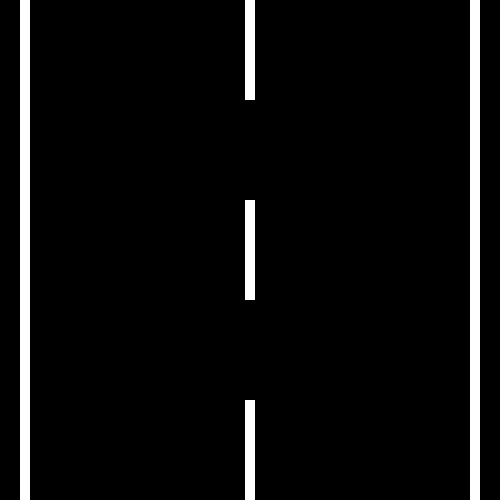
\includegraphics[width=0.3\textwidth]{/home/tb/Desktop/Master/BA_TB/02_Arbeit_Latex/006_Kapitel5/Bilder/straight_1m}% keine extention: w�hlt jpg f�r DVI
  \caption[Gerades Streckensegment]%
           {\label{fig:GeradeSrecke}%
           Gerades Streckensegment}
\end{center}
\end{figure}



\item[] \textbf{Kurven}\hfill \\
Als Eingangsparameter nimmt das Skript den Radius der Kurve entgegen, wie auch den Offset der Mittellinienrasterung. Anschlie�end speichert es das Segment in einer PNG-Datei.
Die Kurvensegmente besitzen die selbe Dimensionierung wie die geraden Streckenabschnitte.

\begin{figure}[H]
\begin{center}
  
\includegraphics[width=0.3\textwidth]{/home/tb/Desktop/Master/BA_TB/02_Arbeit_Latex/006_Kapitel5/Bilder/Kurve}% keine extention: w�hlt jpg f�r DVI
  \caption[Kurvensegment]%
           {\label{fig:Kurve}%
           Kurvensegment}
\end{center}
\end{figure}



\item[] \textbf{Ziellinie}\hfill \\
Dieses Skript erzeugt die Startlinie ohne Eingabeparameter.
Die Startlinie besteht aus einem karierten Muster welches aus Quadraten mit 50mm Seitenl�nge aufgebaut ist.

\begin{figure}[H]
\begin{center}
  
\includegraphics[width=0.5\textwidth]{/home/tb/Desktop/Master/BA_TB/02_Arbeit_Latex/006_Kapitel5/Bilder/ziel}% keine extention: w�hlt jpg f�r DVI
  \caption[Zielliniensegment]%
           {\label{fig:Zielliniensegment}%
           Zielliniensegment}
\end{center}
\end{figure}

\item[] \textbf{Geschwindigkeitsbegrenzungen}\hfill \\
Als Eingangsparameter nimmt das Skript den Wert der Geschwindigkeitsbegrenzung entgegen. Anschlie�end speichert es das Segment in einer PNG-Datei. Auf der Fahrbahn besitzen die Markierungen eine H�he von 400mm und eine Breite von 150mm.

\begin{figure}[H]
\begin{center}
  
\includegraphics[width=0.5\textwidth]{/home/tb/Desktop/Master/BA_TB/02_Arbeit_Latex/006_Kapitel5/Bilder/roadspeedsigngs}% keine extention: w�hlt jpg f�r DVI
  \caption[Geschwindigkeitsbegrenzungssegmente]%
           {\label{fig:Geschwindigkeitsbegrenzungssegmente}%
           Geschwindigkeitsbegrenzungssegmente}
\end{center}
\end{figure}


\item[] \textbf{Zebrastreifen}\hfill \\
Das Skript erzeugt einen Zebrastreifen ohne Eingabeparameter.
Die einzelnen Streifen besitzen eine Breite von 40mm und eine H�he von 400mm. 

\begin{figure}[H]
\begin{center}
  
\includegraphics[width=0.3\textwidth]{/home/tb/Desktop/Master/BA_TB/02_Arbeit_Latex/006_Kapitel5/Bilder/crosswalk}% keine extention: w�hlt jpg f�r DVI
  \caption[Zebrastreifensegment]%
           {\label{fig:Zebrastreifensegment}%
           Zebrastreifensegment}
\end{center}
\end{figure}

\item[] \textbf{Kreuzungen}\hfill \\
Die verschiedenen Arten m�glicher Kreuzungen wurden aus einzelnen durch Pycairo erzeugten Modulen in Inkscape zu einer Einheit zusammengef�hrt.

\begin{figure}[H]
\begin{center}
  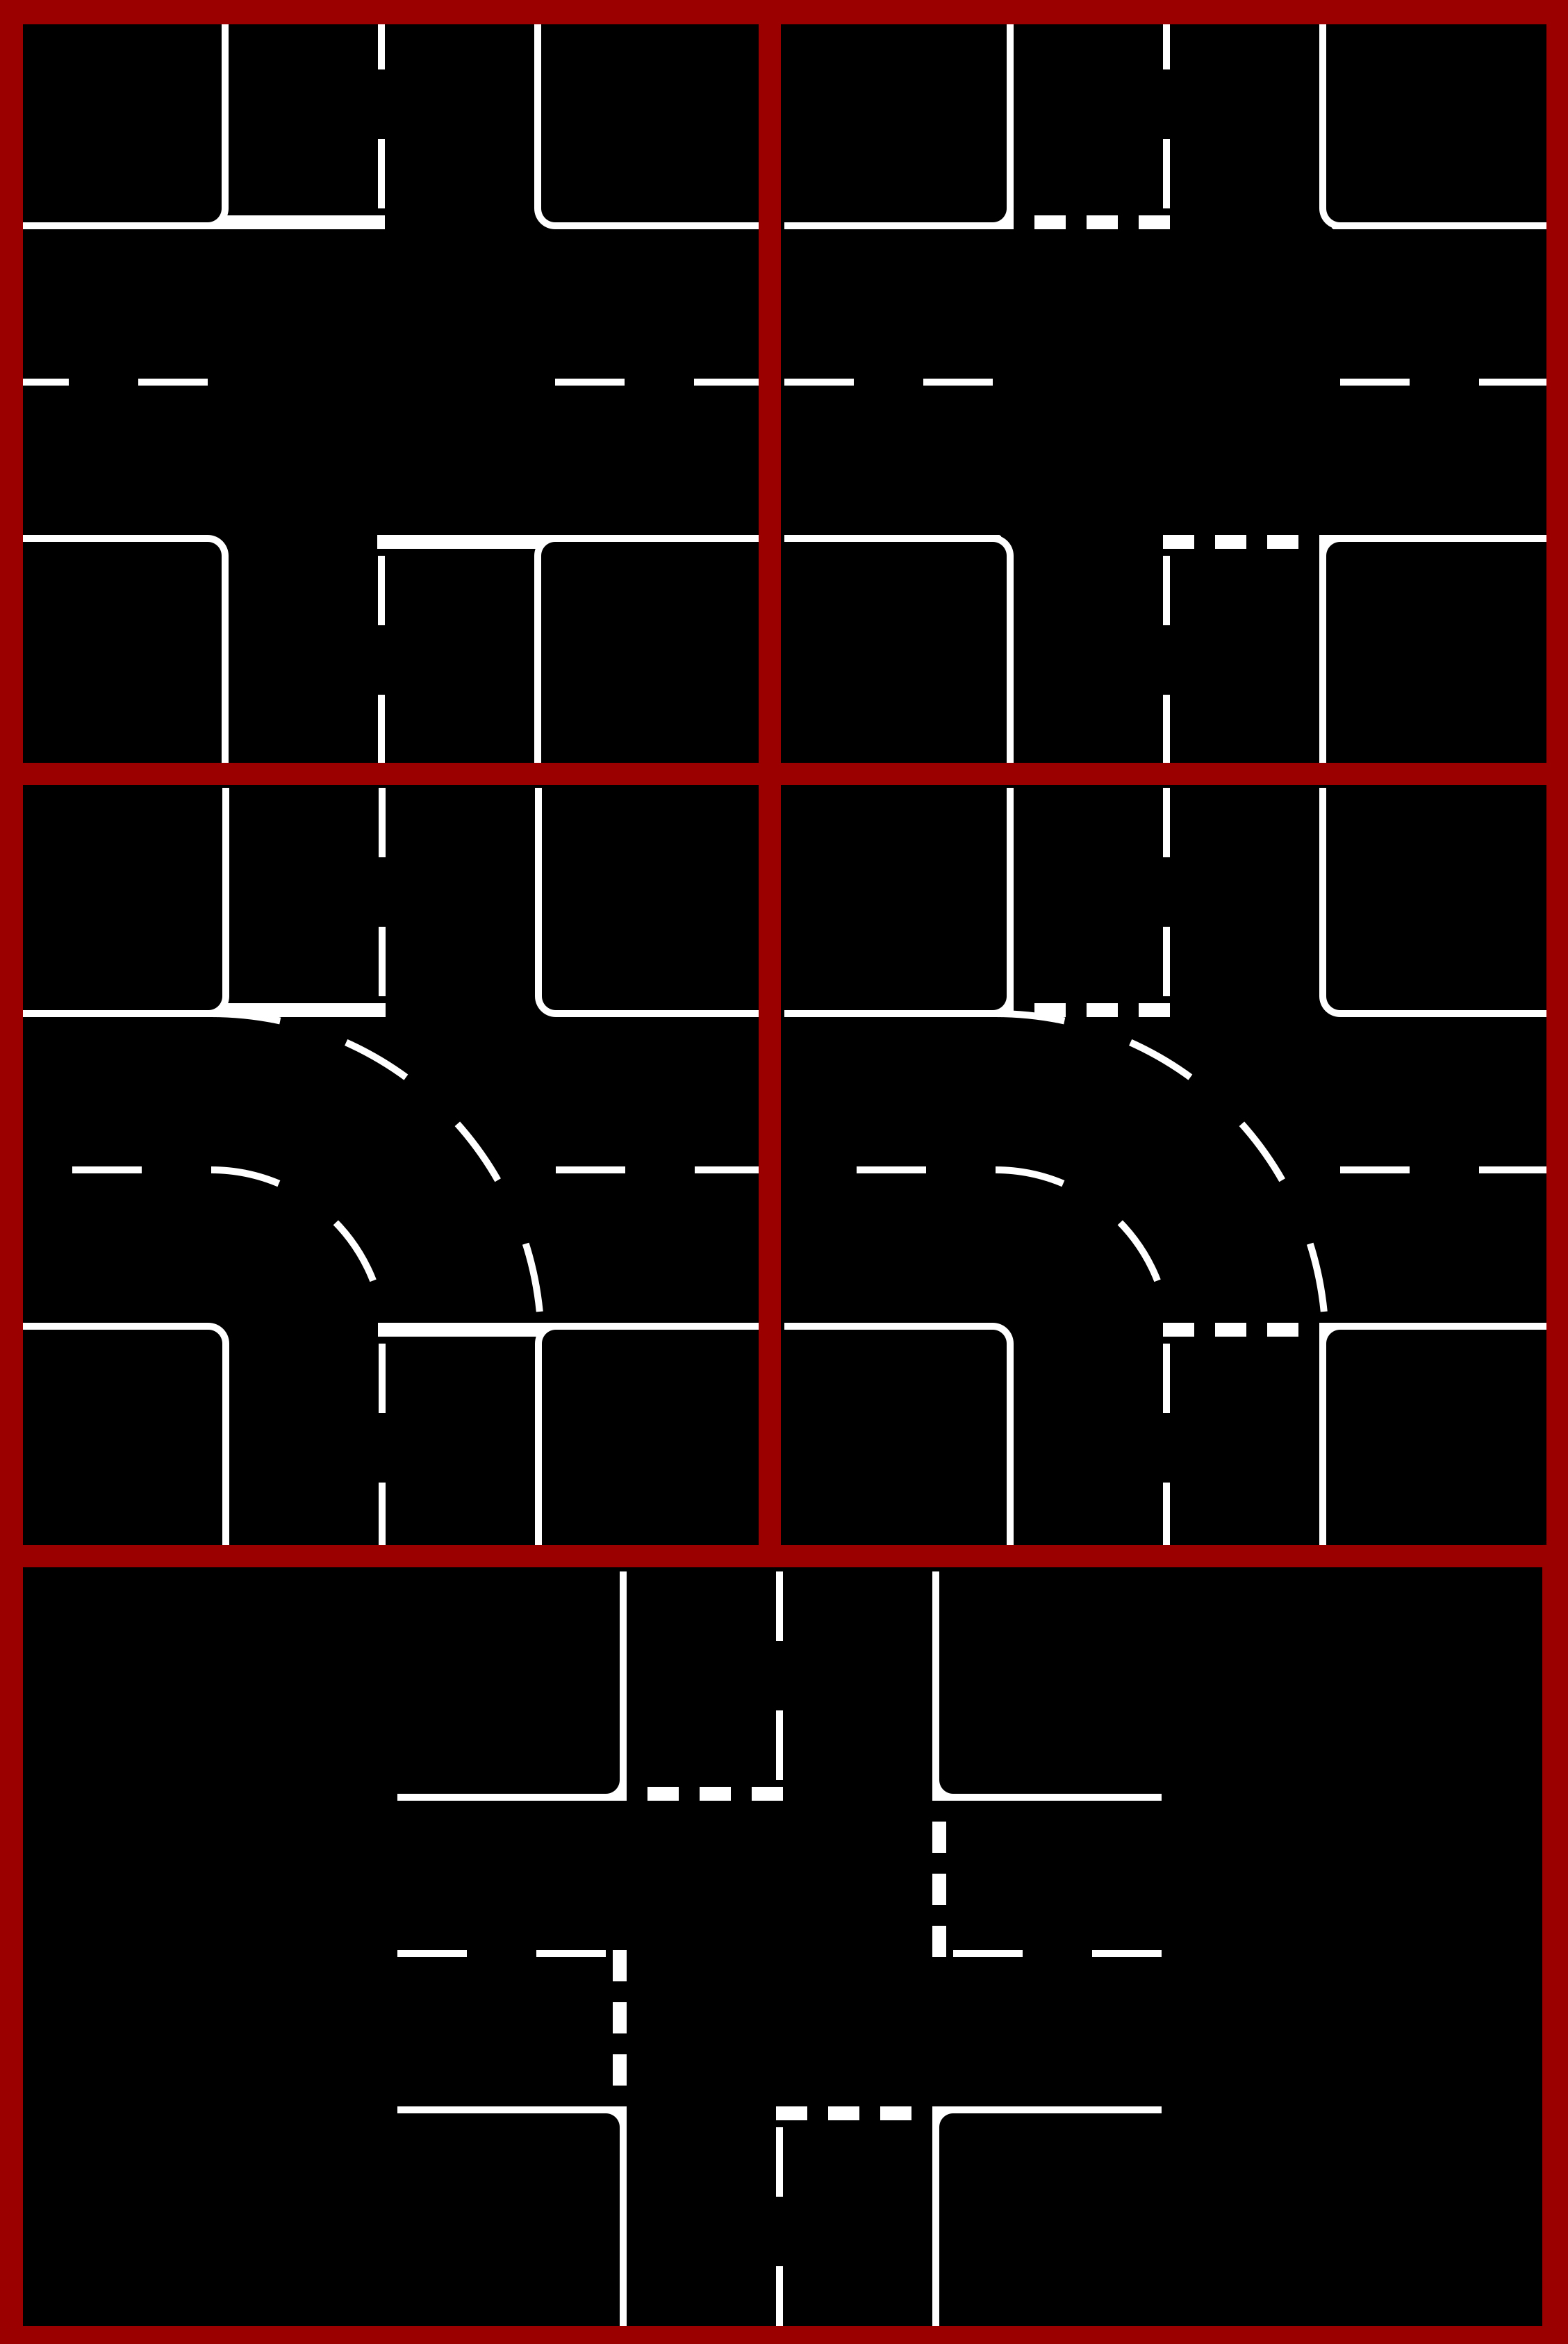
\includegraphics[width=0.3\textwidth]{/home/tb/Desktop/Master/BA_TB/02_Arbeit_Latex/006_Kapitel5/Bilder/crossings}% keine extention: w�hlt jpg f�r DVI
  \caption[Kreuzungssegmente]%
           {\label{fig:Kreuzungssegmente}%
           Kreuzungssegmente}
\end{center}
\end{figure}


\item[] \textbf{Startbox und Parkbereich}\hfill \\
Der Parkbereich wurde zusammen mit der Startbox aus einzelnen Pycairo-Modulen in Inkscape zusammengef�hrt. Da diese Segmente immer gleich aufgebaut sind, werden keine Eingabeparameter ben�tigt. 

\begin{figure}[H]
\begin{center}
  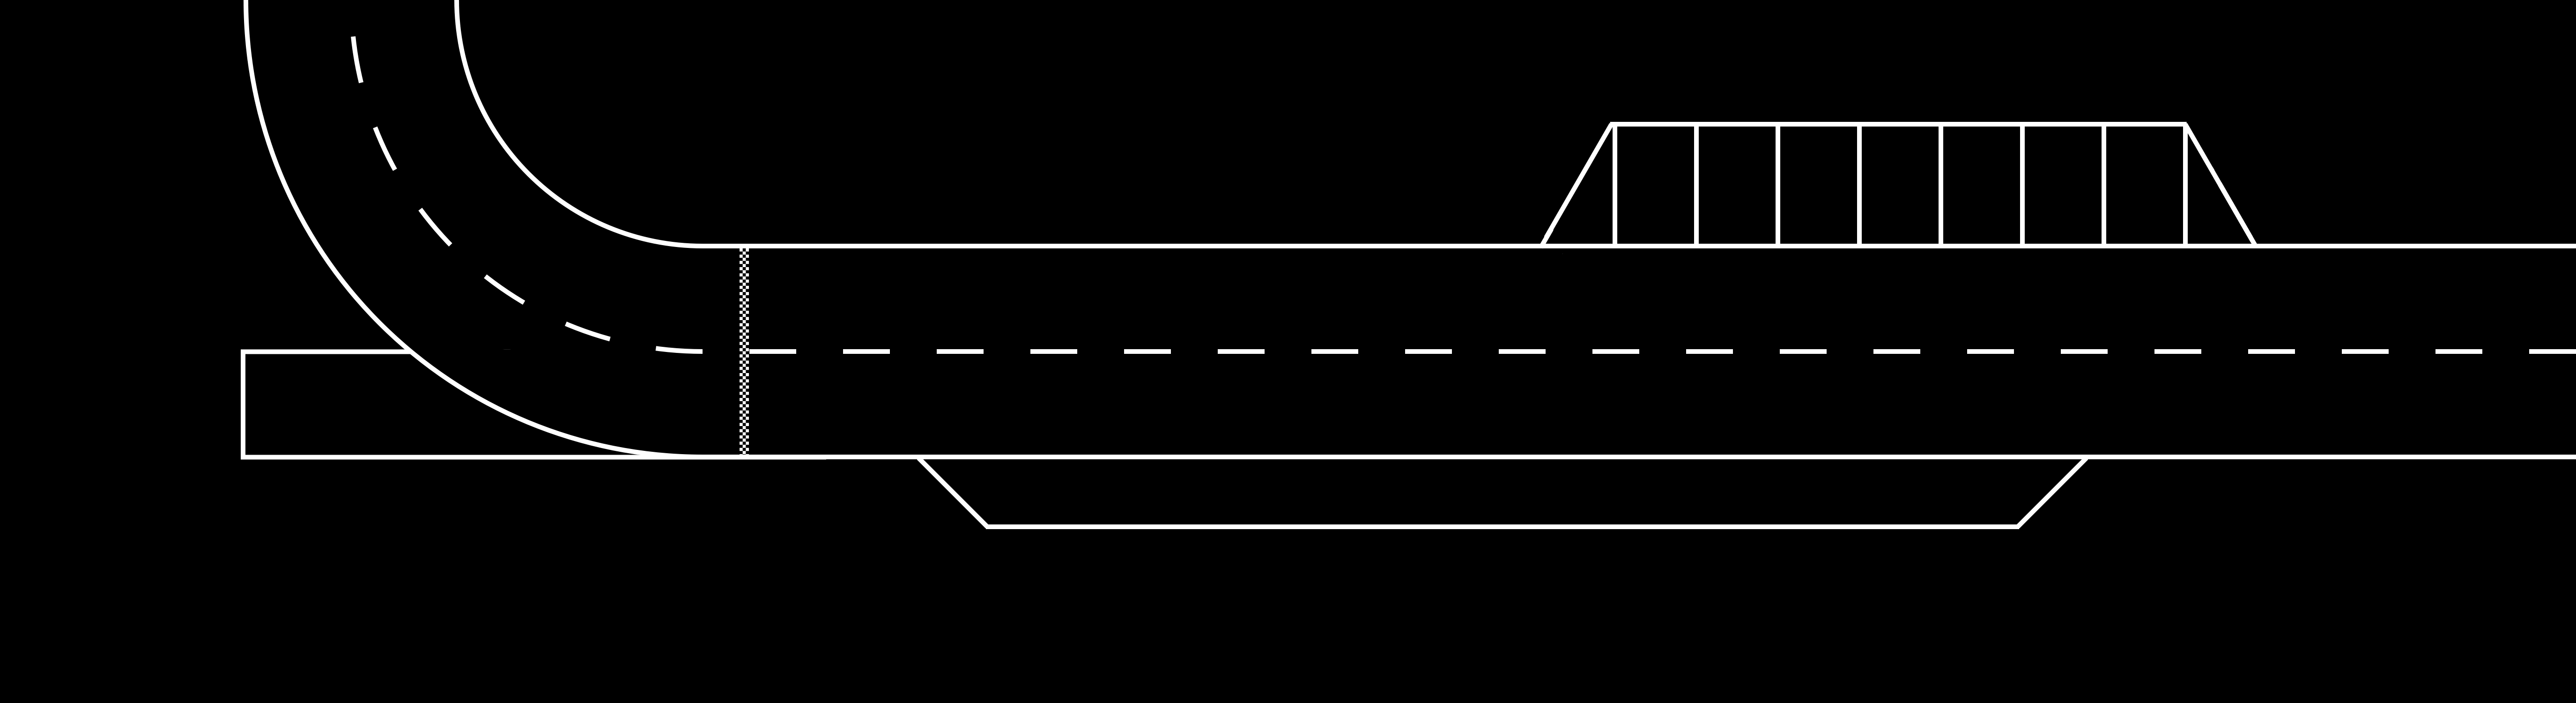
\includegraphics[width=0.7\textwidth]{/home/tb/Desktop/Master/BA_TB/02_Arbeit_Latex/006_Kapitel5/Bilder/start_of_track}% keine extention: w�hlt jpg f�r DVI
  \caption[Startbox- und Parkbereichsegment]%
           {\label{fig:SBPBSegment}%
           Startbox- und Parkbereichsegment}
\end{center}
\end{figure}


\item[] \textbf{Verkehrsinseln}\hfill \\
Die Verkehrsinseln wurden aus einzelnen Pycairo-Modulen mit Inkscape zusammengf�hrt.

\begin{figure}[H]
\begin{center}
  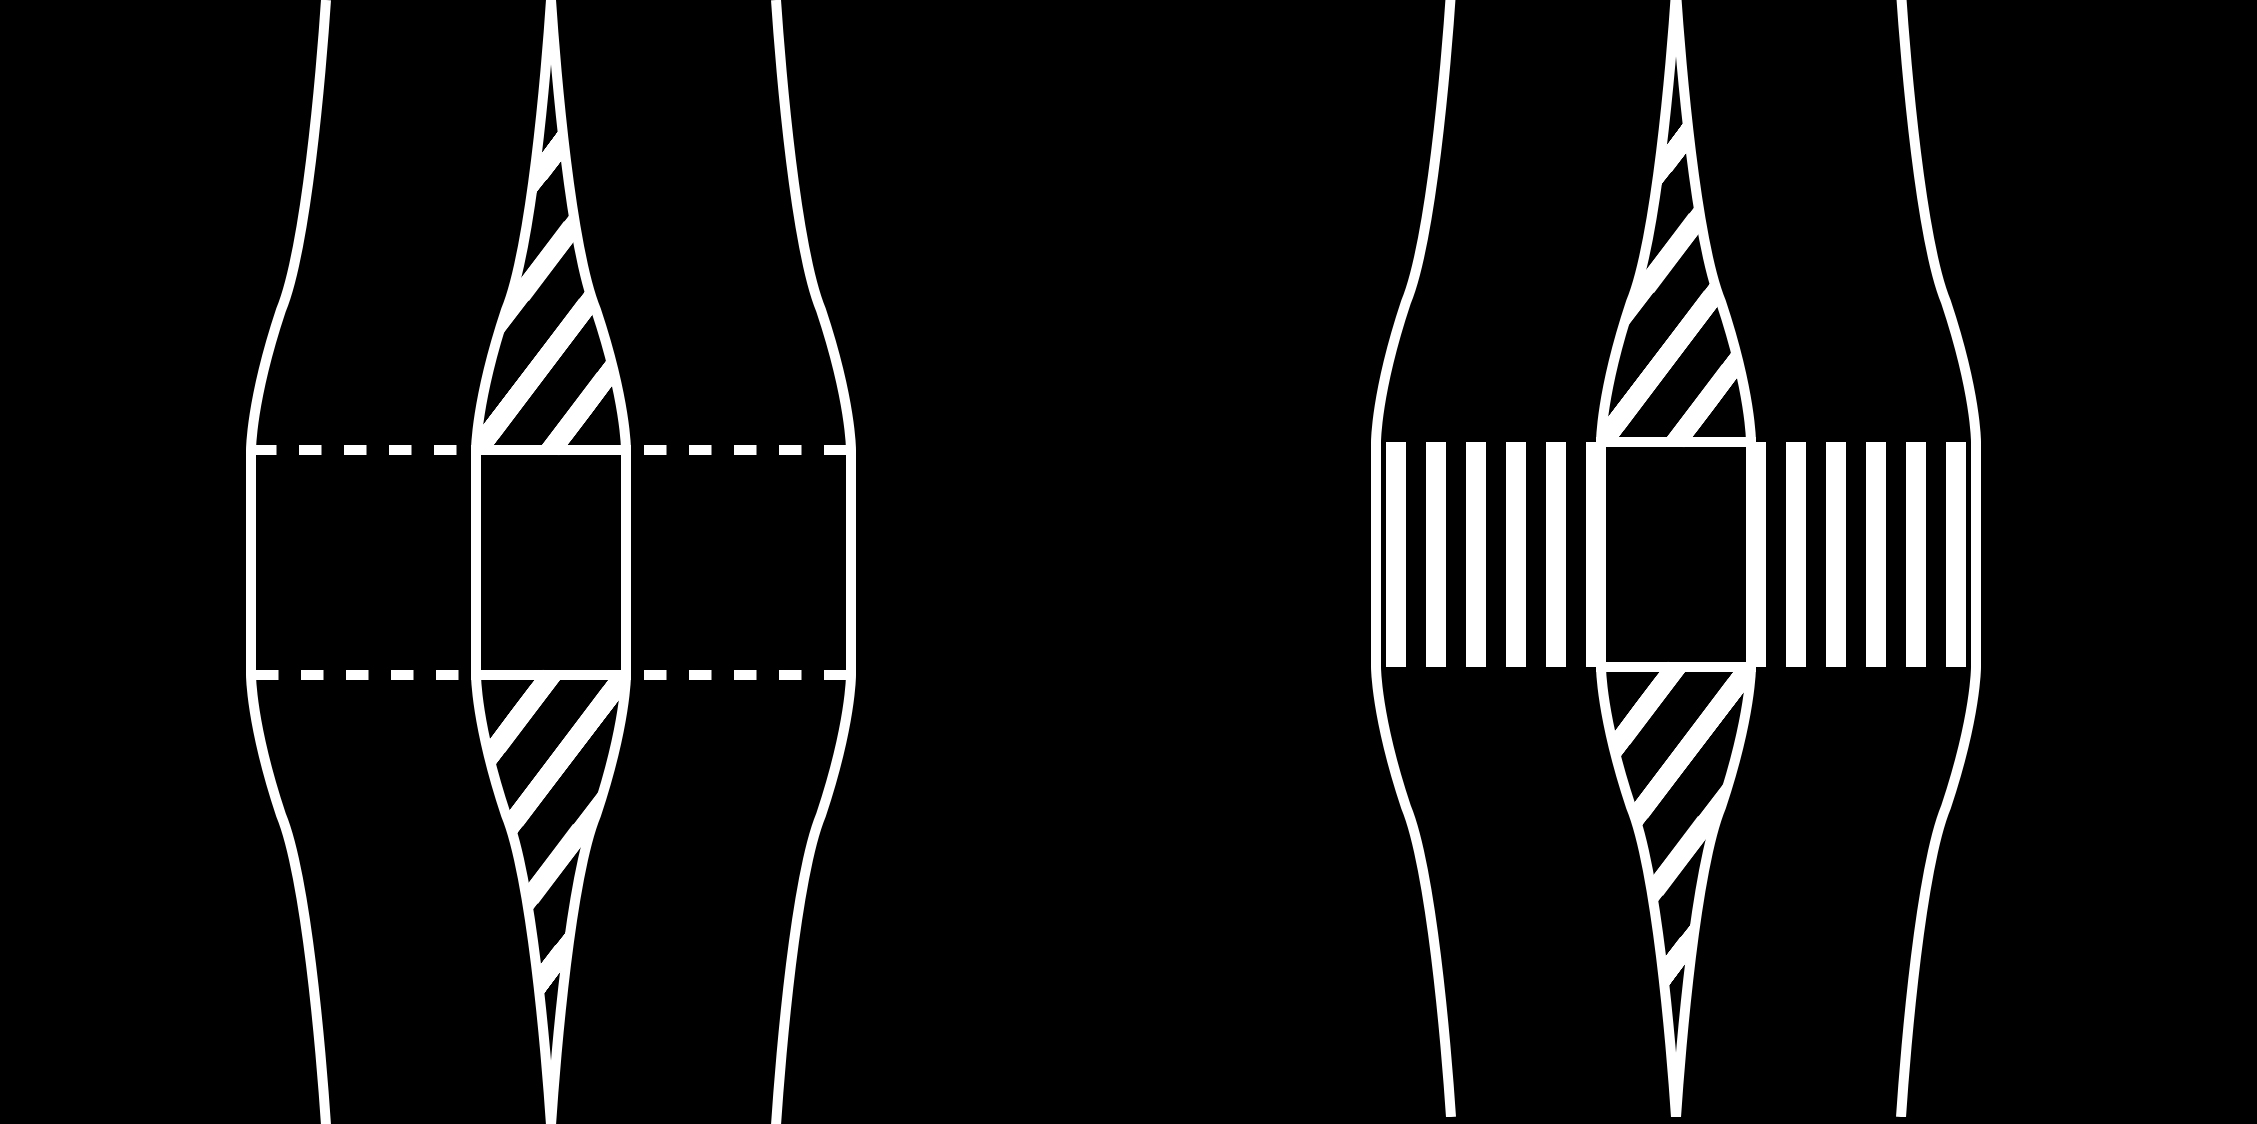
\includegraphics[width=0.5\textwidth]{/home/tb/Desktop/Master/BA_TB/02_Arbeit_Latex/006_Kapitel5/Bilder/islands}% keine extention: w�hlt jpg f�r DVI
  \caption[Verkehrsinselsegmente]%
           {\label{fig:Verkehrsinselsegmente}%
           Verkehrsinselsegmente}
\end{center}
\end{figure}

\item[] \textbf{Linienverdeckungsfl�che}\hfill \\
Es k�nnen schwarze rechteckige Fl�chen erzeugt werden, welche zum Verdecken von Fahrlinien verwendet werden k�nnen. Die Eingangsparameter sind die H�he und Breite der Fl�che.

\item[] \textbf{Verkehrsschilder}\hfill \\
Die im Carolo-Cup m�glichen Verkehrsschilder wurden aus dem Github-Repository von tum-phoenix entnommen \cite{tum}.

\begin{figure}[H]
\begin{center}
  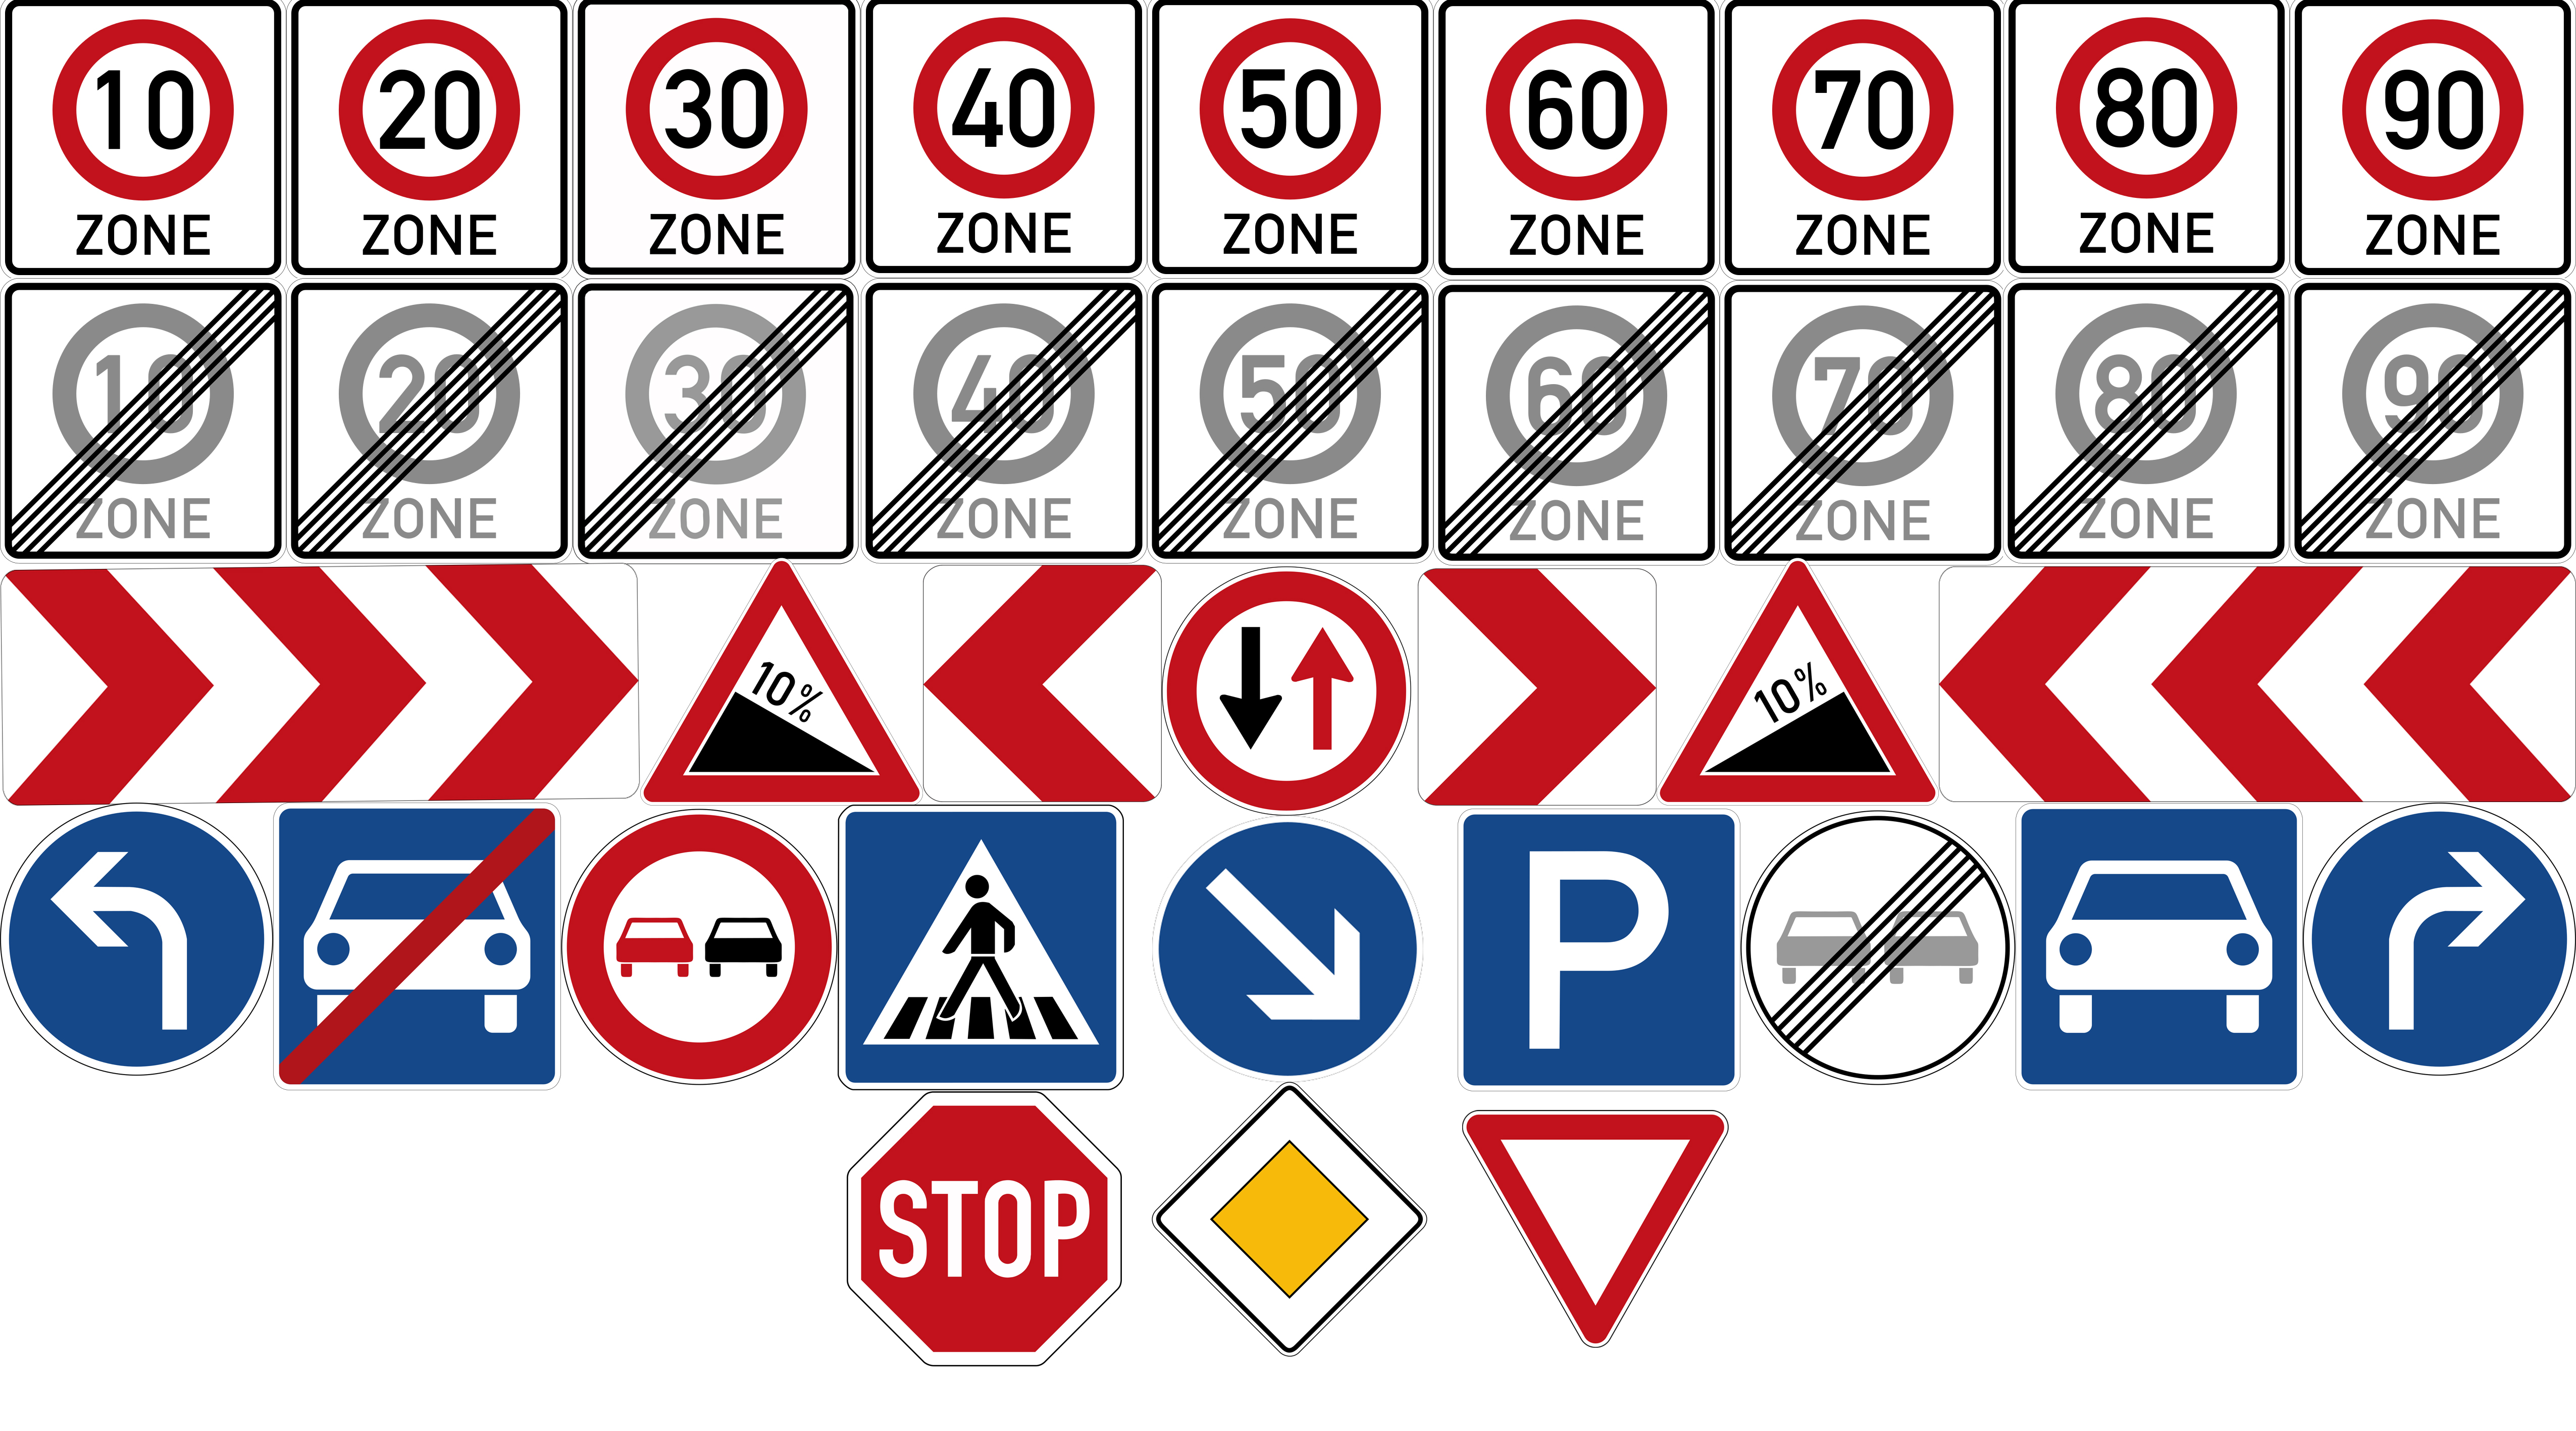
\includegraphics[width=0.7\textwidth]{/home/tb/Desktop/Master/Bilder/alleSchilder}% keine extention: w�hlt jpg f�r DVI
  \caption[Verkehrsschilder des CaroloCups]%
           {\label{fig:Verkehrsschilder}%
           Verkehrsschilder des CaroloCups}
\end{center}
\end{figure}


\item[] \textbf{Abbiegepfeile}\hfill \\
Der Abbiegepfeil wurde dem Github-Repository von tum-phoenix entnommen \cite{tum}.
\end{enumerate}


\begin{figure}[H]
\begin{center}
  
\includegraphics[width=0.1\textwidth]{/home/tb/Desktop/Master/Bilder/abbiegepfeil}% keine extention: w�hlt jpg f�r DVI
  \caption[Abbiegepfeile]%
           {\label{fig:Abbiegepfeile}%
           Abbiegepfeile}
\end{center}
\end{figure}






Das Verh\"altnis an Bildpixeln pro Meter in der Simulationsumgebung wurde dabei in den Python-Skripten auf 500 festgelegt. Dies erm�glicht eine scharfe Ansicht der Module in der Simulationsumgebung, wobei nicht allzu viel Rechenleistung f�r das Rendering ben�tigt wird. Mit dem Python-Skript create\_model\_on\_box k�nnen die Fahrbahn-Module (PNG-Dateien) automatisiert in das Gazebo-Modell-Format (SDF) konvertiert werden.
Daf�r muss der Dateiname, der Speicherort und das Aufl�sungsverh�ltnis als Eingabeparameter dem Skript �bergeben werden. Dieses erzeugt die entsprechende Modell-Datei und kopiert sie in den Gazebo-Modell-Ordner (.gazebo/models). Nach dem Starten des Gazebo-Clients k�nnen die Module im Reiter Insert gefunden und zu einer Fahrbahn zusammengef�hrt werden. 

\begin{figure}[H]
\begin{center}
  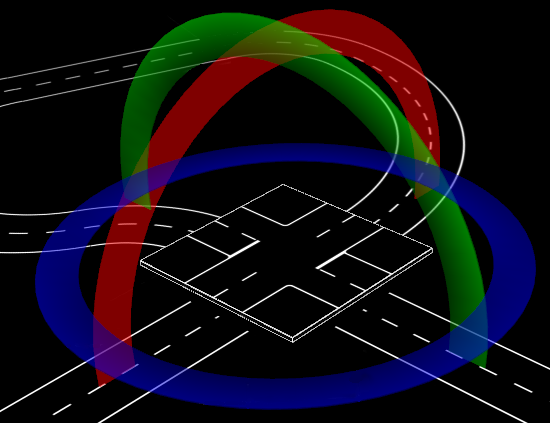
\includegraphics[width=0.5\textwidth]{/home/tb/Desktop/Master/Bilder/rotateFahrbahn}% keine extention: w�hlt jpg f�r DVI
  \caption[ Einf�gen eines Kreuzungssegments in den Gazebo-Simulator]%
           {\label{fig:GazeboKreuzungModel}%
           Einf�gen eines Kreuzungssegments in den Gazebo-Simulator}
\end{center}
\end{figure}


Desweitern k�nnen dreidimensionale Boxen direkt im Gazebo-Client eingef�gt werden. Diese werden zum Beispiel f�r Parkl�cken ben�tigt.

\begin{figure}[H]
\begin{center}
  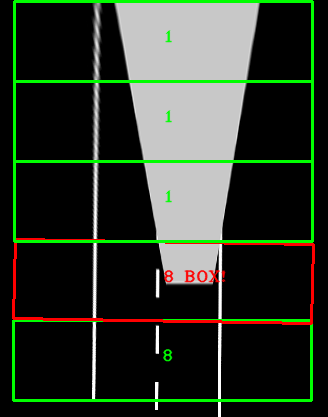
\includegraphics[width=0.5\textwidth]{/home/tb/Desktop/Master/Bilder/box}% keine extention: w�hlt jpg f�r DVI
  \caption[Einf�gen eines Parkl�ckenhindernisses in den Gazebo-Simulator]%
           {\label{fig:GazeboBoxModel}%
           Einf�gen eines Parkl�ckenhindernisses in den Gazebo-Simulator}
\end{center}
\end{figure}

Nach beenden der Fahrbahnmodellierung, kann die Fahrbahn durch den Gazebo-Client als World-Datei im SDF-Format gespeichert werden.

\begin{figure}[H]
\begin{center}
  \includegraphics[width=0.7\textwidth]{/home/tb/Desktop/Master/Bilder/driveTrack}% keine extention: w�hlt jpg f�r DVI
  \caption[Modularer Aufbau eines gesamten Rundkurses im Gazebo-Simulator}]%
           {\label{fig:GazeboRundkursWorld}%
           Modularer Aufbau eines gesamten Rundkurses im Gazebo-Simulator}
\end{center}
\end{figure}



https://github.com/gkouros/ackermann-drive-teleop


\section{Erstellung des Fahrzeugs}
\label{sec:Erstellung der Fahrzeugs}

Die Modellierung des Fahrzeugs wurde mit dem ROS-Package ackermann\_vehicle\_gazebo \cite{ackerm} erm�glicht.
Das Package implementiert ein Fahrzeug mit Ackermann-Lenkung f�r ROS-Gazebo. Daf�r nutzt es das Ackermann-Plugin.
Das Fahrzeug ist durch eine Modell-Datei beschrieben im SDF-Format implementiert. In dieser Modell-Datei wurden Anpassungen vorgenommen, um das Fahrzeug auf die Dimensionen des Fahrzeugs der Hochschule Karlsruhe zu bringen. Au�erdem wurde es um ein Kamera-Plugin erweitert, um Rosbags in der Simulation aufnehmen zu k�nnen. Folgende Parameter lassen sich dar�ber einstellen:

\begin{enumerate}

\item[] \textbf{imageTopicName} \hfill \\
Legt den Namen der Topic fest, auf welche Kamera-Bilder gepublisht werden.

\item[] \textbf{update\_rate} \hfill \\
Legt die Frame-Rate fest in der Bilder auf die Kamera-Topic gepublisht werden.

\item[] \textbf{horizontal\_fov} \hfill \\
Legt den horizontalen Blickwinkel der Kamera fest.

\item[] \textbf{image\_width} \hfill \\
Legt die Bildbreite fest.

\item[] \textbf{image\_height} \hfill \\
Legt die Bildh�he fest.

\item[] \textbf{image\_type} \hfill \\
Legt den Bild-Typ fest (zum Beispiel Graustufenbild).

\item[] \textbf{clip\_near} \hfill \\
Legt die minimale Sichtweite fest.


\item[] \textbf{clip\_far} \hfill \\
Legt die maximale Sichtweite fest

\item[] \textbf{noise\_type} \hfill \\
Legt eine Art von Rauschen auf das Bild (zum Beispiel Gau�sches Rauschen).

\item[] \textbf{noise\_mean} \hfill \\
Legt den Mittelwert des Rauschens fest.

\item[] \textbf{noise\_stddev} \hfill \\
Legt die Standardabweichung des Rauschens fest


\end{enumerate}


Das Steuern des Fahrzeugs ist �ber das ROS-Package joy realisiert. Durch dieses kann das Fahrzeug �ber einen Controller manuell gesteuert werden. In Zukunft k�nnte auch eine autonome Fahrt durch publishen von Fahrinformationen auf die joy-Topic realisiert werden.
�ber Blender wurden zudem die im Wintersemester 18/19 erzeugten CAD-Konstruktionsteile im STL-format zusammengef�hrt. In Blender konnte daraus ein Mesh im Format COLLADA erzeugt werden. COLLADA ist ein XML-basiertes Austausch Format f�r 3D-Programme. Das durch Blender erzeugte Mesh kann zusammen mit dem ackermann\_vehicle\_gazebo-Package genutzt werden um das Carolo-Cup-Fahrzeug in der Simulation darzustellen.


\begin{figure}[H]
\begin{center}
  \includegraphics[width=0.5\textwidth]{/home/tb/Desktop/Master/Bilder/car.png}% keine extention: w�hlt jpg f�r DVI
  \caption[Das in Gazebo simulierte Fahrzeug nach dem vorhandenen CAD-Modell]%
           {\label{fig:GazeboFahrzeug}%
           Das in Gazebo simulierte Fahrzeug nach dem vorhandenen CAD-Modell}
\end{center}
\end{figure}

%
%% Kapitel: Kapitel 4
%%======================================================================

\chapter{Implementierte Bildverarbeitungsalgorithmen}
\label{cha:Implementierte Bildverarbeitungsalgorithmen} \index{Implementierte Bildverarbeitungsalgorithmen}
%


\section{Birdseye-Transformation}
\label{sec:Birdseye-Transformation}

Viele der in dieser Arbeit vewendeten Algorithmen f�hren ihre Berechnungen auf einem in eine andere Perspektive transformierten Bild aus. Dies ist die Birdseye-Perspektive. Sie liefert eine Sicht von oben auf den Fahrbereich. Abstandsmessungen auf der Fahrbahn k�nnen so einfacher implementiert werden. Um das Eingangsbild in die Birdseye-Perspektive zu transformieren, muss eine Transformationsmatrix berechnet werden. Daf�r ben�tigt es der Einstellung der Parameter alpha, beta, gamma der Distanzh�he und der Brennweite, welche mit Hilfe einer grafischen Benutzeroberlf�che realisiert wurde.
Im Folgenden werden die einzelnen Matrizen welche zur Transformation ben�tigt werden beschrieben.

Die Perspektiventransformation von 2D nach 3D:\\
\\
\begin{center}
$ A1 = \left[ \begin{array}{rrr}
1 & 0 & \displaystyle  -\frac{Bildbreite}{2}  \\
\\
0 & 1 & \displaystyle  -\frac{Bildh�he}{2}\\
0 & 0 & 0  \\
0 & 0 & 0 \\
\end{array}\right] $
\end{center}

Die Rotationsmatrix um die X-Achse:\\
\\
\begin{center}
$ R_x = \left[ \begin{array}{rrrr}
1 & 0 & 0 & 0 \\
0 & cos(\alpha) & -sin(\alpha) & 0 \\
0 & sin(\alpha) & cos(\alpha) & 0 \\
0 & 0 & 0 & 1 \\
\end{array}\right] $
\end{center}


Die Rotationsmatrix um die Y-Achse:\\
\\
\begin{center}
$ R_y = \left[ \begin{array}{rrrr}
cos(\beta) & 0 & -sin(\beta) & 0 \\
0 & 1 & 0 & 0 \\
sin(\beta) & 0 & cos(\beta) & 0 \\
0 & 0 & 0 & 1 \\
\end{array}\right] $
\end{center}


Die Rotationsmatrix um die Z-Achse:\\
\\
\begin{center}
$ R_z = \left[ \begin{array}{rrrr}
cos(\gamma) & -sin(\gamma) & 0 & 0 \\
sin(\gamma) & cos(\gamma) & 0 & 0 \\
0 & 0 & 1 & 0 \\
0 & 0 & 0 & 1 \\
\end{array}\right] $
\end{center}



Die Translationsmatrix in der Z-Achse welche einen Zoom erm�glicht:\\
\\
\begin{center}
$ T = \left[ \begin{array}{rrrr}
1 & 0 & 0 & 0 \\
0 & 1 & 0 & 0 \\
0 & 0 & 1 & Distanzh�he \\
0 & 0 & 0 & 1 \\
\end{array}\right] $
\end{center}

Die Perspektiventransformation von 3D nach 2D unter Festlegung der Brennweite:\\
\\
\begin{center}
$ A2 = \left[ \begin{array}{rrrr}
\displaystyle Brennweite & 0 & \displaystyle  -\frac{Bildbreite}{2} & 0 \\
0 & \displaystyle Brennweite &  \displaystyle  -\frac{Bildh�he}{2} & 0 \\
0 & 0 & 1 & 0 \\
\end{array}\right] $
\end{center}

Die Transformationsmatrix berechnet sich nun wie folgt:
\begin{center}
$Transformationsmatrix = A2 \cdot (T \cdot (R_x \cdot R_y \cdot R_z \cdot A1))$ 
\end{center}

Diese Tranformationsmatrix wird als OpenCV-Matrix-Datentyp gespeichert und der Funktion warpPerspective �bergeben welche das Eingangsbild in Birdseye-Perspektive Transformiert.
In folgender Grafik sind die f�r diese Arbeit verwendeten Birdseye-Transformationsparameter mit dem sich daraus ergebenden transformierten Bild dargestellt.

\begin{figure}[H]
\begin{center}
  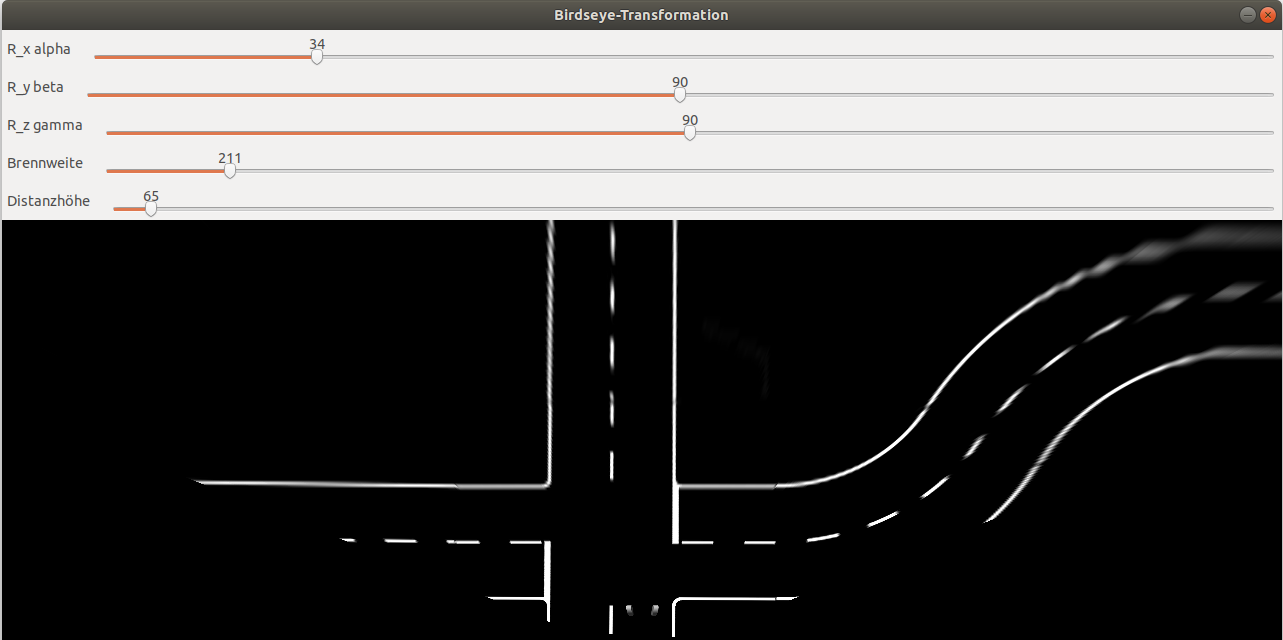
\includegraphics[width=1\textwidth]{/home/tb/gazebo_road_generation/02_Arbeit_Latex/007_Kapitel6/Bilder/birdseyeview}% keine extention: w�hlt jpg f�r DVI
  \caption[GUI zur Anpassung der Birdseye-Transformation]%
           {\label{fig:GUI zur Anpassung der Birdseye-Transformation}%
           GUI zur Anpassung der Birdseye-Transformation}
\end{center}
\end{figure}

Das Verfahren l�sst sich auch einfach durch Verwenden der OpenCV-CUDA-Implementierung parallelisieren, um eine gesteigerte Performanz zu erm�glichen.

%
\section{Startliniensuche mit dem Start-Of-Lines-Search-Algorithmus}
\label{sec:Startliniensuche mit dem Start-Of-Lines-Search-Algorithmus}


Die Startliniensuche sucht im unteren Bildbereich, direkt vor dem Fahrzeug, nach einem eindeutigen Fahrbahnmuster (siehe Abbildung \ref{fig:StartliniensucheFahrbahnmuster}). Der Algorithmus arbeitet auf 
dem Graustufenbild in der Birdseye-Perspektive.
Im ersten Schritt werden drei Bildreihen mit dem horizontalen Abstand HA, nach Pixelintensit�ten �ber einem Schwellwert FS, vom linken zum rechten Bildrand in einer Schleife, abgesucht. Dies geschieht durch einen Filter F, mit der Dimension 1 $\times$ Filterbreite und Schrittweite SW. Die Filterbreite FB muss eine ungerade Zahl sein, wodurch die Mitte des iterierenden Filters als FI bezeichnet ist. Wird eine Pixelintensit�t gr��er FS in F gefunden, so wird in einem mit nullen initialisierten Vector-Container FC der Dimension 1 $\times$ Bildbreite,  der Wert des Vector-Containers auf der Indexposition FI auf eins gesetzt. Es ergeben sich drei Vector-Container mit den entsprechenden Filterantworten auf die jeweilige Bildzeile.
Durch das Absuchen mit dem Filter sollen zusammengeh�rige Liniensegmente besser auffindbar werden falls Fehlstellen in den Linien vorhanden sind. Im darauffolgenden Schritt werden benachbarte Filterantworten zu einem gemeinsamen Segment, definiert durch Segmentbreite und dem Startindex in FC, zusammengef�hrt.
Werden in der mittleren Zeile nicht mindestens drei Segmente gefunden terminiert der Algorithmus.
Werden mehr als zwei Mittelliniensegmente gefunden, wird die Segmentbreite der gefundenen Liniensegmente �berpr�ft. Liegt ein Segment nicht zwischen einem minimalen und maximalen Linienbreiten-Schwellwert wird dieses verworfen. 
Alle Segmente je FC werden anschlie�end untereinander darauf �berpr�ft ob ihr Abstand, dem der Fahrbahnbreite entspricht. Es werden alle Segmente verworfen, welche diesem Kriterium, mit einer festgelegten Toleranz, nicht entsprechen. Die anderen, werden als zusammengeh�rig in einem Vector-Container vermerkt.
Es folgt die �berpr�fung ob die Segmente der einzelnen FC eine gemeinsame Ausrichtung haben. Daf�r wird die Distanz in X-Richtung,
eines Segments eines FC, mit den Segmenten der anderen FC verglichen.
Alle Segmente die keinen Nachbarn mit selber Ausrichtung in einer Toleranzgrenze besitzen, werden verworfen. 
Die �brig gebliebenen zusammengeh�rigen FC Segmente, werden nun darauf �berpr�ft ob zwischen ihnen ein Mittellinien-Segment liegt.
Es darf nur in der mittleren Zeile ein Mittellinien-Segment gefunden werden. Im n�chsten Schritt wird �berpr�ft ob ein Fahrbahnmuster gefunden wurde, das all diese Kriterien erf�llt. Falls nicht terminiert der Algorithmus. Ist ein Muster gefunden, wird zus�tzlich �berpr�ft ob das Muster im korrekten Abstand zum Fahrzeug liegt.
Anschlie�end werden die Startpunkte und Startwinkel f�r die Linke und Rechte Au�enlinie berechnet.


\begin{figure}[H]
\begin{center}
  \includegraphics[width=0.5\textwidth]{/home/tb/Desktop/Master/Bilder/sof_muster}% keine extention: w�hlt jpg f�r DVI
  \caption[StartliniensucheFahrbahnmuster]%
           {\label{fig:StartliniensucheFahrbahnmuster}%
           Das zu suchende Fahrbahnmuster des Start-Of-Lines-Search -Algorithmus}
\end{center}
\end{figure}

\newpage

\begin{figure}[H]
\begin{center}
  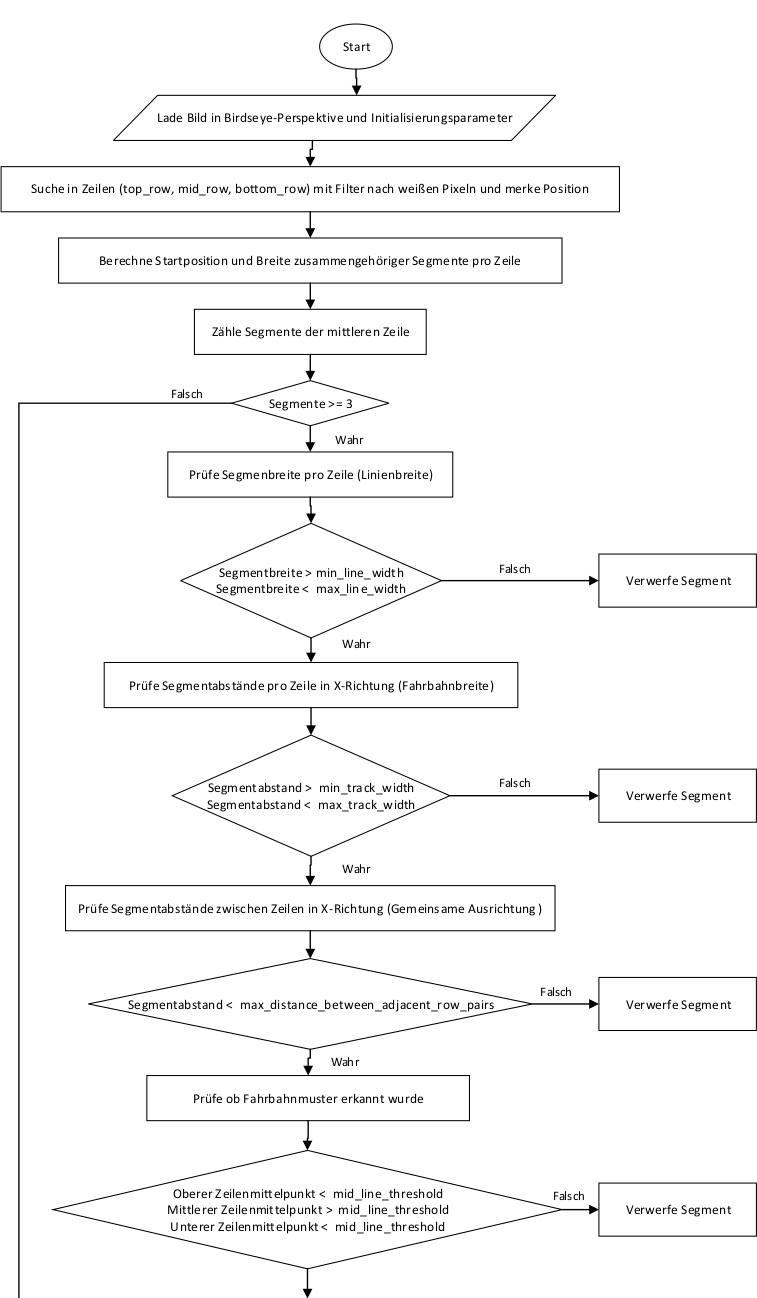
\includegraphics[width=0.8\textwidth]{/home/tb/gazebo_road_generation/02_Arbeit_Latex/007_Kapitel6/Bilder/Start_of_Lines_Diagram_finish1}% keine extention: w�hlt jpg f�r DVI
  \caption[sof1]%
           {\label{fig:sof1}%
           Programmablaufplan des Start-of-Lines-Search-Algorithmus Teil 1}
\end{center}
\end{figure}


\begin{figure}[H]
\begin{center}
  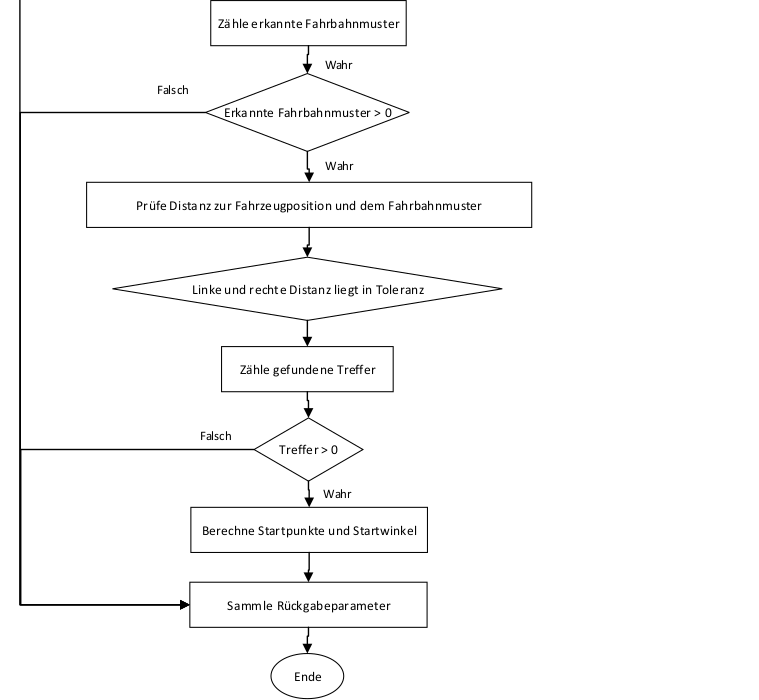
\includegraphics[width=0.8\textwidth]{/home/tb/gazebo_road_generation/02_Arbeit_Latex/007_Kapitel6/Bilder/Start_of_Lines_Diagram_finish2}% keine extention: w�hlt jpg f�r DVI
  \caption[sof2]%
           {\label{fig:sof2}%
           Programmablaufplan des Start-of-Lines-Search-Algorithmus Teil 2}
\end{center}
\end{figure}

\newpage

\section{Startliniensuche mit dem Vanishing-Point-Algorithmus}
\label{sec:Startliniensuche mit dem Vanishing-Point-Algorithmus}

%
%
Der Vanishing-Point-Algorithmus dient dazu sichere Startpunkte der linken und rechten Au�enlinie zu finden. Das Verfahren liefert Punkte mit zugeh�rigem Winkel nahe dem Fahrzeug, nach denen gefahren werden kann. Zudem liefert es Informationen �ber fehlende Au�enlinien.
Der Vanishing-Point-Algorithmus wird auf dem Graustufenbild in Frontalansicht ausgef�hrt.
Der Algorithmus f�hrt die Liniensuche im unteren Bildbereich genau vor dem Fahrzeug aus.
Auf diesen Bildbereich wird zuerst eine Kantenextraktion angewandt.
Dies wird durch den Canny-Edge-Algorithmus erreicht.
Canny nutzt Sobel-Operatoren in X- und Y-Richtung, die mit dem Bild an jeder Position gefaltet werden. Der Operator liefert eine hohe Filterantwort bei einem abrupten �bergang von niedrigen zu hohen Pixelintensit�ten, welche als Kanten wahrgenommen werden. Zudem wird durch die beiden Sobel-Operatoren die Richtung, in welche die Kante zeigt, ermittelt. 
Unter Ber�cksichtigung der Orientierung der Kante, werden lokale Maxima der Filterantwort extrahiert um Kanten�berg�nge auszud�nnen. Die extrahierten Merkmale werden im n�chsten Schritt durch einen Hysterese-Schwellwert gefiltert. Dieser besteht aus zwei Schwellwerten S1 und S2.
Alle Filterantworten, welche unter S1 und S2 liegen werden als Rauschen betrachtet und verworfen. Liegt eine Filterwort �ber S1 und S2 dann ist diese Position eine valide Kante. Werte die zwischen S1 und S2 liegen, werden nur als valide Kanten betrachtet, wenn sie mit Filterantworten verbunden sind, die �ber S1 und S2 liegen. Ansonsten werden diese auch als Rauschen verworfen.

\begin{figure}[H]
\begin{center}
  \includegraphics[width=1\textwidth]{/home/tb/Desktop/Master/Bilder/canny}% keine extention: w�hlt jpg f�r DVI
  \caption[BildbereichCanny]%
           {\label{fig:BildbereichCanny}%
           Darstellung des Bildbereichs nach anwendung des Canny-Edge-Verfahrens}
\end{center}
\end{figure}


Darauf aufbauend, werden durch das Hough-Lines-Algorithmus Linien im Bildbreich gesucht. Durch die Reduktion des Bildbereichs auf relevante Punkte, werden durch Hough-Lines weniger redundante Linien gefunden.
Das Ziel von Hough-Lines ist es Pixel-Gruppen zu finden welche miteinander Linien formen. Hough-Lines transformiert daf�r Pixel, beschrieben durch die Koordinaten X und Y, in einen anderen Merkmals-Raum den Hough-Raum. 
Der Hough-Raum beschreibt alle Geraden, die durch ein Pixel laufen k�nnen �ber die hessesche Normalform: 

$ p = x \cdot cos(\theta) + y \cdot sin(\theta)$

Die neue Ordinate p beschreibt die euklidische Distanz zum Lotfu�punkt. Und die neue Abszisse $\theta$ steht f�r den Winkel zwischen dem Lot der Geraden hin zur Abszisse. Nachdem jedes Pixel des Bildraums in den Hough-Raum transformiert wurde, ergibt sich eine Voting-Matrix deren H�ufigkeitspunkte m�gliche geraden im Bildraum beschreiben. Durch das Setzen eines Schwellwertes, werden nur geraden �ber einer gewissen Anzahl von H�ufigkeitspunkten gefunden, welche nach R�cktransformation die zu suchenden Au�enlinien darstellen.

\begin{figure}[H]
\begin{center}
  \includegraphics[width=0.6\textwidth]{/home/tb/Desktop/Master/Bilder/houghraum}% keine extention: w�hlt jpg f�r DVI
  \caption[HoughRaum]%
           {\label{fig:HoughRaum}%
           Die Hough-Transformation}
\end{center}
\end{figure}


Die OpenCV-Funktion Hough-Lines liefert die Anfangs- und Endpunkte der gefundenen Linien zur�ck.
Darauf folgt das Drehen der Linien in die Fahrtrichtung des Fahrzeugs, im Bild.
Nun werden die Linien aussortiert, welche nicht in den Bildbereichen liegen, in denen die Au�enlinien vorkommen. Dabei wird davon ausgegangen, dass sich das Fahrzeug in der rechten Fahrspur befindet. Da der Algorithmus auf der Frontalansicht arbeitet, k�nnen die Hough-Linien weiter durch ihre Winkel validiert werden. Alle Linien im linken und rechten Bereich werden darauf hin �berpr�ft, ob sie zwischen einem minimalen und maximalen Winkel liegen. Falls dies nicht der Fall ist, werden diese auch verworfen.
Wenn nur eine oder keine Au�enlinie aufzufinden ist, terminiert der Algorithmus.
Werden beide Au�enlinien gefunden, wird untersucht ob die linken und rechten Hough-Linien einen gemeinsamen Schnittpunkt haben. Dieser Schnittpunkt wird auch Vanishing-Point genannt und gibt die Fahrtrichtung des Fahrzeugs an.
Es werden alle Permutation von Schnittpunkten der Linien berechnet. Um nun den besten Vanishing-Point zu finden, nach dem gefahren werden kann, wird der Mittelwert und die Standardabweichung der Punkte berechnet.
In einer While-Schleife werden nur Punkte in Betracht gezogen, welche unter einer maximalen Standardabweichung liegen. Aus diesen Punkten wird dann ein neuer Mittelwert berechnet. Liegen keine Punkte unter der maximalen Standardabweichung vor, erh�ht diese sich immer weiter um eins, bis Punkte gefunden werden, aus welchen der neue Mittelwert berechnet werden kann. 
Ist die Berechnung abgeschlossen, terminiert der Algorithmus.

\begin{figure}[H]
\begin{center}
  \includegraphics[width=1\textwidth]{/home/tb/Desktop/Master/Bilder/vanishingPoint}% keine extention: w�hlt jpg f�r DVI
  \caption[HoughLineVP]%
           {\label{fig:HoughLineVP}%
           Veranschaulichung der Hough-Linien-Suche mit dem errechneten Vanishing-Point und dessen Winkel}
\end{center}
\end{figure}
\newpage



\begin{figure}[H]
\begin{center}
  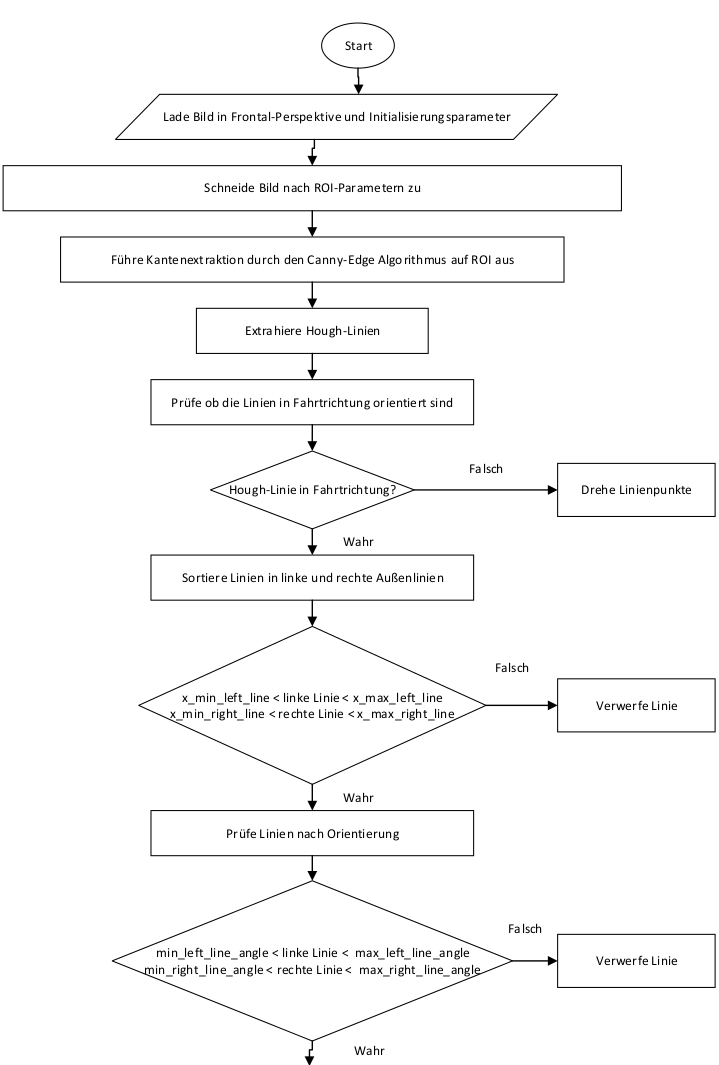
\includegraphics[width=1\textwidth]{/home/tb/gazebo_road_generation/02_Arbeit_Latex/007_Kapitel6/Bilder/vanishing_point_finish1}% keine extention: w�hlt jpg f�r DVI
  \caption[vp1]%
           {\label{fig:vp1}%
           Programmablaufplan des Vanishing-Point-Algorithmus Teil 1}
\end{center}
\end{figure}

\begin{figure}[H]
\begin{center}
  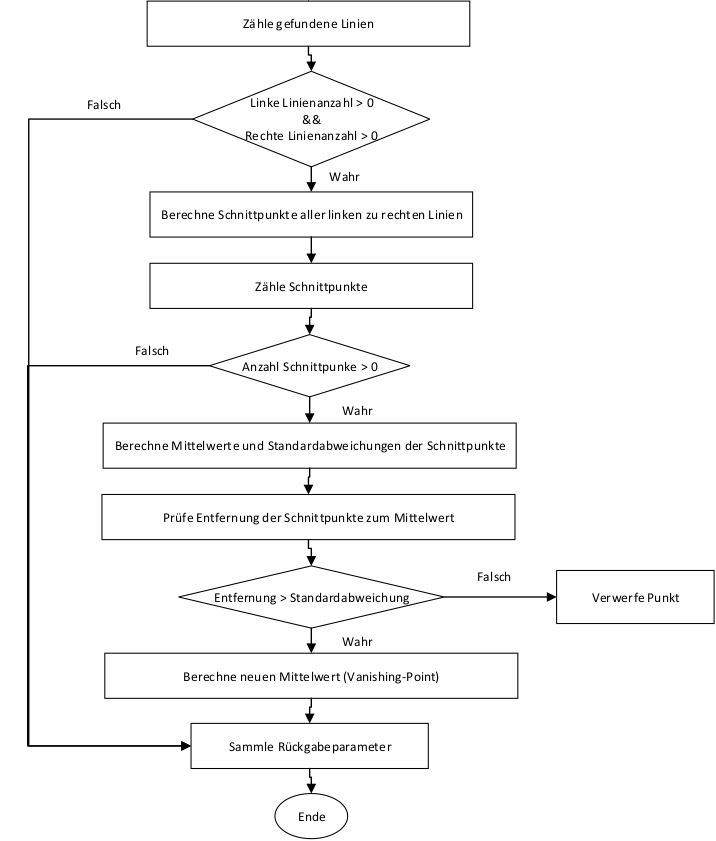
\includegraphics[width=1\textwidth]{/home/tb/gazebo_road_generation/02_Arbeit_Latex/007_Kapitel6/Bilder/vanishing_point_finish2}% keine extention: w�hlt jpg f�r DVI
  \caption[vp2]%
           {\label{fig:vp2}%
           Programmablaufplan des Vanishing-Point-Algorithmus Teil 2}
\end{center}
\end{figure}

\newpage
%
\section{Aussenlinienverfolgung mit dem Line-Follower-Algorithmus}
\label{sec:Aussenlinienverfolgung mit dem Line-Follower-Algorithmus}

Der Line-Follower-Algorithmus setzt auf den beiden Startpunkt-Algorithmen Start-of-Lines-Search-Algorithmus und Vanishin-Point-Algorithmus auf. 
Der Algorithmus arbeitet auf dem Graustufenbild in der Birdseye-Perspektive.
Er ben{\"o}tigt einen Startpunkt und einen Startwinkel als Eingabeparameter. 
Ziel ist es eine Au{\ss}enlinie von einem Startpunkt, im unteren Bildbereich, soweit es m{\"o}glich ist nachzuverfolgen. Das Verfahren ist ein rekursives Verfahren und ruft sich mit neuem Startpunkt und Startwinkel immer wieder selbst auf bis, eine von mehreren Terminierungsbedingungen in Kraft tritt. Angefangen vom ersten Startpunkt betrachtet der Algorithmus eine Anzahl von AR Richtungen mit Sichtweite SW und einem Sichtfeld SF, festgelegt durch einen festen Winkel. Die Mitte des Sichtfeldes wird durch den Startwinkel festgelegt.

\begin{figure}[H]
\begin{center}
  \includegraphics[width=0.5\textwidth]{/home/tb/Desktop/Master/Bilder/line_follower_directions}% keine extention: w�hlt jpg f�r DVI
  \caption[SuchrichtingLF]%
           {\label{fig:SuchrichtingLF}%
           Die AR Suchrichtungen in gelb und t{\"u}rkis und das Sichtfeld des Line-Follower-Algorithmus dargestellt in rot.}
\end{center}
\end{figure}


Im ersten Schritt werden alle Pixelintensit{\"a}ten unter den Zweigen der Suchrichtungen in einem Vector-Container gesammelt.
Anschlie{\ss}end wird der Algorithmus Otsus-Methode auf diesen Container angewandt.
Otsus-Methode findet einen Schwellwert der das Bild in zwei Klassen aufteilt.
In diesem Fall der schwarze Hintergrund der Fahrbahn und die wei{\ss}en Linien.
Es wird ein Histogramm aus vorkommenden Pixel-Intensit{\"a}ten erzeugt und ein Schwellwert berechnet, der die gewichtete Interklassen Varianz der beiden Klassen minimiert. Mit dem berechneten Otsu-Schwellwert werden die AR Suchrichtungen wieder durchschritten. F{\"u}r jede der Suchrichtungen wird die aktuelle Intensit{\"a}t der Position mit dem Otsu-Schwellwert verglichen. Liegt eine Intensit{\"a}t unter dem Otsu-Schwellwert wird die vorherige Position und die Akkumulation aller Pixel-Intensit{\"a}ten bis zu dieser Position gespeichert. Ansonsten bricht die Suche nach Erreichen von SW in dem derzeitigen Zweig ab und es wird auch hier die Positionen mit akkumulierten Pixel-Intensit{\"a}ten gespeichert.
Sind alle Zweige durchlaufen wird {\"u}ber all jene der nach Intensit{\"a}ten gewichtete Schwerpunkt ermittelt.
Das Pixel im Vierer-Nachbarschaftsbereich des Schwerpunktes mit h{\"o}chster Intensit{\"a}t wird als neuer Startpunkt festgelegt. Und der neue Suchwinkel ist der Winkel zwischen altem und neuem Startpunkt. Der Algorithmus ruft die Suchfunktion erneut auf bis eines der folgenden Terminierungsbedingungen erf{\"u}llt ist. 


\begin{enumerate}

\item[] \textbf{Eine maximale Anzahl von Iterationen wurde erreicht} \hfill \\
\item[] \textbf{Der Suchpunkt ist au{\ss}erhalb des Bildbereichs} \hfill \\

\item[] \textbf{Die Suche bleibt Stecken} \hfill \\
Wenn gefundene Punkte, nacheinander, sich unter einer festgelegten euklidischen Distanz zum vorhergehenden Punkt befinden, wird ein Counter hochgesetzt welcher den rekursiven Aufruf terminiert wenn dieser Counter einen Schwellwert {\"u}berschreitet.

\item[] \textbf{Die Suche bewegt sich zur{\"u}ck} \hfill \\
Wenn der Y-Wert des vorherigen Startpunktes gr{\"o}{\ss}er ist als der neue Startpunkt, wird eine Counter erh{\"o}ht der nach {\"u}berschreiten eines Schwellwertes den Algorithmus terminiert.

\end{enumerate}


\begin{figure}[H]
\begin{center}
  \includegraphics[width=0.5\textwidth]{/home/tb/Desktop/Master/Bilder/linefollower}% keine extention: w�hlt jpg f�r DVI
  \caption[LPLF]%
           {\label{fig:LPLF}%
           Die gefundenen Linienpunkte des Line-Follower-Algorithmus f�r die linke(gelb) und rechte(t{\"u}rkis Au�enlinie)}
\end{center}
\end{figure}

\newpage

\begin{figure}[H]
\begin{center}
  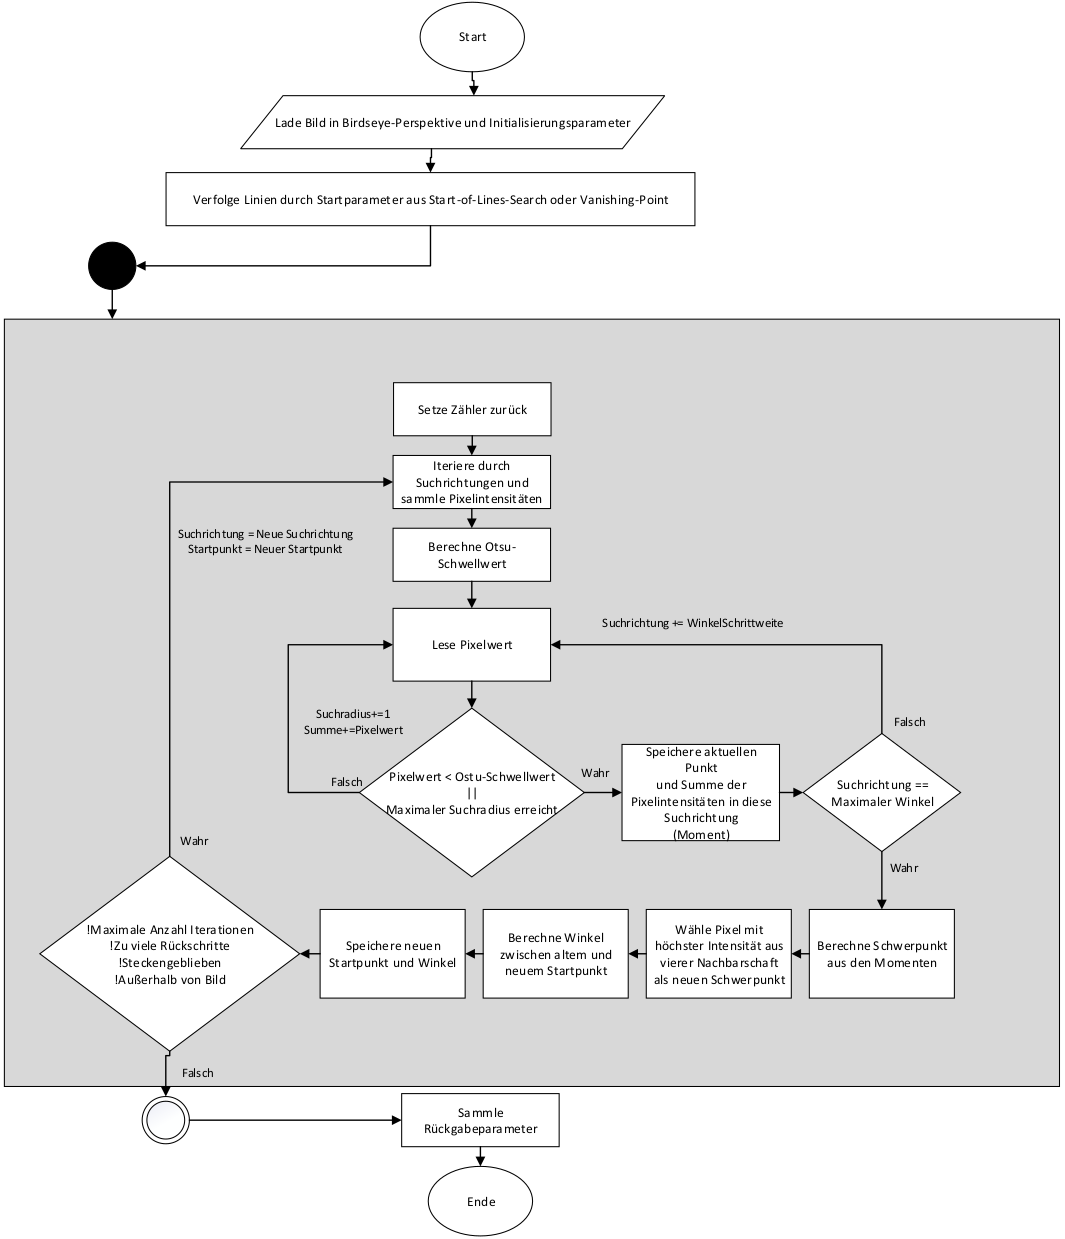
\includegraphics[width=1\textwidth]{/home/tb/gazebo_road_generation/02_Arbeit_Latex/007_Kapitel6/Bilder/Line_Follower_Diagram_finish1}% keine extention: w�hlt jpg f�r DVI
  \caption[linefollowpa]%
           {\label{fig:linefollowpa}%
           Programmablauf des Line-Follower-Algorithmus)}
\end{center}
\end{figure}


\newpage


\section{Linienpunktereduzierung mit dem Line-Points-Reducer-Algorithmus}
\label{sec:Linienpunktereduzierung mit dem Line-Points-Reducer-Algorithmus}

%
Der Douglas-Peucker-Algorithmus kann verwendet werden um eine Polylinie durch Reduzierung der Anzahl der enthaltenen Punkte ann{\"a}hrend zu beschreiben.
Da der Line-Follower-Algorithmus viele nah beieinander liegende Punkte findet, welche keine wichtigen Informationen enthalten, werden diese durch den Douglas-Peucker-Algorithmus verworfen um nur noch auf den wichtigen Punkten arbeiten zu k{\"o}nnen.
Dies geschieht durch das Legen einer imagin{\"a}ren Linie zwischen dem ersten und dem letzten Punkt in einer Reihe von Punkten, welche die Polylinie bilden. Es wird gepr{\"u}ft, welcher Punkt am weitesten von dieser Linie entfernt ist. Die Entfernung ist die euklidische Distanz des Punktes zu dessen Lotfu{\ss}punkt auf der Linie. Wenn der gefundene Punkt (und wie folgt alle anderen Zwischenpunkte) eine kleinere euklidische Distanz als ein gegebener Abstand Epsilon besitzt, werden alle dazwischen liegenden Punkte entfernt. Wenn dieser Ausrei{\ss}er-Punkt andererseits weiter von der Linie entfernt ist als Epsilon, wird die Polylinie in zwei Teile geteilt. Zum einen vom ersten Punkt bis einschlie{\ss}lich zum Ausrei{\ss}er-Punkt. Zum anderen vom Ausrei{\ss}er-Punkt bis hin zum Endpunkt.

\begin{figure}[H]
\begin{center}
  \includegraphics[width=0.4\textwidth]{/home/tb/Desktop/Master/Bilder/Douglas_Peucker}% keine extention: w�hlt jpg f�r DVI
  \caption[RDPAlgorihtmus]%
           {\label{fig:RDPAlgorihtmus}%
           Veranschaulichung des Douglas-Peucker-Algorithmus}
\end{center}
\end{figure}




Die Funktion wird f{\"u}r beide resultierenden Polylinien rekursiv aufgerufen.
Der Start- und Endpunkt wie alle Ausrei{\ss}er-Punkte ergeben die neue reduzierte Linie.

\begin{figure}[H]
\begin{center}
  \includegraphics[width=0.4\textwidth]{/home/tb/Desktop/Master/Bilder/rdp}% keine extention: w�hlt jpg f�r DVI
  \caption[RDPAlgorihtmusBild]%
           {\label{fig:RDPAlgorihtmusBild}%
           Darstellung der Linienpunkte nach der anwendung des Douglas-Peucker-Algorithmus}
\end{center}
\end{figure}


Der Algorithmus gibt als R{\"u}ckgabewert die reduzierten Linien-Punkte des Line-Follower-Algorithmus zur{\"u}ck. Jeder Punkt tr{\"a}gt als zus{\"a}tzliche Information den Winkel und die Distanz zu seinem n{\"a}chsten Nachbarpunkt.

\newpage

\section{Mittelliniensuche und Grapherzeugung mit dem Mid-Line-Search-Algorithmus}
\label{sec:Mittelliniensuche und Grapherzeugung mit dem Mid-Line-Search-Algorithmus}

%
%
Um eine robuste Linienerkennung zu erm{\"o}glichen muss auch die Mittellinie in betracht gezogen werden. Der Algorithmus nutzt dabei einen Clustering-Ansatz. Zuerst werden einzelne Pixel, die zu einer Mittellinie geh{\"o}ren in einer Gruppe zusammengef{\"u}hrt. Anschlie{\ss}end werden aufeinanderfolgende Mittellinien-Gruppen, wenn sie unter einem gewissen Abstand voneinander entfernt sind, zu Knoten in einem Graphen vereint. Der Algorithmus startet mit dem Einlesen des Graustufenbilds in Birdseye-Perspektive.
Das Eingangsbild wird in Raster der H{\"o}he RH und der Breite RB aufgeteilt. Die einzelnen Bereiche stehen f{\"u}r Gruppen durch welche Mittellinien gekennzeichnet sind. Jeder Bildbereich wird dadurch mit einen Bereichsschl{\"u}ssel gekennzeichnet. Der Schl{\"u}ssel ist ein Tupel definiert durch pair<int,int>. Die einzelnen Bereichsschl{\"u}ssel sind abh{\"a}nig von der Bilddimension und der Rasterisierung.
Der Schl{\"u}ssel eines Bereichs wird beschrieben durch:

$\displaystyle \frac{Bildh{\"o}he}{RH}$ (erster Wert des Tupels)  
 
$\displaystyle \frac{Bildbreite}{RB}$ (zweiter Wert des Tupels).


\begin{figure}[H]
\begin{center}
  \includegraphics[width=0.7\textwidth]{/home/tb/Desktop/Master/Bilder/rasterierung_small}% keine extention: w�hlt jpg f�r DVI
  \caption[RasterisiertesBild]%
           {\label{fig:RasteriertesBild}%
           Das Rasterisierte Bild in rot mit zugeh�rigen Rasterschk�sseln in gr�n}
\end{center}
\end{figure}  

\newpage

Durch eine For-Schleife wird durch das Bild iteriert und die Pixelintensit{\"a}ten PI werden mit dem festgelegten Schwellwert PIS verglichen. Wird ein PI gr{\"o}{\ss}er PIS auf einer Pixelposition PP gefunden so wird die Funktion radial\_scan aufgerufen. Die Funktion sucht in einem Radius SR alle PI um PP ab. Wird eine PI gefunden die gr{\"o}{\ss}er als ein maximaler radialer Schwellwert MRS ist, dann bricht der Algorithmus ab und geht zur n{\"a}chsten PP {\"u}ber. Falls keiner der PI um die PP gr{\"o}{\ss}er dem MRS ist wird diese PP mit ihrem zugeh{\"o}rigen Bereichsschl{\"u}ssel in dem Container multimap<pair<int,int>,Point> gespeichert. Dementsprechend wird das ganze Bild durchlaufen.
Im n{\"a}chsten Schritt wird die Anzahl von PP f{\"u}r jeden Bereichsschl{\"u}ssel im Multimap-Container gez{\"a}hlt. Liegt diese Anzahl unter einem minimalen Schwellwert MPPS so wird der Speicherbereich (PPs mit zugeh{\"o}rigem Bereichsschl{\"u}ssel) aussortiert. Die {\"u}brigbleibenden Daten innerhalb des Multimap-Containers k{\"o}nnen als valide Gruppen von Mittellinienpunkte MP angesehen werden. Falls der Multimap-Container leer ist terminiert der Algorithmus und keine Mittellinien wurden gefunden. Ist die Mittelliniensuche nicht terminiert beginnt der Aufbau eines ungerichteten Graphen.
Im ersten Schritt werden daf{\"u}r die geometrischen Schwerpunkte GS durch die MP f{\"u}r jeden Bereichsschl{\"u}ssel berechnet. Anschlie{\ss}end wird die euklidische Distanz zwischen den GS der Bereichsschl{\"u}ssel mit einem Schwellwert verglichen. Ist die Distanz zweier GS unter dem Schwellwert geh{\"o}ren die Bereichsschl{\"u}ssel I und J zusammen und diese Verbindung wird in einem Vector-Container hinterlegt.  
Alle m{\"o}glichen Permutationen werden so verglichen. Durch die Funktion isPermuted wird w{\"a}hrenddessen sichergestellt das nicht dieselben Bereichsschl{\"u}ssel verglichen werden als auch das keine Bereichsschl{\"u}ssel mehrmals mit dem Schwellwert verglichen werden.
Wurden alle Verbindungen von Bereichsschl{\"u}sseln berechnet, werden diese durch den Algorithmus Depth-First-Search aufgel{\"o}st. Depth-First-Search ist ein rekursiver Algorithmus der angewandt wird um  Knoten in einem Graphen zu suchen. Im Gegensatz zur Breitensuche BFS wird bei der Tiefensuche DFS zun{\"a}chst ein Pfad vollst{\"a}ndig in die Tiefe beschritten, bevor abzweigende Pfade beschritten werden.
DFS wurde gew{\"a}hlt, da die Bereichsschl{\"u}ssel so gut wie immer nur einen Nachbarknoten besitzen und nicht in die Breite gesucht werden muss. Dies ist damit zu begr{\"u}nden das die Mittellinien der Fahrbahn aufeinanderfolgen. Au{\ss}erdem ben{\"o}tigt DFS weniger Speicherressourcen da nicht alle Kind-Knoten eines aktuell zu pr{\"u}fenden Knotens gespeichert werden m{\"u}ssen. Zudem sind die Knoten nach Beendigung der Suche bereits topologisch sortiert. Durch die implementierte Klasse depth\_first\_search werden die Bereichsschl{\"u}ssel zu Graphen zugeordnet. Dabei k{\"o}nnen auch Graphen mit nur einem Knoten entstehen.

\begin{figure}[H]
\begin{center}
  \includegraphics[width=0.8\textwidth]{/home/tb/Desktop/Master/Bilder/midlinesearch_cluster}% keine extention: w�hlt jpg f�r DVI
  \caption[MittellinienGraph]%
           {\label{fig:MittellinienGraph}%
           Darstellung eines Graphen von verbundenen Mittellinien.
           Der gr�ne Punkt und der rote Kreis geben die Start und Endwerte der einzelnen Mittelliniensegmente an.
           }
\end{center}
\end{figure}  

Ist DFS terminiert werden die in den Graphen enthaltenen Bereichsschl{\"u}ssel durch den Abstand ihres GS zum Fahrzeug sortiert. Dies ist durch die Funktion sort realisiert, welche durch {\"U}berladung mit einer Lambda-Funktion nach der kleinsten euklidischen Distanz absteigend zum Fahrzeug hin sortiert. Werden keine Graphen mit einer Anzahl Knoten gr{\"o}{\ss}er eins gefunden, terminiert der Algorithmus. Ist dies nicht der Fall, werden zus{\"a}tzlich der Richtungswinkel und der Abstand eines Knoten zu seinem n{\"a}chsten Nachbarn berechnet.

\newpage

\begin{figure}[H]
\begin{center}
  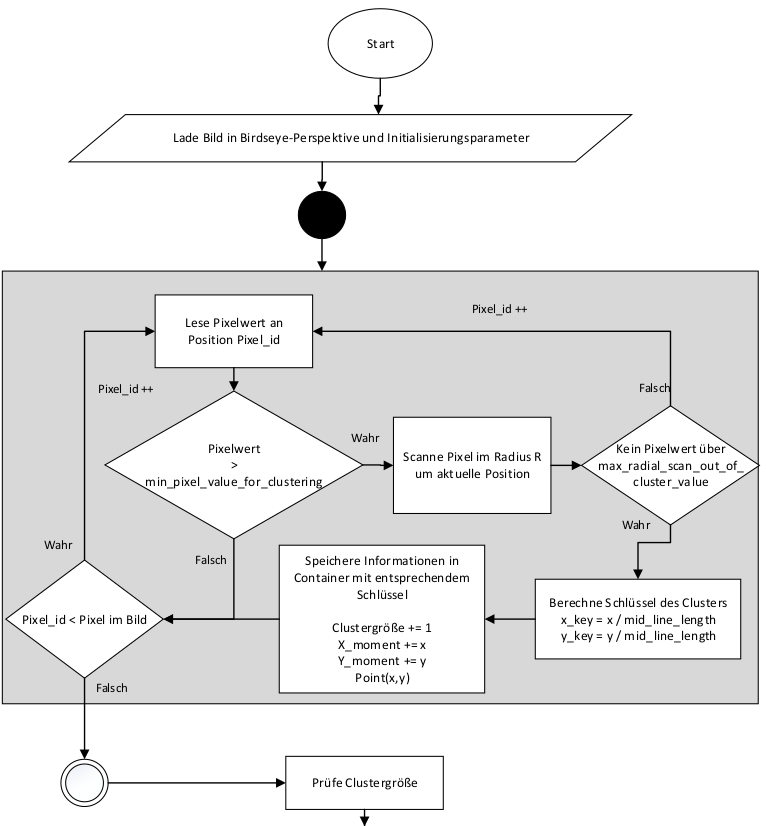
\includegraphics[width=1\textwidth]{/home/tb/gazebo_road_generation/02_Arbeit_Latex/007_Kapitel6/Bilder/Mid_Line_Search_Diagram1}% keine extention: w�hlt jpg f�r DVI
  \caption[midlinepa1]%
           {\label{fig:midlinepa1}%
           Programmablaufplan des Mid-Line-Search-Algorithmus Teil 1.
           }
\end{center}
\end{figure} 

\begin{figure}[H]
\begin{center}
  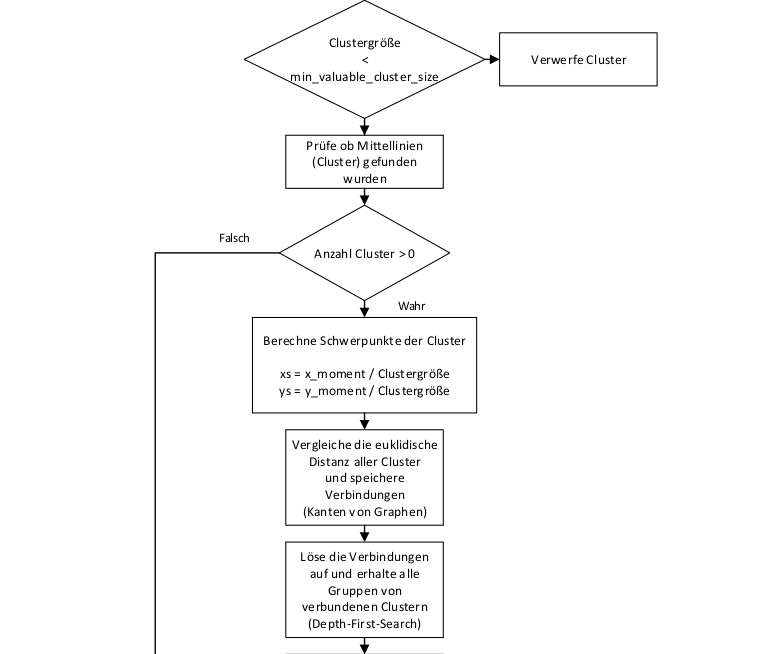
\includegraphics[width=1\textwidth]{/home/tb/gazebo_road_generation/02_Arbeit_Latex/007_Kapitel6/Bilder/Mid_Line_Search_Diagram2}% keine extention: w�hlt jpg f�r DVI
  \caption[midlinepa2]%
           {\label{fig:midlinepa2}%
           Programmablaufplan des Mid-Line-Search-Algorithmus Teil 2.
           }
\end{center}
\end{figure} 


\begin{figure}[H]
\begin{center}
  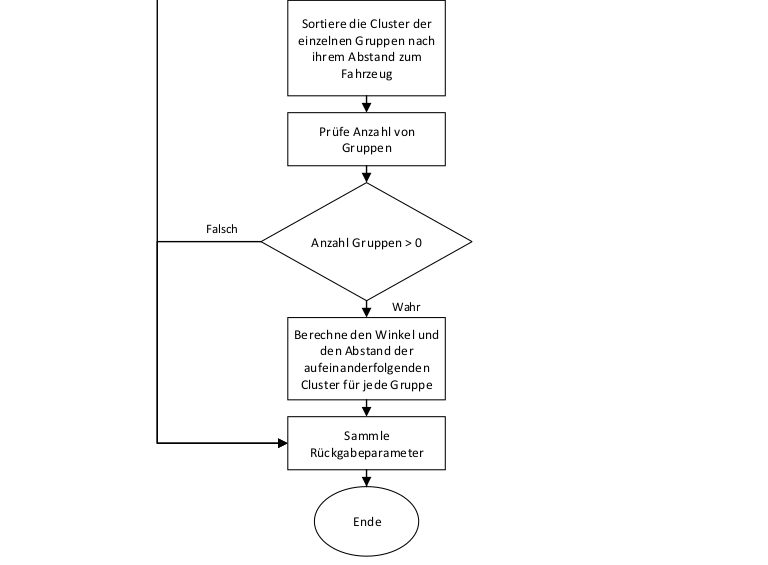
\includegraphics[width=1\textwidth]{/home/tb/gazebo_road_generation/02_Arbeit_Latex/007_Kapitel6/Bilder/Mid_Line_Search_Diagram3}% keine extention: w�hlt jpg f�r DVI
  \caption[midlinepa3]%
           {\label{fig:midlinepa3}%
           Programmablaufplan des Mid-Line-Search-Algorithmus Teil 3.
           }
\end{center}
\end{figure} 



%https://stackoverflow.com/questions/3332947/when-is-it-practical-to-use-depth-first-search-dfs-vs-breadth-first-search-bf
%Comparing BFS and DFS, the big advantage of DFS is that it has much lower memory requirements than BFS, because it?s not necessary to %store all of the child pointers at each level.

\newpage

\section{Bewertungstabellenerzeugung mit dem Line-Validation-Table-Creator-Algorithmus}
\label{sec:Bewertungstabellenerzeugung mit dem Line-Validation-Table-Creator-Algorithmus}

%
%
Der Line-Validation-Table-Creator-Algorithmus erzeugt eine Bewertungstabelle aus den zur{\"u}ckgelieferten Werten des Line-Points-Reducer-Algorithmus und Mid-Line-Search-Algorithmus. Diese Werte sind Punkte mit einer zugeh{\"o}rigen Richtung der L{\"a}nge zum n{\"a}chsten Punkt auf der entsprechenden Linie. 
In der Bewertungstabelle werden Informationen {\"u}ber einzelne Punkte der gefundenen Linken-, Mittel- und Rechten-Linie-Punkte berechnet, vermerkt und verglichen um eine robuste Linienerkennung zu erm{\"o}glichen. Daf{\"u}r wird zuerst das Graustufenbild in Birdseye-Perspektive an den Algorithmus {\"u}bergeben, auf welchem Line-Validation-Table-Creator seine Berechnungen ausf{\"u}hrt. Anschlie{\ss}end werden die einzelnen Linien {\"u}bergeben. Mit den Folgenden Enumerationen welche als Schl{\"u}sselvariablen dienen kann bestimmt werden welche Linien verglichen werden sollen. Gleichzeitig werden dadurch auch Variablen an die entsprechenden Linien angepasst.


\begin{enumerate}

\item[] \textbf{LEFT\_TO\_MID} \hfill \\
Suchrichtung von der linken Linie zur Mittellinie.

\item[] \textbf{LEFT\_TO\_RIGHT} \hfill \\
Suchrichtung von der linken Linie zur rechten Linie.

\item[] \textbf{MID\_TO\_LEFT} \hfill \\
Suchrichtung von der Mittellinie zur linken Linie.

\item[] \textbf{MID\_TO\_RIGHT} \hfill \\
Suchrichtung von der Mittellinie zur rechten Linie.

\item[] \textbf{RIGHT\_TO\_LEFT} \hfill \\
Suchrichtung von der rechten Linie zu linken Linie.

\item[] \textbf{RIGHT\_TO\_MID} \hfill \\
Suchrichtung von der revchten Linie zur linken Linie.

\end{enumerate}


Eine weitere gesetzte Konvention ist, das die Linien von links (LEFT\_LINE = 0) nach rechts (RIGHT\_LINE = 2) durchnummeriert sind.

Je nach Schl{\"u}ssel-Variable wird eine Linie abh{\"a}ngig von den Parametern - Richtung und L{\"a}nge, zum n{\"a}chsten Punkt durchschritten. Dabei werden f{\"u}r jeden Punkt , orthogonal zu diesem, Liniensegmente auf benachbarten Linien im Graustufenbild gesucht. Der orthogonale Suchwinkel ist abh{\"a}ngig von der Schl{\"u}ssel-Variable und der Richtung zum n{\"a}chsten Punkt der aktuellen Linie. Wird ein valides Segment gefunden (seine Breite liegt zwischen einem minimalen und maximalen Schwellwert), wird dies in einer Klasse vermerkt. Diese Klasse ist die Line-Validation-Table-Klasse. Jeder Punkt einer Linie ist somit eine eigene Klasse in der verschiedene Informationen vermerkt, wie auch Getter- und Setter-Funktionen implementiert sind. Wurden alle Linien-Punkte f{\"u}r jede Linie durchlaufen, werden die erzeugten Informationen, untereinander verglichen. Dadurch wird jeder Linien-Punkt (Line-Validation-Table-Klasse) mit weiteren Informationen bef{\"u}llt.
Es wird {\"u}berpr{\"u}ft ob f{\"u}r einen gefundenen benachbarten Linien-Punkt aus dem Graustufenbild, ein Punkt in den benachbarten Bewertungstabellen gefunden wird der sehr nah zu diesem liegt. Daf{\"u}r wird die minimale euklidische Distanz der Punkte gesucht. Liegt diese unter einem Schwellwert wird ein Flag in der entsprechenden Bewertungstabelle gesetzt. Dies soll der Absicherung der Punkte dienen. Des Weiteren wird die Richtung der einzelnen Punkte untereinander auf ihre gleiche Ausrichtung hin {\"u}berpr{\"u}ft, um f{\"u}r einen noch h{\"o}here Genauigkeit zu sorgen.
Da die Mittellinien in einem Vector-Container bestehend aus einem Vector-Container mit zusammengeh{\"o}rigen Mittellinien-Gruppen gespeichert sind, werden Mittellinien-Punkte einer anderen Gruppe in der Line-Validation-Table-Klasse mit einer zus{\"a}tzlichen Identifikationsnummer markiert.
 
\begin{figure}[H]
\begin{center}
  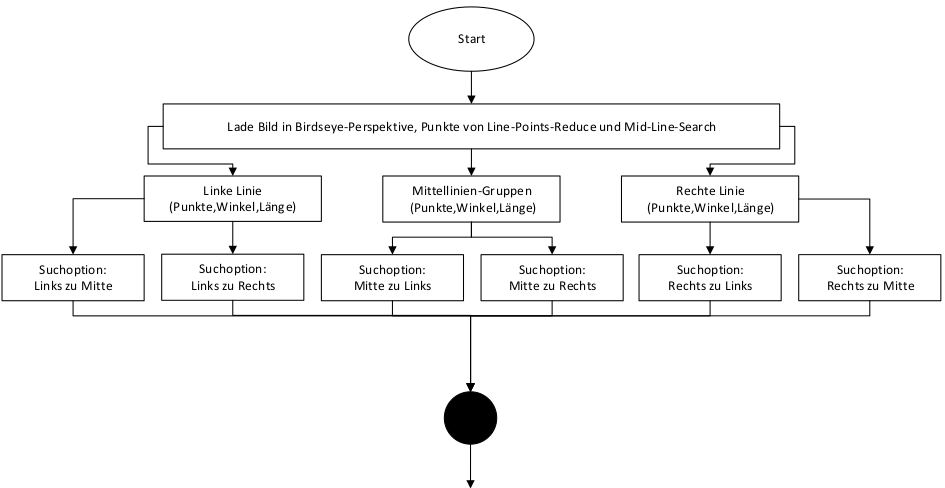
\includegraphics[width=1\textwidth]{/home/tb/gazebo_road_generation/02_Arbeit_Latex/007_Kapitel6/Bilder/Line_Validation_Table_finish1}% keine extention: w�hlt jpg f�r DVI
  \caption[lvtc1]%
           {\label{fig:lvtc1}%
           Programmablaufplan der Line-Validation-Table-Creator-Algorithmus Teil 1.
           }
\end{center}
\end{figure}
 
 \newpage
 
\begin{figure}[H]
\begin{center}
  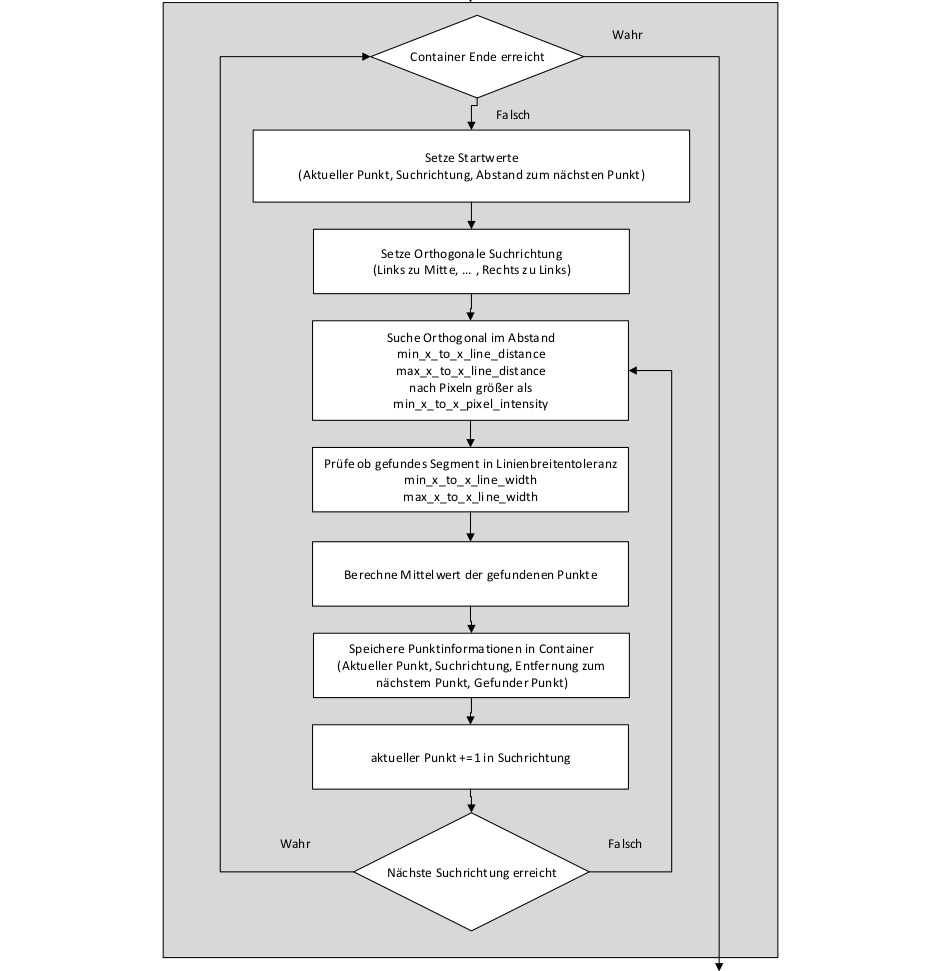
\includegraphics[width=1\textwidth]{/home/tb/gazebo_road_generation/02_Arbeit_Latex/007_Kapitel6/Bilder/Line_Validation_Table_finish2}% keine extention: w�hlt jpg f�r DVI
  \caption[lvtc2]%
           {\label{fig:lvtc2}%
           Programmablaufplan der Line-Validation-Table-Creator-Algorithmus Teil 2.
           }
\end{center}
\end{figure}
 
\newpage 
 
\begin{figure}[H]
\begin{center}
  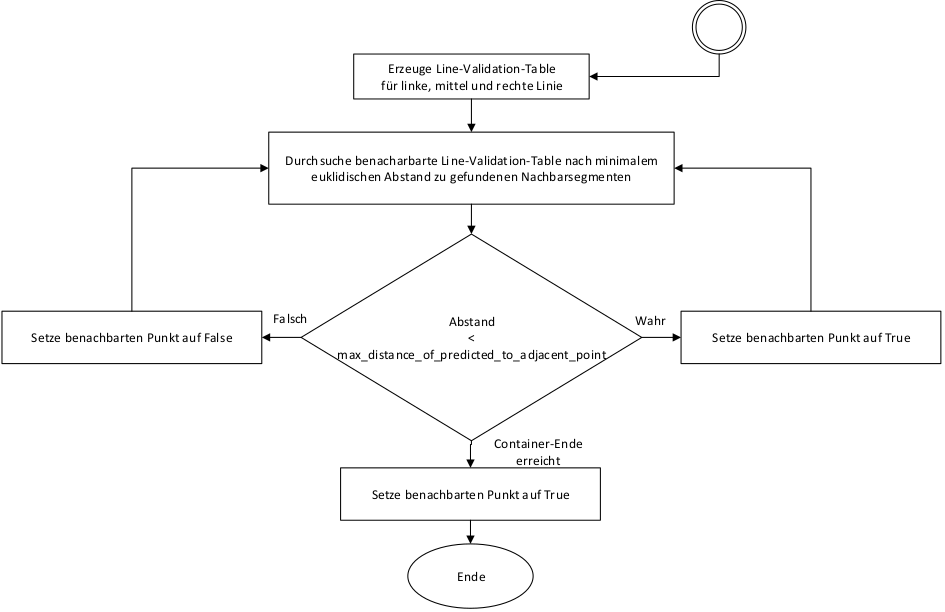
\includegraphics[width=1\textwidth]{/home/tb/gazebo_road_generation/02_Arbeit_Latex/007_Kapitel6/Bilder/Line_Validation_Table_finish3}% keine extention: w�hlt jpg f�r DVI
  \caption[lvtc3]%
           {\label{fig:lvtc3}%
           Programmablaufplan der Line-Validation-Table-Creator-Algorithmus Teil 3.
           }
\end{center}
\end{figure}
 
\newpage

Mit der Funktion GetDrivePointsInDriveDirection k�nnen aus der Line-Validation-Table-Creator-Klasse Punkte extrahiert werden, welche in Fahrtrichtung verlaufen. Abzweigungen wie sie bei Kreuzungen entstehen werden nicht ber{\"u}cksichtigt.
Die Funktion betrachtet dabei die {\"A}nderung des Winkels zwischen den einzelnen Punkten einer Linie. Dazu muss der Startwinkel an welchem die Linie im unteren Bildbereich beginnt zwischen einem minimalen und maximalen Schwellwert liegen, damit die Linie ber{\"u}cksichtigt wird. Anschlie{\"ss}end wird durch die Linien-Punkte der Bewertungstabellen iteriert und die Winkel{\"a}nderung der Punkte verglichen. Bei einer abrupten {\"A}nderung {\"u}ber einem Schwellwert wird die Linie abgeschnitten und als Return-Wert ausgegeben. Der Datentyp ist dabei immernoch vector<LineValidationTable> mit allen gespeicherten Informationen.

\begin{figure}[H]
\begin{center}
  \includegraphics[width=0.5\textwidth]{/home/tb/Desktop/Master/Bilder/indrivedir}% keine extention: w�hlt jpg f�r DVI
  \caption[ExtrahierteLinienpunkte]%
           {\label{fig:ExtrahierteLinienpunkte}%
           Extrahierte linke(gelb), mittel(lila) und rechte(t{\"u}rkis) Linienpunkte in Fahrtrichtung.
           }
\end{center}
\end{figure}

\newpage

\section{Sicherheitsbewertung der Fahrbahnbereiche durch den Safe-Drive-Area-Evaluator-Algorithmus}
\label{sec:Sicherheitsbewertung der Fahrbahnbereiche durch den Safe-Drive-Area-Evaluator-Algorithmus}

%
%
Der Safe-Drive-Area-Evaluator-Algorithmus dient zur Sicherheitsbewertung von befahrbaren Fahrbahnbereichen.
Diese rechteckigen Bereiche werden von unten nach oben im Bild fortlaufend ausgewertet.
Der Algorithmus f{\"u}hrt seine Berechnung auf dem Graustufenbild in Birdseye-Perspektive aus.
Der Algorithmus verwendet die aus der Line-Validation-Table-Creator-Klasse extrahierten Fahrbahninformationen in Fahrtrichtung.
Im ersten Schritt wird ein Rechteck mit der Dimension SafteyRectWidth $\times$ SafetyRectHeight im Bildbereich vor dem Fahrzeug betrachtet.
Mit der OpenCV-Funktion PolygonTest kann ein Punkt darauf gepr{\"u}ft werden ob er sich in einem Polygon befindet. Dieses Polygon ist in diesem Fall das Rechteck. Die linken, mittel und rechten Bewertungstabellen-Punkte in Fahrtrichtung werden darauf gepr{\"u}ft ob sie im derzeit betrachteten Rechteck liegen. Anschlie{\ss}end wird eine Metrik erzeugt, welche die Sicherheit des Bereichs kompakt in einer Zahl bewertet. Daf{\"u}r werden die im aktuellen Rechteck enthaltenen Bewertungstabellen-Punkte aller Linien ausgewertet. Im Folgenden sind die Informationen erl{\"a}utert, welche zur Erzeugung der Metrik genutzt werden. Dabei sind sie der Priorit{\"a}t nach absteigend geordnet.

\begin{enumerate}

\item[] \textbf{Priorit{\"a}t 0} \hfill \\
Ein Bewertungstabellen-Punkt hat beide benachbarten Segmente gefunden und die benachbarten Bewertungstabellen besitzen je einen Punkt in der N{\"a}he dieser.

\item[] \textbf{Priorit{\"a}t 1 und 2} \hfill \\
Ein Bewertungstabellen-Punkt hat beide benachbarten Segmente gefunden und eine benachbarte Bewertungstabelle besitzt einen Punkt in der N{\"a}he dessen.

\item[] \textbf{Priorit{\"a}t 3 und 4} \hfill \\
Ein Bewertungstabellen-Punkt hat ein benachbartes Segment gefunden und die benachbarte Bewertungstabelle besitzt einen Punkt in der N{\"a}he dessen.

\item[] \textbf{Priorit{\"a}t 5} \hfill \\
Ein Bewertungstabellen-Punkt hat beide benachbarten Segmente gefunden aber keine benachbarte Bewertungstabelle besitzt einen Punkt in der N{\"a}he dessen.

\item[] \textbf{Priorit{\"a}t 6 und 7} \hfill \\
Ein Bewertungstabellen-Punkt findet ein benachbartes Segment

\end{enumerate}



Um eine kompakte Beschreibung der Bereichssicherheit zu erm{\"o}glichen, werden die Priorit{\"a}ten der Bewertungstabellen-Punkte aller Linien im Rechteck akkumuliert. Des Weiteren wird die Anzahl der Priorit{\"a}ten in einen prozentualen Wert umgewandelt. Dieser prozentuale Wert ist im normalen Fall abh{\"a}ngig von der H{\"o}he des Rechtecks. Dieser beschreibt wieviele Punkte maximal im Rechteck liegen k{\"o}nnen. Da jedoch bei einer Kurvenfahrt theoretisch mehr Punkte als SafetyRectHeight im Rechteck vorkommen k{\"o}nnen, wird in diesem Ausnahmefall die Anzahl der Bewertungstabellen-Punkte im Rechteck verwendet. Die prozentualen Werte f{\"u}r jede der akkumulierten Priorit{\"a}ten werden anschlie{\ss}end zu einem Wert zusammengef{\"u}hrt.



\begin{center}


\begin{tabular}{|c|c|c|c|c|c|c|c|}


\textbf{P 0} & \textbf{P 1} & \textbf{P 2} & \textbf{P 3} & \textbf{P 4} & \textbf{P 5} & \textbf{P 6} & \textbf{P 7}\\
\hline
0-99\% &  0-99\% &  0-99\% &    0-99\% &   0-99\% &   0-99\% &   0-99\% &   0-99\%    


\end{tabular}

\end{center}



Die Berechnung dient nur zur kompakten Beschreibung der Bereichssicherheit in einer maximal zehnstelligen gro�en Zahl, damit sie als einzelner Wert an Funktionen {\"u}bergeben und einfach interpretiert werden kann. Dieser Wert beschreibt die Sicherheit der Punkte im ersten Rechteck. In der 
Darauf aufbauend, werden nun die sichersten Bewertungstabellen-Punkte aus dem Rechteck verwendet um die Richtung zu erhalten, in welche die Fahrspur ausgerichtet ist. Vom Mittelpunkt des derzeitig betrachteten Rechtecks wird in die berechnete Richtung mit einer festgelegten Schrittweite vorangeschritten und die n{\"a}chste Bereichssicherheit berechnet.
Falls in einem Bereich keine Bewertungstabellen-Punkte mit oben beschriebenen Priorit{\"a}tswerten vorhanden sind, wird im Winkel des vorherigen Rechtecks solange vorangeschritten, bis der Mittelpunkt eine Rechtecks au{\ss}erhalb des betrachteten Graustufenbilds liegt. 

\begin{figure}[H]
\begin{center}
  \includegraphics[width=0.5\textwidth]{/home/tb/Desktop/Master/Bilder/safetytrack2}% keine extention: w�hlt jpg f�r DVI
  \caption[RectSafety]%
           {\label{fig:RectSafety}%
           Bewertete Bereichssicherheiten dargestellt als gr�ne Rechtecke.
           Die als gr�ne Zahl dargestellte Sicherheitsbewertung gibt die Anzahl von dezimalstellen der Bewertung im Bereich an.
           }
\end{center}
\end{figure}



Dies erlaubt es zus{\"a}tzlich {\"u}ber Kreuzungen hinaus, Bereiche fr{\"u}hzeitig zu bewerten.

\begin{figure}[H]
\begin{center}
  \includegraphics[width=0.5\textwidth]{/home/tb/Desktop/Master/Bilder/safetytrack}% keine extention: w�hlt jpg f�r DVI
  \caption[SafetyRectKreuzung]%
           {\label{fig:SafetyRectKreuzung}%
           Bewertung der Bereichssicherheit �ber die Kreuzung hinaus.
           }
\end{center}
\end{figure}

Wurden alle m{\"o}glichen Bereiche ausgewertet terminiert die Funktion und gibt die Bereichsicherheiten zur{\"u}ck.



%
%% Kapitel: Kapitel 4
%%======================================================================

\chapter{Suche von Bodenmarkierungen und Objekten in den Fahrspuren}
\label{cha:Suche von Bodenmarkierungen und Objekten in den Fahrspuren}
\index{Suche und Klassifizierung von Bodenmarkierungen und Objekten in den Fahrspuren}
%
%
In folgenden Abschnitten wird auf die entwickelten Verfahren zur Erkennung von Bodenmarkierungen und von Objekten in der Fahrbahn und der Startbox eingegangen.

\section{Startboxschrankenerkennung}
\label{sec:Startboxschrankenerkennung}

Die Startboxschrankenerkennung nutzt die Softwarebibliothek Zbar.
Zbar ist eine Open-Source-Bibliothek zum Lesen von C-Barcodes und QR-Codes.
Es wurde sich dazu entschieden den QR-Code der Startboxschranke zu erkennen, da dieser nur einmal auf der gesamten Fahrstrecke vorkommt. Zbar ist rechenintensiv jedoch kann der Algorithmus einfach nach dem �ffnen der Schranke ausgeschalten werden und f�llt dadurch nicht mehr ins Gewicht.
Um das Erkennen der Startboxschranke testen zu k�nnen, wurde mit Qt/QML eine Grafische Benutzeroberfl�che implementiert.

\begin{figure}[H]
\begin{center}
  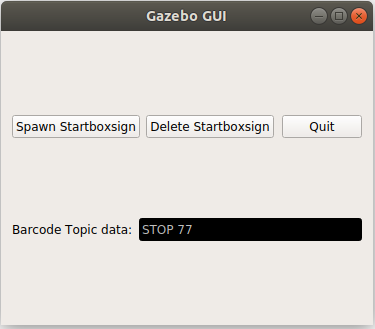
\includegraphics[width=0.5\textwidth]{/home/tb/gazebo_road_generation/02_Arbeit_Latex/008_Kapitel7/Bilder/gui}% keine extention: w�hlt jpg f�r DVI
  \caption[Grafische Benutzeroberfl�che]%
           {\label{fig:Grafische Benutzeroberfl�che}%
           Grafische Benutzeroberfl�che f�r das Testen der Startboxschrankenerkennung}
\end{center}
\end{figure}

Mit dieser kann das Modell der Startboxschranke in der Simulation erzeugt und wieder gel�scht werden.
Au�erdem besitzt die GUI einen Subscriber auf die QR-Code-Topic barcode und zeigt bei Erkennen der Startboxschranke in der GUI den erkannten Text an.
Um daf�r zu sorgen, dass die GUI nicht einfriert und jederzeit auf Signale reagieren kann, wurde die GUI in einem separaten Thread nebenl�ufig zu ROS implementiert.

\begin{figure}[H]
\begin{center}
  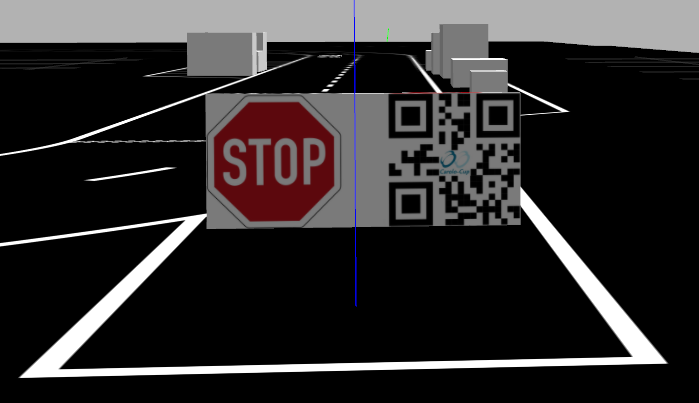
\includegraphics[width=0.5\textwidth]{/home/tb/gazebo_road_generation/02_Arbeit_Latex/008_Kapitel7/Bilder/startbox}% keine extention: w�hlt jpg f�r DVI
  \caption[Startboxschranke]%
           {\label{fig:Startboxschranke}%
           Die erzeugte Startboxschranke.}
\end{center}
\end{figure}


\section{Zebrastreifen- und Ziellinienerkennung}
\label{sec:Zebrastreifen- und Ziellinienerkennung}

Um Zebrastreifen und Ziellinien im aktuellen Bild zu erkennen, wird nach einer festgelegten Anzahl von aufeinanderfolgenden wei�en und schwarzen Pixelsegmenten mit einer definierten breite gesucht.
Das Verfahren arbeitet auf dem Graustufenbild in der Birdseye-Perspektive.
Der Algorithmus setzt dabei auf die Startparameter des Start-of-Lines-Search-Algorithmus oder des Vanishing-Point-Algorithmus auf. Die Startparameter von Start-of-Lines-Search werden dabei pr�feriert.
Es wird eine zu vorausschauende Distanz und eine Schrittweite definiert, in der vor dem Fahrzeug nach dem Muster der Fahrbahnmarkierungen gesucht wird.
Die Zebrastreifensuche iteriert orthogonal zu dem Startwinkel aus Startparameters. Daf�r wird die OpenCV-Funktion Lineiterator genutzt.
Diese iteriert von einem Startpunkt hin zu einem Endpunkt durch das Bild und liest die darunter liegenden Pixel aus. Wird eine gewisse Anzahl wei�er und schwarzer Segmente mit der entsprechenden Breite gefunden, ist der Zebrastreifen erkannt.

\begin{figure}[H]
\begin{center}
  
\includegraphics[width=0.4\textwidth]{/home/tb/gazebo_road_generation/02_Arbeit_Latex/008_Kapitel7/Bilder/crosswalk}% keine extention: w�hlt jpg f�r DVI
  \caption[Zebrastreifensuche]%
           {\label{fig:Zebrastreifensuche}%
           Ein detektierter Zebrastreifen in der Fahrbahn.}
\end{center}
\end{figure}

Die Ziellinienerkennung sucht von der linken Au�enlinie orthogonal zu dem Startwinkel von Startparameters nach Segmenten mit der entsprechenden Breite. Auch sie nutzt die OpenCV-Funktion Lineiterator.
Da die Ziellinie im CaroloCup h�ufig nach einer Kurve erkannt werden muss, wird ein Sichtfeld durch einen Winkel definiert, welches durch wiederholtes Aufrufen von Lineiterator in einer festgelegten Schrittweite durchsucht wird. 

\begin{figure}[H]
\begin{center}
  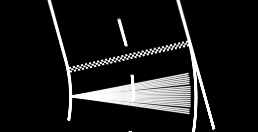
\includegraphics[width=0.5\textwidth]{/home/tb/gazebo_road_generation/02_Arbeit_Latex/008_Kapitel7/Bilder/goalline_search}% keine extention: w�hlt jpg f�r DVI
  \caption[Zielliniensuche]%
           {\label{fig:Zielliniensuche}%
           Darstellung des Sichtfelds der Zielliniensuche.}
\end{center}
\end{figure}

\begin{figure}[H]
\begin{center}
  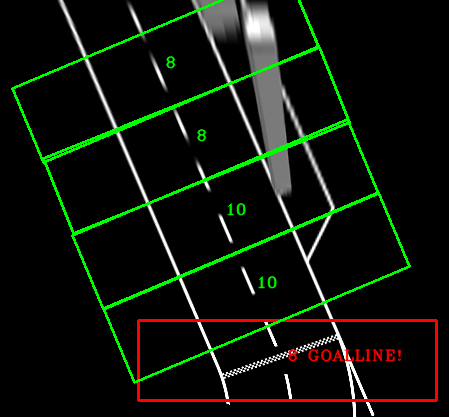
\includegraphics[width=0.4\textwidth]{/home/tb/gazebo_road_generation/02_Arbeit_Latex/008_Kapitel7/Bilder/goalline}% keine extention: w�hlt jpg f�r DVI
  \caption[Zielliniensuche]%
           {\label{fig:Zielliniensuche}%
           Eine detektierte Ziellinie in der Fahrbahn.}
\end{center}
\end{figure}


\newpage


\section{Kreuzungserkennung}
\label{sec:Kreuzungserkennung}

Um eine Kreuzung zu erkennen, werden die aus Line-Validation-Table-Creator erzeugten Bewertungstabellen analysiert. Die linke Linie wird nach einem Winkel durchsucht der zwischen 160 und 200 Grad liegt. Die rechte Linie wird nach einem Winkel durchsucht der zwischen 340 und 20 Grad liegt. Auch die Mittelliniengruppen werden darauf �berpr�ft ob sie horizontal zwischen bestimmten Winkelwerten orientiert sind. 
Zudem werden die Bewertungstabellen in Fahrtrichtung daraufhin �berpr�ft ob sie eine gewisse L�nge nicht �berschreiten. Umso mehr markante Merkmale gefunden werden, umso h�her ist wie Wahrscheinlichkeit das sich im aktuellen Frame eine Kreuzung befindet.

\begin{figure}[H]
\begin{center}
  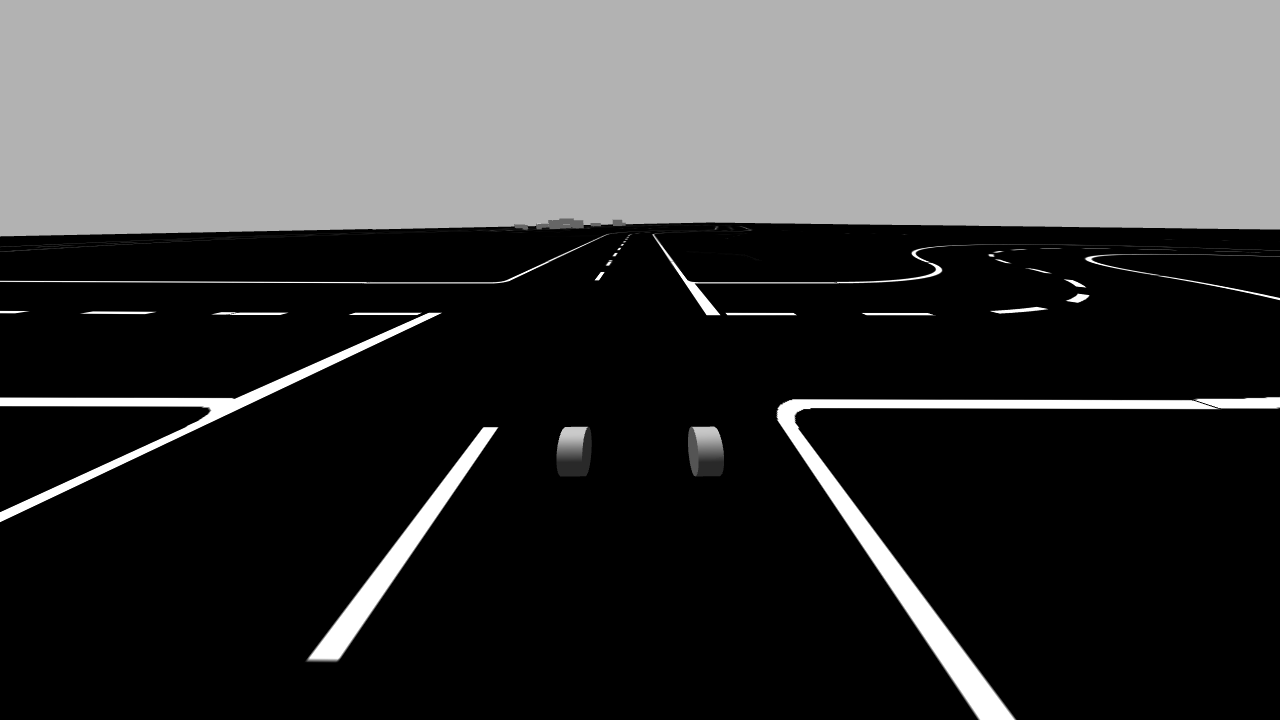
\includegraphics[width=0.3\textwidth]{/home/tb/gazebo_road_generation/02_Arbeit_Latex/008_Kapitel7/Bilder/crossing}% keine extention: w�hlt jpg f�r DVI
  \caption[Kreuzungserkennung]%
           {\label{fig:Kreuzungserkennung}%
           Eine detektierte Kreuzung.}
\end{center}
\end{figure}






\section{Bodenmarkierungs- und Hinderniserkennung}
\label{sec:Bodenmarkierungs- und Hinderniserkennung}

Wird im Bild keine Kreuzung ,Ziellinie und kein Zebrastreifen erkannt, dann wird das Verfahren der Bodenmarkierungs- und Hinderniserkennung ausgef�hrt.
Das Verfahren arbeitet auf dem Graustufenbild in Birdseye-Perspektive.
Der Algorithmus setzt auf die gefundenen Au�enlinienpunkte des Line-Validation-Table-Creators in Fahrtrichtung auf.
Orthogonal zu den Richtungswinkeln der Au�enlinienpunkte wird ein Muster bestehenden aus einem Kreis und einer den Kreis in der Mitte durchlaufenden Linie in beiden Fahrspuren ausgelesen.
F�r das Auslesen der Linie wird die OpenCV-Funktion Lineiterator verwendet.
Das Auslesen des Kreises wird mit der Funktion radialScan realisiert.
Von beiden Au�enlinien aus, kann in beiden Fahrspuren nach Hindernissen und Bodenmarkierungen gesucht werden. Eine definierte Suchweite mit zugeh�riger Schrittweite legt fest, wie weit f�r vor dem Fahrzeug gesucht werden soll.

\begin{figure}[H]
\begin{center}
  \includegraphics[width=0.4\textwidth]{/home/tb/gazebo_road_generation/02_Arbeit_Latex/008_Kapitel7/Bilder/marking_box_search}% keine extention: w�hlt jpg f�r DVI
  \caption[Das Suchmuster der Bodenmarkierung- und Hinderniserkennung]%
           {\label{fig:Das Suchmuster der Bodenmarkierung- und Hinderniserkennung}%
           Das Suchmuster der Bodenmarkierung- und Hinderniserkennung.}
\end{center}
\end{figure}


Wie auch bei der Ziellinien- und Zebrastreifensuche wird nach dem Auftauchen eines bestimmten Segmenten-Musters gesucht.
Um ein Hindernis zu erkennen, muss ein Segment in der Suchlinie gefunden werden, welches �ber einer festgelegten Breite liegt. Dies gilt auch f�r die radiale Suche.
Werden viele kleinere Segmente in der entsprechenden Fahrspur gefunden deutet dies auf eine Bodenmarkierung hin.

\begin{figure}[H]
\begin{center}
  \includegraphics[width=0.4\textwidth]{/home/tb/gazebo_road_generation/02_Arbeit_Latex/008_Kapitel7/Bilder/box}% keine extention: w�hlt jpg f�r DVI
  \caption[Erkennung eines Hindernisses]%
           {\label{fig:Erkennung eines Hindernisses}%
           Eine detektierte Box in der Fahrbahn.}
\end{center}
\end{figure}


\begin{figure}[H]
\begin{center}
  \includegraphics[width=0.4\textwidth]{/home/tb/gazebo_road_generation/02_Arbeit_Latex/008_Kapitel7/Bilder/marking}% keine extention: w�hlt jpg f�r DVI
  \caption[Erkennung einer Bodenmarkierung]%
           {\label{fig:Erkennung einer Bodenmarkierung}%
           Eine detektierte Geschwindigkeitsbegrenzungsmarkierung in der Fahrbahn.}
\end{center}
\end{figure}




%
%% Kapitel: Kapitel 4
%%======================================================================

\chapter{Klassifikation von Geschwindigkeitsbodenmarkierungen}
\label{cha:Klassifikation von Geschwindigkeitsbodenmarkierungen} \index{Klassifikation von Geschwindigkeitsbodenmarkierungen}
%
%


\section{Aufbau des Machine-Learning Frameworks}
\label{sec:Aufbau des Machine-Learning Frameworks}

Bei der Wahl der Programmiersprache fiel die Wahl auf Python. Es ist eine Objektorientierte Programmiersprache die sich vorallem im Wissenschaftlichen Bereich immer mehr beliebtheit erfeut. Vorallem im Datascience und Machine Learning Umfeld findet Python h{\"a}ufig seine Anwendung. Durch seine dynamische Datentypverwaltung und der Strukturierung durch Einr{\"u}cken des Codes ist er sehr {\"u}bersichtlich. Zudem stehen viele Software-Module durch die gro{\ss}e Python-Community zur Verf{\"u}gung was Python zu einem sehr m{\"a}chtigen Werzeug macht.
F{\"u}r das integrieren der Module zu einem gesamtsystem wurde die Anaconda Python/R Data Science Platform genutzt. Sie beihnalten den Conda Paketmanager welcher eine gro{\ss}e Unterst{\"u}tzung beim finden und installieren von Softwarepaketen ist. Auch werden abh{\"a}ngigkeiten von verschiedenen Softwareversion der Module automatisch durch Conda gel{\"o}st was sonst oft zu Problemen gef{\"u}hrt hat. Conda ist auch ein Umgebungsmanager mit dem Software lokal abgetrennt in einer eigenen Umgebung programmiert werden kann. Dies ist n{\"u}tzlich wenn etwa Verschiedene Python Versionen auf dem selben System genutzt werden m{\"u}ssen.
Im Folgenden sind die Python-Module aufgelistet die in der Arbeit ihre Verwendung fanden.

\begin{enumerate}

\item[] \textbf{Pycharm}\hfill \\
Pycharm ist eine integrierte Entwicklungsumgebung f{\"u}r Python. 
Sie assisitiert beim Programmieren durch, Codevervollst{\"a}ndigung sowie syntax und Fehler Hervorhebung. Der Hauptgrund f{\"u}r die Wahl dieser IDE war der effizeinte Python-Debugger durch den man auch beim Arbeiten auf gro{\ss}en Datenstrukturen einen leichten {\"U}berblick {\"u}ber das Verhalten des Codes bekommt.


\item[] \textbf{Numpy}\hfill \\
Die Programmbibliothek Numpy steht f{\"u}r Numeric Python. Sie bietet funktionen zum arbeiten mit gro{\ss}en Arrays und Matrizen. Auch numerische Berechnungen und mathematische Routinen sind implementiert. Da viele Numpy-Operationen in C implementiert sind hat die Bibliothek auch eine gute Performance.


\item[] \textbf{Matplotlib}\hfill \\
Durch Matplotlib lassen sich Mathematische zusammenh{\"a}nge oder Daten visualisieren. 
Mit nur wenigen Codezeilen lassen sich zum Beispiel Histogramme, Balkendiagramme, Korrelationsdiagramme oder Punktwolken visualisieren. Die Bibliothek ist eine kostenfreie alternative zur visualisierung mit Matlab.


\item[] \textbf{Pandas}\hfill \\
Pandas ist eine Python-Paket welches zur Datenanalyse und verarbeitung von Daten genutzt wird.
Vorallem die DataFrames eine zweidimensionale Datenstruktur welche Spalten mit verschiedenen Datentypen beinhalten kann sind sehr n{\"u}tzlich zur vorverarbeitung von Datens{\"a}tzen f{\"u}r das maschinelle lernen. Eine Speicherstelle kann einfach {\"u}ber ihren Spaltenname und den Zeilenindex angepsrochen werden. Es lassen sich schnell Statistiken {\"u}ber einzelne oder mehrer Spalten berechnen oder einzelne Ausrei{\ss}er lokalisieren. Auch das lesen und speichern von zum Beispiel CSV, Text-Dateien oder SQL-Datenbanken ist gegeben.

\item[] \textbf{Scikit-learn}\hfill \\
Scikit-Learn ist eine Software-Bibliothek zum maschinellen Lernen f{\"u}r Python.
Sie bietet verschiedene Klassen von Algorithmen an. Diese sind Regressions-, Klassifikations sowie Clusteralgorithmen. Es werden auch Funktionen zur Aufbereitung von 
Datens{\"a}tzen angeboten da manche Verfahren andere Representationen von Trainingsdaten ben{\"o}tigen um effizient lernen zu k{\"o}nnen. Weiter bieten Scikit-Learn Metriken zur Bewertung von trainierten Modellen. Viele Kernfunktionen sind in Cython geschrieben um die Dauer des Trainings zu beschleunigen. Eine beschleunigung durch GPUs ist nicht implementiert. Alle Berechnungen finden auf dem Hauptprozessor statt.

\item[] \textbf{Tensorflow}\hfill \\
Tensorflow ist ein Framework f{\"u}r das maschinelle Lernen entwickelt von Google.
Es wird vorallem zum Training von Deep-Learning Architekuren verwendet.
Rechenschritte werden als Datenflussgraphen dargestellt um Abh{\"a}ngigkeiten zwischen einzelnen Operationen zu representieren.
Durch die NVIDIA-CUDA Erweiterung von Tensorflow k{\"o}nnen Berechnungen durch GPUs hoch parallelisiert werden und mit der zus{\"a}tzlichen Programmierbibliothek NVIDIA-cuDNN wird es
erm{\"o}glicht auch K{\"u}nstliche Neuronale Netze GPU-beschleunigt zu optimieren.
\item[] \textbf{Keras}\hfill \\
Keras ist eine Deep-Learning Bibliothek und High-Level API. Es ist die Schnittstelle f{\"u}r verschiedene Backends wie Tensorflow oder Theano. Die API hat eine hohe Bedienerfreundlichkeit nd erm{\"o}glicht ein schnelles und einfaches Prototyping von neuronalen Netzen.
\item[] \textbf{Jupyter-Notebook}\hfill \\
Jupyter-Notebook ist eine Webapplikation die es erlaubt den Code und dessen Dokumentation in einer geteilten Umgebung zu verwenden. Es wird gerne in Datascience Projekten genutzt. Sehr n{\"u}tzlich sind sie falls man sich noch in der Protoypenphase befindet. Code wird in verschiedenen Zellen aufgef{\"u}hrt dies erlaubt es einen bestimmten Code-Block auszuf{\"u}hren ohne das Gesamte Programm neuzustarten.  Dadurch m{\"u}ssen Daten nicht immer wieder erneut in den RAM geladen werden oder es k{\"o}nnen Parameter beim Training von ML-Modellen flexibel angepasst werden. Auch bei der Visualisierung von Daten ist es hilfreich.



\end{enumerate}


\section{Klassifikation durch Template Matching}
\label{sec:Klassifikation durch Template Matching}

Da die Geschwindigkeitsmarkierungen auf der Fahrbahn immer gleich aussehen wurde sich dazu entschieden, die Markierungen {\"u}ber ein Template-Matching zu klassifizieren.
Daf{\"u}r wird die OpenCV-Funktion MatchTemplate verwendet.
Die Bilder f{\"u}r das Template-Matching wurden aus der Simulation heraus extrahiert und extern abgespeichert. Zur Laufzeit des Programms werden die Templates in das Programm eingeladen.

\begin{figure}[H]
\begin{center}
  \includegraphics[width=0.8\textwidth]{/home/tb/gazebo_road_generation/02_Arbeit_Latex/009_Kapitel8/Bilder/roadspeedsigngs}% keine extention: wählt jpg für DVI
  \caption[Geschwindigkeitsmarkierungstemplates]%
           {\label{fig:Geschwindigkeitsmarkierungstemplates}%
           Geschwindigkeitsmarkierungstemplates.
           }
\end{center}
\end{figure}

Die Templates haben eine Dimension von XXX welche genau derselben Gr{\"o}{\ss}e der Geschwindigkeitsmarkierungen in der Simulation in Birdseye-Perspektive entsprechen. Das Bild auf dem TemplateMatch angewandt wird, wird aus der Topic /road\_sign ausgelesen.
Die Funktion MatchTemplate faltet das Template {\"u}ber den Bildbereich und berechnet einen Score abh{\"a}ngig von der ausgew{\"a}hlten Methode. Folgende Methoden wurden getestet.

\begin{enumerate}

\item[] \textbf{CV\_TM\_SQDIFF}\hfill \\
Berechnet die euklidische Distanz nach folgender Formel:

\begin{figure}[H]
\begin{center}
  \includegraphics[width=0.8\textwidth]{/home/tb/gazebo_road_generation/02_Arbeit_Latex/009_Kapitel8/Bilder/sqdiff}% keine extention: wählt jpg für DVI
  \caption[SQDIFF]%
           {\label{fig:SQDIFF}%
           Berechnung der euklidischen Distanz zwischen Pixel und Template.
           }
\end{center}
\end{figure}




\item[] \textbf{CV\_TM\_CCORR}\hfill \\
Berechnet die Korrelation nach folgender Formel:

\begin{figure}[H]
\begin{center}
  \includegraphics[width=0.8\textwidth]{/home/tb/gazebo_road_generation/02_Arbeit_Latex/009_Kapitel8/Bilder/ccorr}% keine extention: wählt jpg für DVI
  \caption[CCORR]%
           {\label{fig:CCORR}%
           Berechnung der korrelation zwischen Pixel und Template.
           }
\end{center}
\end{figure}


\end{enumerate}


$$R(x,y) = \sum_{x',y'} (T(x',y')-I(x+x',y+y'))^2$$  

$$R(x,y) = \sum_{x',y'} (T(x',y') \cdot I(x+x',y+y'))$$  


Die Ausgabe von MatchTemplate ist eine OpenCV-Matrix mit den Werten der Aktivierungen durch das Falten mit dem entsprechenden Template.
Bei der Methode CV\_TM\_SQDIFF gibt der minimale Wert in der Matrix den besten Score an. Bei der Methode CV\_TM\_CORR gibt der maximale Wert den besten Score an. Diese werden mit der OpenCV-Funktion minMaxLoc ermittelt.
Alle neun Scores der Templates werden mit dem Bild aus /road\_sign berechnet.
Das Template mit dem besten Score steht f{\"u}r die klassifizierte Geschwindigkeitsmarkierung. 



\section{Aufbereitung des MNIST-Trainingsdatensatzes}
\label{sec:Aufbereitung des MNIST-Trainingsdatensatzes}

F{\"u}r das training der Machine-Learning Modelle zur Klassfikation der Geschwindigkeitsbodenmarkierungen wurde der MNIST-Datensatz verwendet.
Dieser Besteht aus einem Trainingsdatensatz mit 54077 Handgeschriebenen einstelligen Ziffern von null bis neun mit einer Dimension von 28x28. Und einem zugeh{\"o}rigen Testdatensatz mit 9020 Ziffern.
Da die Geschwindigkeitsmarkierungen beim Carolo-Cup nur zweistellige Zahlen beeinhalten wurden die nullen aus dem Datensatz zuf{\"a}llig an die Zahlen eins bis neun angeh{\"a}ngt. Dadurch ergibt sich eine Bilddimension von 28x56 mit dem die verschiedenen Machine-Learning Modelle trainiert wurden.

\begin{figure}[H]
\begin{center}
  \includegraphics[width=1.0\textwidth]{/home/tb/gazebo_road_generation/02_Arbeit_Latex/009_Kapitel8/Bilder/mnist}% keine extention: wählt jpg für DVI
  \caption[Aufbereitete Features des MNIST-Datensatzes]%
           {\label{fig:Aufbereitete Features des MNIST-Datensatzes}%
           Aufbereitete Features des MNIST-Datensatzes.
           }
\end{center}
\end{figure}

\section{Klassifikation durch Random Forest}
\label{sec:Klassifikation durch Random Forest}

Random Forest ist ein {\"u}berwacht trainiertes maschinelles Lernverfahren welches aus einem Ensemble von randomisiert trainierten Entscheidungsb{\"a}umen besteht. Entwickelt wurde das Verfahren 2001 durch Leo Breiman. Es ist m{\"o}glich den Algorithmus als Klassifikiationsansatz oder als Regressionsansatz zu implementieren. Bei der Auswertung von Random Forest wird die Entscheidung nach einem Mehrheitsvotum durch die einzelnen Entscheidungsb{\"a}ume getroffen.
Random Forest ist eines der am h{\"a}ufigsten genutzten Algorithmen zur Auswertung von Daten. Es liefert sehr gute Ergebninsse auf verschiedenste Datens{\"a}tze und hat eine geringe Trainingszeit im vergleich zu neuronalen Netzen. Das Verfahren kann mit tausenden von Eingangsvariablen umgehen und es sind bin{\"a}re kategoriale als auch numerische Merkmals-Typen lernbar.
Zudem ist das Verfahren robust gegen {\"U}beranpassung durch das training der einzelnen B{\"a}ume mit Boostrap-Stichprobieren und des Mehrheitsvotums bei der Entscheidungsf{\"a}llung. 
Random Forest kommt auch mit outliern und unstandardisierten Daten zurrecht.
Auch ist es m{\"o}gliche ein Einsehen in das trainierte Modell zu bekommen. Dadurch kann die prozentuale wichtigkeit einzelner Trainingsmerkmale bei der Entscheidungsfinding erhalten werden.

\subsection{Aufbau eines Entscheidungsbaums}
\label{subsec:Aufbau eines Entscheidungsbaums}

Ein Entscheidungsbaum wird umgekehrt mit seiner Wurzel an der Spitze dargestellt.
Sie sind aus einer Kombinaition von vier Komponenten aufgebaut.


\begin{enumerate}

\item[] \textbf{Wurzelknoten}\hfill \\
Stellt den Input des Baumes dar und f{\"a}llt die erste Entscheidung zur Separation der Eingangsdaten.

\item[] \textbf{Innere Knoten}\hfill \\
Beeinhalten logische Tests welche durch ein {\"u}berwachtes Training spezifiziert wurden


\item[] \textbf{Bl{\"a}tter}\hfill \\
Sie sind das Ende des Baumes und stehen f{\"u}r das Ergebnis der Klassifikation.

\item[] \textbf{Kanten}\hfill \\
Verbindung zwischen Wurzelknoten, Innerer Knoten und Bl{\"a}ttern
\end{enumerate}


Vom Wurzelknoten aus wird der Merkmalsvektor einer Oberservation durch den Baum gef{\"u}hrt bis er an einem Blatt angelangt ist. Dadurch wird die Oberservation klassifiziert.
Der Weg der {\"u}er die Kanten und inneren Knoten durchlaufen wird ist abh{\"a}ngig von den logischen Tests.



\begin{figure}[H]
\begin{center}
  \includegraphics[width=0.5\textwidth]{/home/tb/gazebo_road_generation/02_Arbeit_Latex/009_Kapitel8/Bilder/tree}% keine extention: wählt jpg für DVI
  \caption[Aufbau eines Entscheidungsbaums]%
           {\label{fig:Aufbau eines Entscheidungsbaums}%
           Aufbau eines Entscheidungsbaums.
           }
\end{center}
\end{figure}

\subsection{Training von Random-Forest durch den CART-Algorithmus}
\label{subsec:Training von Random-Forest durch den CART-Algorithmus}

Der CART-Algorithmus (Classification and Regression Tree) ist ein Verfahren um die logischen Tests der Knoten zur korrekten Klassifikation zu lernen. Die Modellstruktor des Entscheidungsbaumes ist dabei nicht von vorneherin festgelegt sondern wird durch die Daten bestimmt. 
Beim training des Algorithmus werden N Samples von Observationen mit Merkmals-Vektoren und bekannten Labeln zuf{\"a}llig aus dem gesamten Datensatz mit der selben gr{\"o}{\ss}e N  ausgew{\"a}hlt. Bei der Auswahl kann auch die selbe Observation mehrmals gezogen werden. Dies Wird  Bootstrapping genannt. 
F{\"u}r jeden Entscheidungsbaum des Random Forest Algorithmus wird ein zuf{\"a}lliges Subset von Merkmalen ausgew{\"a}hlt. Bei M Input-Merkmalen also m<M Merkmale die f{\"u}r jeden einzelnen Entscheidungsbaum konstant gehalten werden. Bei der Klassifikation wird meist die Wurzel aus der Anzahl der gesamten Merkmale genommen m = sqrt(M) [vgl. Hastie et al., S. 592 [16]]. Dies ist ein weiterer Trick um dem Algorithmus eine bessere Generalisierung zu verschaffen da dadurch die Entscheidungsb{\"a}ume weniger miteinander korrelieren.
Der CART-Algorithmus in jedem Schritt anhand eines der zuf{\"a}llig ausgew{\"a}hlten Merkmale durch einen logischen Test das Set in zwei getrennte Gruppen aufzuteilen (bin{\"a}rer Split).

Um das Merkmal zu finden welches die Daten am besten teilt wird das Gini-Unreinheitsma{\ss} verwendet. Es gibt an wie Wahrscheinlich es ist einen Datenpunkt falsch zu klassifizieren.
Hat man J verschiedene Klassen ist  p(i) die Wahrscheinlichkeit einen Datenpunkt der Klasse i zu w{\"a}hlen. Somit Berechnet sich das Gini-Unreinheitsma{\ss} nach folgender Formel:

\begin{figure}[H]
\begin{center}
  \includegraphics[width=1.0\textwidth]{/home/tb/gazebo_road_generation/02_Arbeit_Latex/009_Kapitel8/Bilder/gini}% keine extention: wählt jpg für DVI
  \caption[Formel zur Berechnung des Gini-Unreinheitsmass]%
           {\label{fig:Formel zur Berechnung des Gini-Unreinheitsmass}%
           Formel zur Berechnung des Gini-Unreinheitsmass.
           }
\end{center}
\end{figure}
  
$$ I_{G}(p)  = \sum_{i=1}^{J} p_{i} \sum_{k \neq i} p_{k} = \sum_{i=1}^{J} p_{i}(1-p_{i}) = \sum_{i=1}^{J} (p_{i} - p_{i}^2) = \sum_{i=1}^{J} p_{i} - \sum_{i=1}^{J} p_{i}^2 = 1 - \sum_{i=1}^{J} p_{i}^2 $$

Die Berechnung eines Splits wird folgend an einem Beispiel veranschaulicht.
Angenommen man habe drei verschiedene Klassen mit insgesamt 80 Observationen welche Merkmale und zugeh{\"o}rige Klassen in sich vereinen.
Davon befinden sich 19 Observationen in der Klasse eins, 21 Observationen in der Klasse zwei und 40 Observationen in der Klasse drei. Das Gini-Unreinheitsma{\ss) berechnet sich nun zu:


${ \displaystyle 1- [ (\frac{19}{80})^2 + (\frac{21}{80})^2 + (\frac{40}{80})^2] = 0,6247 }$


Um den logischen Test f{\"u}r den besten bin{\"a}ren Split {\"u}ber ein Merkmal der Observationen zu finden werden die Gini-Unreinheitsma{\ss)e f{\"u}r alle m{\"o}glichen Werte durchgetestet.
Angenommen man w{\"u}rde das Merkmal X1 bei X1 > 2 aufteilen und die Observationen w{\"u}rden sich nach Klassen folgederma{\ss)en aufteilen:

Linke Kante: 16, 9, 0\\
Rechte Kante : 3, 12, 40

Dann errechnet sich das Gini-Unreinheitsma{\ss} zu:

Linke Kante:   ${ \displaystyle 1 - [ (\frac{16}{25})^2 + (\frac{9}{25})^2] = 0,4608}$\\
Rechte Kante: ${ \displaystyle 1 - [ (\frac{3}{55})^2 + (\frac{12}{55})^2+ (\frac{40}{55})^2] = 0,4205}$

Um die Qualit{\"a}t des Splits zu beurteilen werden die Unreinheitsma{\ss)e je Kante mit der Anzahl in Sie hinfeinfallender Observationen Gewichtet und die Werte gemittelt. 
Dies ergibt das mittlere Gewichtete Unreinheitsma{\ss) f{\"u}r den Split X1 > 2.

${ \displaystyle \frac{25}{80} * Gini Linke Kante + \frac{55}{80} * Gini Rechte Kante = 0,4331}$

Der Gewinn des Splits kann nun berechnet werden indem das Gini-Unreinheitsma{\ss) nach dem Split von dem Gini-Unreinheitsma{\ss) vor dem Split subtrahiert wird. Dieser Wert wird auch Gini-Gain genannt. 

$ {\displaystyle 0,6247 - 0,4331 = 0,1916}$

Der Split der die Observationen mit dem gr{\"o}{\ss)ten Gewinn aufteilt wird anschlie{\ss)end im Entscheidungsbaum verwendet und es findet ein neuer Split f{\"u}r jede Kante statt.
Dies wird wiederholt bis ein festgelegtes Stoppkriterium erreicht ist oder in eine Kante nurnoch eine Observation f{\"a}llt. Alle Knoten die nichtmehr gesplittet werden, werden zu Bl{\"a}ttern.
Ein Blatt steht am Ende des durch Trainings gewachsenen Baumes f{\"u}r jene Klasse welche am h{\"a}ufigsten in sie hineinf{\"a}llt.

\begin{figure}[H]
\begin{center}
  \includegraphics[width=1.0\textwidth]{/home/tb/gazebo_road_generation/02_Arbeit_Latex/009_Kapitel8/Bilder/rfm}% keine extention: wählt jpg für DVI
  \caption[Ein Random Forest Modell]%
           {\label{fig:Ein Random Forest Modell}%
           Ein Random Forest Modell.
           }
\end{center}
\end{figure}

\subsection{Auswertung von Random-Forest}
\label{subsec:Auswertung von Random-Forest}


F\"ur das Training und die Auswertung des Random Forest Models wurden die Bildsamples von der Dimension 28x56 in die Dimension 1x1568 umtransformiert.
Das Training dauerte ungef{\"a}hr zehn Sekunden.
Die Auswertung auf den Testdatensatz ergab eine Genauigkeit von 94,1\%.
Da die Bewertung über die Genauigkeit bei einem multinomialen Klassifikatior nicht genügt ist in folgender Abbildung die Auswertung auf den Testdatensatz über eine Verwirrungsmatrix gegeben.

\begin{center}


\begin{tabular}{|c|c|c|c|c|c|c|c|c|c|}
\hline
    & \textbf{10} & \textbf{20} & \textbf{30} & \textbf{40} & \textbf{50} & \textbf{60} & \textbf{70} & \textbf{80} & \textbf{90} \\
\hline
\textbf{10} & 1117 &  3 &  2 &  1 &  1 &  2 &  0 &  9 &  0 \\
\hline
\textbf{20} &  5  & 989 &   8 &   3 &   3 &   2 &   6 &  15 &   1 \\
\hline
\textbf{30} & 0  & 21 & 935  &  0 &  19 &   1 &   8 &  21 &   5 \\
\hline 
\textbf{40} &  2 &   7 &   2 & 924  &  3  &  2 &   4  &  5 &  33 \\
\hline 
\textbf{50} &  3 &   6 &  38 &   9 & 816 &  10 &   1 &   8 &   1 \\
\hline 
\textbf{60} &  4  &  2 &   0 &   6 &  12 & 928 &   0  &  5 &   1 \\
\hline 
\textbf{70} &  9  & 20 &   9 &   7 &   0  &  1 & 965  &  7 &  10 \\
\hline 
\textbf{80} &  2  &  6 &  19 &  15 &  17 &   9  &  3 & 894  &  9 \\
\hline
\textbf{90} &  8  &  4 &  23 &  30 &   7 &   1 &  11 &   9 & 916 \\
\hline
\end{tabular}

\end{center}


\section{Klassifikation durch Convolutional Neural Networks}
\label{sec:Klassifikation durch Convolutional Neural Networks}

Ein CNN ist eine Art Künstliches Neuronales Netz. Sie sind sehr gut da-
für geeignet Bilder zu klassifizieren. Inspiriert wurden CNNs durch den visuellen Kortex Gehirns. Dieser besitzt Zell-Regionen die auf unterschiedliche Bereiche des Blickfelds reagie-
ren. Durch das einsetzen einer Mikroelektrode in den prim\"aren visuellen Kortex einer Katze,
konnten Hubel und Wiesel 1961 beweisen, dass einzelne neuronale Zellen im Gehirn nur auf die
Pr\"asenz von Linien und Kanten in spezieller Orientierung reagieren [31]. Manche reagierten
zum Beispiel nur auf horizontale, andere auf vertikale Linen oder Kanten. Au{\ss}erdem fanden sie
heraus, dass diese Nervenzellen in einer S\"aulen-Architektur aufgebaut sind. Untersuchungen
deuteten darauf hin, dass diese Informationsverarbeitung in den höheren Schichten fortgef\"uhrt
wird, so dass Nervenzellen auf komplexe Formen wie etwa Buchstaben und Gesichter reagie-
ren. CNNs ahmen diese Struktur im mathematischen Sinne nach. Sie versuchen bestimmte
Charakteristiken, von einem Objekt in einem Bild, durch Faltungen mit speziellen Filtern zu
extrahieren und daraus die Objektklasse abzuleiten. Sie sind aus verschiedene Lagen aufge-
baut. Um eine CNN-Architektur zu erschaffen, wird eine Kombination aus drei Hauptlagen
verwendet, dies sind das Convolutional Layer, das Pooling Layer und das Fully-Connected
Layer. Für tiefere Informationen zu CNN verweise ich auf meine Bachelorarbeit.


\subsection{Aufbau und Training der CNN Architektur}
\label{subsec:Aufbau und Training der CNN Architektur}

Das CNN-Model wurde durch Keras mit dem Tensorflow als Backend implementiert und trainiert. Das Model besitzt im Eingangslayer eine Convolutional-Layer mit 32 Kernel der Gr\"o{\ss}e  3x3 und der Rectified Linear Unit als Aktivierungsfunktion. Es nimmt ein Eingangsbild der Dimension 28x56 entgegen welche der Gr\"o{\ss}e der vorverarbeiteten MNIST-Daten entspricht.
Es folgt ein weiteres Convolutional-Layer mit 64 Kernel der Gr\"o{\ss}e 3x3 wieder gefolgt von der gleichen Aktivierungsfunktion. Es folgt ein Max-Pooling-Layer mit einem Kernel der Dimension 2x2. Darauf schlie{\ss}t sich ein Dropout-Layer mit 75\% Haltungsrate an um bessere Generalisierung auf nicht gesehene Daten zu erm\"oglichen.
Das n\"achste Layer ist ein Feed-Forward-Layer mit 128 Neuronen mit anschlie{\ss}ender Relu-Aktivierungsfunktion. Es folgt wieder ein Dropout-Layer mit einer Haltungsrate von 50\%. Das letzte Layer ist das Ausgangs-Layer mit einer Softmax-Aktivierungsfunktion.
Als Optimierungsalgorithmus wurde Adadelta verwendet. Trainiert wurde das Netz über 12 Epochen mit einer Batch-Size von 128.


\subsection{Auswertung der trainierten CNN-Architektur}
\label{subsec:Auswertung der trainierten CNN-Architektur}

Das Training des CNNs dauerte ungef\"ahr f\"unf Minuten auf einer Nvidia Titan X Grafikkarte. Bei der Auswertung auf den Testdatensatz ergab sich eine Genauigkeit von 98,4\%. Im folgenden ist die Verwirrungsmatrix für die Auswertung auf den Testdatensatz gegeben.


\begin{center}


\begin{tabular}{|c|c|c|c|c|c|c|c|c|c|}
\hline
    & \textbf{10} & \textbf{20} & \textbf{30} & \textbf{40} & \textbf{50} & \textbf{60} & \textbf{70} & \textbf{80} & \textbf{90} \\
\hline
\textbf{10} & 1124 &  1 &  3 &    0 &   1 &    4 &    0 &  2 &    0  \\
\hline
\textbf{20} &  6 & 1007 &  1 &    3 &    0 &    2 &    9 &  4 &  0 \\
\hline
\textbf{30} & 0&    1&  998&    0&    3&    0&    2&    5&    1 \\
\hline 
\textbf{40} &  0&    0&    0&  968&    0&    5&    0&    2&    7 \\
\hline 
\textbf{50} &  1&    0&    7&    0&  878&    3&    0&    2 &    1 \\
\hline 
\textbf{60} &  2&    0&    1&    2&    3&  948&    0&    2&    0 \\
\hline 
\textbf{70} &  3&    4&    0&    0&    0&    0& 1018&    1&    2 \\
\hline 
\textbf{80} &  0&    0&    2&    3&    3&    4&    3&  955 &  4 \\
\hline
\textbf{90} & 5&    0&    2&    8&    4&    0&   7&   3& 980 \\
\hline
\end{tabular}

\end{center}





%%
%% Kapitel: Kapitel 4
%%======================================================================

\chapter{Aufbau eines Testframeworks mit Google-Test}
\label{cha:Aufbau eines Testframeworks mit Google-Test} 
\index{Aufbau eines Testframeworks mit Google-Test}
%
%

Google-Test ist eine Unit-Test-Bibliothek f\"ur die Programmiersprache C++, die auf der xUnit-Architektur basiert. Das xUnit Framework erlaubt das \"Uberpr\"ufen verschiedener Elemente von Software, wie etwa Funktionen und Klassen. Um eine fehlerfreie Software zu gew\"ahrleisten ist ein Unit-Testing der verschiedenen Softwaremodule unumg\"anglich.
Aus diesem Grund wurde die gesamte Bildverarbeitungssoftware modular gestaltet. Jede Funktion der verschiedenen Klassen besitzt definierte Ein- und Ausgangsvariablen und ist intern von keinen weiteren Variablen abh\"angig um die Funktionen separiert testen zu k\"onnen.
F\"ur jede Klasse der in XXX beschriebenen Bildverarbeitungsalgorithmen wurde ein angepasstes Unit-Test-Modul geschrieben welches getrennt von der Hauptsoftware ausf\"uhrbar ist. Es erlaubt die Initialisierungsparameter anzupassen und die Funktionen mit Mock-Objekten testen zu lassen. Auch k\"onnen die ganzen Klassen auf ihr Verhalten auf Einzelbilder getestet werden. Das Testen wird auch durch eine visualisierte Ausgabe der Verarbeitung des Eingangsbildes erm\"oglicht.











%%
%% Kapitel: Kapitel 4
%%======================================================================

\chapter{Ergebnisse}
\label{cha:Ergebnisse} \index{Mittelliniensuche und Grapherzeugung}
%
%




\section{Vanishing-Point-Search-Algorithmus}
\label{section:Vanishing-Point-Search-Algorithmus} 

Findet der Vanishing-Point Algorithmus Schnittpunkte zwischen linken und rechten Fahrbahnlinien welche auch im korrekten Abstand zum Fahrzeug liegen ist dies ein robuster Indikator nach dem gefahren werden kann.
Durch einen gefundenen Vanishing-Point kann zugleich auch der einzuschlagende Lenkwinkel zwischen Fahrzeugmittelpunkt und Vanishing-Point berechnet werden was ein weiterer Vorteil des Verfahrens ist.
Auch bei einer fehlenden Au{\ss}enlinie kann nach einer erkannten Hough-Linie gefahren werden.
Umso kleiner der Bereich in dem nach Hough-Linien gesucht wird ist desto sicherer sind die Ergebnisse des Verfahrens. Es kann aber passieren das wenn sich das Fahrzeug nicht genau in der Mitte einer Fahrspur befindet keine entsprechenden Hough-Linien gefunden werden und somit das Verfahren und Ergebnis terminiert. Da die Kantenextraktion und die Hough-Linien-Suche nur auf einem kleinen Bildbereich vor dem Fahrzeug ausgef{\"u}hrt werden liefert der Algorithmus eine sehr gute Performance und ist nicht Rechenintensiv. Dies erlaubt es Ihn auch auf einem kleinen Mikrocontroller auszuf{\"u}hren. Zudem sind der Canny-Edge- und der Hough-Lines-Algorithmus durch anpassen der OpenCV-Funktion leicht parallelisierbar und k{\"o}nnen dadurch noch schneller ausgef{\"u}hrt werden.  



\section{Start-of-Lines-Search-Algorithmus}
\label{section:Start-of-Lines-Search-Algorithmus} 
Wird das eindeutige Fahrbahnmuster durch Start-of-Line-Search erkannt ist dies ein sicheres Merkmal f{\"u}r eine korrekte Orientierung des Fahrzeugs in der Fahrbahn. Die Startparameter von Start-of-Lines-Search werden denen von Vansishing-Point-Search vorgezogen da sie f{\"u}r eine einduetigere Charakteristik stehen. Auch dieses Verfahren ist wenig Recheninstensiv und f{\"u}r einen kleinen Mikrocontroller geeignet.
Jedoch findet der algorithmus nur dann das entsprechende Muster wenn alle Fahrbahnlinien vorhanden sind und die Mittellinie sich im Suchebereich befindet ansonsten terminiert das Verfahren ohne Ergebnis.
Auch bei Start-of-Lines-Search bestimmt die Gr\"o{\ss}e der Liniensuchbereiche die Genauigkeit des Algorithmus. Da das Verfahren Linien auf ihre korrekte Breite untersucht liefert es eine zus\"atzliche Sicherheitsstufe. Falls sich aber ein Objekt neben der Fahrspur befindet wie zum Beispiel eine Box welche die Linie {\"u}berdeckt stimmt die Segmentbreite nicht {\"u}berein und das Verfahren terminiert ohne gefundenes Muster.


\section{Line-Follower-Algorithmus}
\label{section:Line-Follower-Algorithmus}
Der Line-Follower Algorithmus ist abh\"angig von den Startparametern von Start-of-Lines-Search oder Vanishing-Point-Search. Somit werden nur gute Ergebnisse geliefert wenn auch die Startparameter korrekt sind.
Das Verfahren kann die Au{\ss}enlinien sehr weit Verfolgen. Da das Verfahren rekursiv ausgef\"uhrt wird ist die genaue Laufzeit nicht bestimmbar denn sie ist abh\"angig von den festgelegten Terminierungskriterien. Au{\ss}erdem kann es passieren das der Algorithmus an einer Positionen stecken bleibt oder wie es bei Boxen vorkommen kann sich zuf\"allig in verschiedene Richtungen bewegt.
Ein Vorteil ist das sich durch die Linienabsuche zus\"atzlich die Richtungswinkel vermerken lassen und somit eine Kreuzung leicht detektiert werden kann. Bei auftauchen einer Ziellinie kann das Verfahren aber auch eine Falsche Suchrichtung einschlagen we{\ss}wegen die Ergebnisse von Line-Follower weiter evaluiert werden m\"ussen.
 

\section{Line-Points-Reduce-Algorithmus}
\label{section:Line-Points-Reduce-Algorithmus}

Der Ramer-Douglas-Peucker-Algorithmus reduziert die Linien-Punkte des Line-Follower-Algorithmus auf markante Punkte welche die Fahrbahnlinien beschreiben. Auch er ist ein rekursiver Algorithmus wodurch die Laufzeit nicht vorhergesagt werden kann. Der Algorithmus erm\"oglicht es die wichtigen Punkte von Line-Follower zu extrahieren und somit den Speicherplatzbedarf im RAM zu reduzieren. Seine Ergebnisse sind abh\"angig von der Qualit\"at der gefundenen Punkte des Line-Follower-Algorithmus. 

\section{Mid-Line-Search-Algorithmus}
\label{section:Mid-Line-Search-Algorithmus}
Die Mittelliniensuche sucht im gesamten Eingangsbild nach Pixeln welche zu Mittellinienstreifen geh\"oren. Anschlie{\ss}end werden Mittellinien-Segmente welche benachbart sind zusammengef\"uhrt. Das Verfahren entdeckt auch Mittellinien welche weit vom Fahrzeug entfernt liegen. Somit ist es auch m\"oglich Kreuzugen durch die Orientierung von gefundenen Mittelliniensegmenten zu detektieren. Au{\ss}erdem k\"onnen \"uber eine Kreuzung hinaus Mittelliniensegmente gefunden werden. Das Verfahren ist sehr rechenintensiv da jedes Pixel des Eingangsbilds einzeln betrachtet wird. Durch die Gruppierung der Mittellinien zu zusammengeh\"origen Segmenten l\"asst sich desweiteren der Winkel an der entsprechenden Fahrbahnposition ermitteln.

\section{Line-Validation-Table-Creation-Algorithmus}
\label{section:Line-Validation-Table-Creation-Algorithmus}

Das Verfahren bewertet die gefundene Au{\ss}en- und Mittelliniensegmente indem es \"uberpr\"uft ob Nachbarliniensegmente vorhanden sind und weist diesen einen Priorit{\"a}ten-Score zu. Dies soll als zus\"atzliche Sicherheitsstufe dienen um robuste Punkte zu finden nach denen gefahren werden kann. Da f{\"u}r die Suche die minimale euklidische Distanz im Vector-Container der Nachbarlinien gesucht wird ist der Algorithmus rechenintensiv jedoch liefert er dadurch sehr sichere Punkte und Bereiche welche das Fahrzeug anschlie{\ss}end befahren kann.  

\section{Rect-Safety-Algorithmus}
\label{section:Rect-Safety-Algorithmus}

Der Algorithmus Wertet die aus Line-Validation-Table-Creation erzeugten Bewertungstabellen in aufeinanderfolgenden Fahrbahnbereichen aus. Dadurch ist es m{\"o}glich Sicherheitskritische Bereich fr{\"u}hzeitig zu erkennen und entsprechend zu agieren. Der Ansatz erm{\"o}glich es auch {\"u}ber Kreuzungen hinaus nach Fahrpunkten zu suchen. Da das Verfahren rekursiv aufgerufen wird bis der Mittelpunkt eines Sicherheitsbereichs nicht mehr im Eingangsbild liegt kann die Laufzeit variieren. Zudem wird die Sicherheitsvorhersage je weiter der Sicherheitsbereich entfernt ist abnehmend vager und sollte weiter validiert werden.

\section{Startboxschrankenerkennung}
\label{section:Startboxschrankenerkennung}
Die Startboxschrankenerkennung detektiert eindeutig den Qr-Code der Startboxschranke. Das Verfahren ist recheninstiv kann jedoch nach dem {\"O}ffnen der Schranke einfach abgeschalten werden.


\section{Zebrastreifen- und Ziellinienerkennung}
\label{section:Zebrastreifen- und Ziellinienerkennung}
Die Zebrastreifen- und Ziellinienerkennungs-Verfahren suchen beide nach einem eindeutigen Muster definiert durch die Segmentbreite von schwarzen und wei{\ss}en Pixelsegmenten. Zudem wird die Anzahl an auftauchenden schwarzen und wei{\ss}en Pixelsegmenten in betracht gezogen, dadurch lassen sich die beiden Markierungen sehr gut unterscheiden.
Durch die definition eines Sichtfelds in welchem die Ziellinie gesucht wird kann die Ziellinie auch in einer Kurve erkannt werden.
Da bei einer Suche nach diesen Bodenmarkierungen fehlklassifikationen auftreten k{\"o}nnen wenn die Suche zu weit vorausschauend initialisiert ist sollte nicht zu weit vor dem Fahzeug gesucht werden.  


\section{Kreuzungserkennung}
\label{section:Kreuzungserkennung}
Die Kreuzungserkennung ist durch das Auswerten der Au{\ss}enlinien und der Mittelliniengruppen sehr robust. Derzeit k{\"o}nnen aber nur alle Kreuzungstypen detektiert aber nicht klassifiert werden.



%%
%% Kapitel: Kapitel 4
%%======================================================================

\chapter{Linien-Validierungs-Tablle Erzeugung}
\label{cha:Linien-Validierungs-Tablle Erzeugung} \index{Linien-Validierungs-Tablle Erzeugung}
%
%
Die Klasse LineValidationTableCreator erzeugt eine Bewertungstabelle aus den zur{\"u}ckgelieferten Werten der LinePointsReducer- und MidLineSearch-Klasse. Diese Werte sind Punkte mit einer zugeh{\"o}rigen Richtung und L{\"a}nge zum n{\"a}chsten Punkt auf der entsprechenden Linie. 

In dieser Tabelle werden Informationen {\"u}ber einzelne Punkte der gefundenen Linken-, Mittel- und Rechten-Linie-Punkte berechnet, vermerkt und verglichen um eine robuste Linienerkennung zu erm{\"o}glichen. Daf{\"u}r wird zuerst das Graustufenbild in Birdseye-Perspektive an die Klasse {\"u}bergeben auf welchem der LineValidationTableCreator seine Berechnungen ausf{\"u}hrt. Anschlie{\ss}end werden die einzelnen Linien {\"u}bergeben. Mit den Folgenden Enumerationen welche als Schl{\"u}sselvariablen dienen kann bestimmt werden welche Linien verglichen werden sollen. Gleichzeitig werden dadurch auch Variablen der Operationen der LineValidationCreator-Klasse an die entsprechenden Linien angepasst.


\begin{enumerate}

\item[] \textbf{LEFT\_TO\_MID} \hfill \\
\item[] \textbf{LEFT\_TO\_RIGHT} \hfill \\

\item[] \textbf{MID\_TO\_LEFT} \hfill \\
\item[] \textbf{MID\_TO\_RIGHT} \hfill \\

\item[] \textbf{RIGHT\_TO\_LEFT} \hfill \\
\item[] \textbf{RIGHT\_TO\_MID} \hfill \\
\end{enumerate}


Eine weitere gesetzte Konvention ist das die Linien von links (LINKS = 0) nach rechts (RECHTS = 2) durchnummeriert sind.

Je nach Schl{\"u}ssel-Variable wird eine Linie abh{\"a}ngig von den Parametern - Richtung und L{\"a}nge, zum n{\"a}chsten Punkt durchschritten. Dabei werden f{\"u}r jeden Punkt , orthogonal zu diesem, Liniensegmente auf benachbarten Linien im Graustufenbild gesucht. Der orthogonale Suchwinkel ist abh{\"a}ngig von der Schl{\"u}ssel-Variable und der Richtung zum n{\"a}chsten Punkt der aktuellen Linie. Wird ein valides Segment gefunden (seine Breite liegt zwischen einem minimalen und maximalen Schwellwert), wird dies in einer Klasse vermerkt. Diese Klasse ist die LineValidationTable-Klasse. Jeder Punkt einer Linie ist somit eine eigene Klasse in der verschiedene Informationen vermerkt, wie auch Getter- und Setter-Funktionen implementiert sind.


Wurden alle Linien-Punkte f{\"u}r jede Linie durchlaufen werden die erzeugten Informationen, in LineValidtionTable, untereinander verglichen. Dadurch wird jeder Linien-Punkt (LineValidtionTable-Klasse) mit weiteren Informationen bef{\"u}llt wird.
Es wird {\"u}berpr{\"u}ft ob f{\"u}r einen gefundenen benachbarten Linien-Punkt aus [XX] ein Punkt in der benachbarten Bewertungstabelle (LineValidtionTable) gefunden wird. Daf{\"u}r wird die minimale euklidische Distanz der Punkte gesucht. Liegt diese unter einem Schwellwert wird ein Flag in der entsprechenden Bewertungstabelle gesetzt. Dies soll der Absicherung der Punkte dienen. Des weiteren wird die Richtung der einzelnen Punkte untereinander auf ihre gleiche Ausrichtung hin {\"u}berpr{\"u}ft um f{\"u}r einen noch h{\"o}here Genauigkeit zu sorgen.
Da die Mittellinien in einem Vector-Container bestehend aus einem Vector-Container mit zusammengeh{\"o}rigen Mittellinien-Gruppen gespeichert sind, werden Punkt einer anderen Gruppe in der LineValidationTable-Klasse mit einer zus{\"a}tzlichen Identifikationsnummer markiert.
Im folgenden sind die Parameter der LineValidationTable-Klasse gegeben. 













%%
%% Kapitel: Kapitel 4
%%======================================================================

\chapter{Merkmal Extraktion aus den Validierungs-Tabellen}
\label{cha:Merkmal Extraktion aus den Validierungs-Tabellen} \index{Merkmal Extraktion aus den Validierungs-Tabellen}
%
%
Die FeatureExtractor-Klasse dient dazu alle Merkmale, die durch verschiedene Algorithmen gesammelt wurden in sich zu vereinen und diese weiter aufzubereiten. Die LineValidationTable-Container der einzelnen Linien werden im ersten Schritt in diese geladen. Verschiedene Merkmale der Fahrbahn k{\"o}nnen nun extrahiert werden.

Mit der Funktion GetDrivePointsInDriveDirection werden nur Punkte extrahiert, welche in Fahrtrichtung verlaufen. Abzweigungen wie Sie bei Kreuzungen entstehen werden nicht ber{\"u}cksichtigt.
Die Funktion betrachtet dabei die {\"A}nderung des Winkels zwischen den einzelnen Punkten einer Linie. Dazu muss der Startwinkel an welchem die Linie im unteren Bildbereich beginnt zwischen einem minimalen und maximalen Wert liegen damit die Linie ber{\"u}cksichtigt wird. Anschlie{\"ss}end wird durch die Linien-Punkte des LineValidationTables iteriert und die Winkel{\"a}nderung der Punkte verglichen. Bei einer abrupten {\"A}nderung {\"u}ber einen Schwellwert wird die Linie abgeschnitten und als Return-Wert ausgegeben. Der Datentyp ist dabei immer noch vector<LineValidationTable> mit allen gespeicherten Informationen.












%%
%% Kapitel: Kapitel 4
%%======================================================================

\chapter{Bewerten sicherer Fahrbereiche}
\label{cha:Bewerten sicherer Fahrbereiche} \index{Bewerten sicherer Fahrbereiche}
%
%
Die Klasse RectSafety dient zur Bewertung von befahrbaren Fahrbahnbereichen.
Diese Bereiche werden von unten nach oben im Bild fortlaufend ausgewertet.
RectSafety f{\"u}hrt seine Berechnung auf dem Graustufenbild in Birdseye-Perspektive aus.
Der Algorithmus verwendet die aus der FeatureExtractor-Klasse extrahierten Fahrbahninformationen in Fahrtrichtung.
Im ersten Schritt wird ein Rechteck mit der Dimension SafteyRectWidth X SafetyRectHeight im Bildbereich vor dem Fahrzeug betrachtet.
Mit der OpenCV-Funktion PolygonTest kann ein Punkt darauf gepr{\"u}ft werden ob er sich in einem Polygon befindet. Dieses Polygon ist in diesem Fall das Rechteck. Die Linke-, Mitte und Rechte LineValidationTable-Punkte in Fahrtrichtung werden darauf gepr{\"u}ft ob sie im derzeit betrachteten Rechteck liegen. Anschlie{\ss}end wird eine Metrik erzeugt, welche die Sicherheit des Bereichs kompakt in einer Zahl bewertet. Daf{\"u}r werden die im aktuellen Rechteck enthaltenen LineValidationTable-Punkte aller Linien ausgewertet. Im Folgenden sind die Informationen erl{\"a}utert, welche zur Erzeugung der Metrik genutzt werden. Dabei sind sie der Priorit{\"a}t nach absteigend geordnet.

Priotit{\"a}t 1: Ein LineValidationTable-Punkt hat beide benachbarten Segmente und die Nachbarlinien besitzen einen Punkt in der N{\"a}he dieser.

Priotit{\"a}t 2: Ein LineValidationTable-Punkt hat beide benachbarten Segmente und eine Nachbarlinie liegt in der N{\"a}he zu einem Segment.

Priotit{\"a}t 3: Ein LineValidationTable-Punkt hat ein benachbartes Segment und eine Nachbarlinie liegt in der N{\"a}he zu diesem Segment

Priotit{\"a}t 4: Ein LineValidationTable-Punkt hat beide benachbarten Segmente aber die Nachbarlinien sind nicht in der N{\"a}he zu diesen

Priotit{\"a}t 5: Ein LineValidationTable-Punkt findet ein benachbartes Segment

Um eine kompakte Beschreibung der Bereichssicherheit zu erm{\"o}glichen, werden die Priorit{\"a}ten der LineValidationTable-Punkte aller Linien im Rechteck akkumuliert. Des Weiteren wird die Anzahl der Priorit{\"a}ten in einen prozentualen Wert umgewandelt. Dieser prozentuale Wert ist im normalen Fall abh{\"a}ngig von der H{\"o}he des Rechtecks. Dieser beschreibt wie viele Punkte maximal im Rechteck liegen k{\"o}nnen. Da jedoch bei einer Kurvenfahrt theoretisch mehr Punkte als SafetyRectHeight im Rechteck vorkommen k{\"o}nnen, wird in diesem Ausnahmefall die Anzahl der LineValidationTable-Punkte im Rechteck verwendet. Die prozentualen Werte f{\"u}r jede der akkumulierten Priorit{\"a}ten werden anschlie{\ss}end zu einem Wert zusammengef{\"u}hrt.

[Bild akkumilierte Prios]

Die Berechnung dient nur zur kompakten Beschreibung der Bereichssicherheit, damit sie als einzelner Wert an Funktionen {\"u}bergeben und einfach interpretiert werden kann. Dieser Wert beschreibt die Sicherheit der Punkte im ersten Rechteck.
Darauf aufbauend, werden nun die sichersten LineValidationTable-Punkte aus dem Rechteck verwendet um die Richtung zu erhalten in welche die Fahrspur ausgerichtet ist. Vom Mittelpunkt des derzeitig betrachteten Rechtecks wird in die berechnete Richtung mit einer festgelegten Schrittweite vorangeschritten und die n{\"a}chste Bereichssicherheit berechnet.
Falls in einem Bereich keine LineValidationTable-Punkte mit oben beschriebenen Priorit{\"a}tswerten vorhanden sind, wird im Winkel des vorherigen Rechtecks solange vorangeschritten, bis der Mittelpunkt eine Rechtecks au{\ss}erhalb des betrachteten Graustufenbilds liegt. Dies erlaubt es zus{\"a}tzlich {\"u}ber Kreuzungen hinaus, Bereiche fr{\"u}hzeitig zu bewerten.
Wurden alle m{\"o}glichen Bereiche ausgewertet terminiert die Funktion und gibt die Bereichsicherheiten zur{\"u}ck.












%der_Technik}     % Der Teil Grundlagen
%%
%% Kapitel: Methode zur Kalibrierung des Sensorsystems
%%======================================================================

\chapter{Methode zur Kalibrierung des Sensorsystems}
\label{cha:MethodezurKalibrierung} \index{Methode zur Kalibrierung des Sensorsystems}
%
%  
In diesem Kapitel wird vorgestellt, wie das Verfahren nach Furgale et al. \cite{furgale2013unified} angepasst werden muss, damit VO-Daten f�r eine Kamera-IMU-Kalibrierung eingesetzt werden k�nnen. Zun�chst wird dabei erkl�rt, was eine visuelle Odometrie ist. Anschlie�end werden die Anpassungen des Algorithmus gezeigt, welche eine VO-basierte Kamera-IMU-Kalibrierung erm�glichen.


%-----------------------------------------------------------------------
\section{Visuelle Odometrie}
\label{sec:Visuelle Odometrie} \index{Visuelle Odometrie}
Mit dem Begriff visuelle Odometrie (VO) werden Verfahren beschrieben, welche durch die Auswertung von Videomaterial eine Posenbestimmung erm�glichen. Um dies zu realisieren werden zun�chst sogenannte Merkmalspunkte aus den Bildern extrahiert. Dabei handelt es sich um Merkmale, welche von den Algorithmen besonders gut erkannt werden k�nnen. Diese Merkmalspunkte werden in den folgenden Bildern versucht wiederzuerkennen. Durch das Wiederkennen der Merkmale in den zeitlich aufeinander folgenden Bildern kann eine Posen�nderung der Kamera zwischen den Bildern gesch�tzt werden. Auf diese Weise lassen sich aktuelle Position, Orientierung, Geschwindigkeit und Winkelgeschwindigkeit der bewegten Kamera sch�tzen \cite{willert2013odom}.

%-----------------------------------------------------------------------

\section{Erweiterung zu einem VO-basierten Kalibrierverfahren}

\label{sec:Erweiterung zur Verwendung visueller Odometrie} \index{Erweiterung zu einem VO-basierten Kalibrierverfahren}
F�r den r�umlichen Bezug der Kamera wird in dem Verfahren von Furgale et al. der R�ckprojektionsfehler $e_{y_{mj}}$ (Gl. \ref{eq:Furgale_Landmarken_Fehler_a}) verwendet. Bei diesem Fehler werden die Landmarken in einem bekannten Muster erkannt und deren Position im u-, v-Koordinatensystem der Kamera bestimmt (vgl. Abschnitt \ref{subsec:Projektion_2D-3D}). Anschlie�end wird diese Position mit einer Projektion der dreidimensionalen Landmarken auf das u-, v-Koordinatensystem verglichen. F�r die Projektion der dreidimensionalen Landmarken wird die Projektionsmatrix $P$ (Gl. \ref{eq:Kamera_Projektionsmatrix_angewand}) mit den Transformationsmatrizen $T_{ci}$ und $T_{wi}^{-1}$ multipliziert. Dadurch entsteht eine Transformation vom Koordinatensystem $w$ in das u-, v-Koordinatensystem. Da f�r die VO-Datengenerierung kein bekanntes Muster verwendet wird, kann ein solcher R�ckprojektionsfehler nicht eingesetzt werden. Als Alternative k�nnen aus den VO-Daten andere Fehlerterme gebildet und in den Algorithmus eingesetzt werden. Dadurch ist es m�glich, den Algorithmus von Furgale et al. so zu adaptieren, dass eine VO-basierte Kamera-IMU-Kalibrierung m�glich ist. Folgende Messdaten werden f�r diese Adaption vorausgesetzt:
\begin{itemize}
\item VO-Messdaten zum Zeitpunkt $j$:
\begin{itemize}
\item[]$\vv{\omega}_{cam,j}^c$: Winkelgeschwindigkeit der Kamera bez�glich $w$,
\item[]$\vv{v}_{cam,j}^c$: Translatorische Geschwindigkeit der Kamera bez�glich $w$,
\item[]$\vv{p}_{cam,j}^w$: Position der Kamera bez�glich $w$,
\item[]${R}_{wc,j}$: Orientierung der Kamera bez�glich $w$.
\end{itemize}
\item IMU-Messdaten zum Zeitpunkt $k$:
\begin{itemize}
\item[]$\vv{\omega}_{imu,k}^i$: Winkelgeschwindigkeit der IMU bez�glich $w$,
\item[]$\vv{a}_{imu,k}^i$: Beschleunigung der IMU bez�glich $w$.
\end{itemize}
\end{itemize}
Bei der Adaption werden im Wesentlichen zwei �nderungen des Kalibrierverfahrens nach Furgale et al. umgesetzt. Zum einen wird die B-Spline-Funktion (Gl. \ref{eq:Furgale_Transformationsmatrix}) ausgetauscht und zum anderen werden die Fehlerterme (Gl. \ref{eq:Furgale_Alpha_Fehler_a} bis Gl. \ref{eq:Furgale_Landmarken_Fehler_b}) angepasst. In den folgenden Unterkapiteln sollen diese �nderungen n�her beschrieben werden. Hierf�r wird zun�chst die Bildung einer neuen B-Spline-Funktion motiviert und deren Umsetzung dargestellt. Anschlie�end folgt die Herleitung der Fehlerterme, welche sich aus den IMU-Daten, den VO-Daten und der neuen B-Spline-Funktion ergeben. Abschlie�end wird gezeigt, wie die Fehlerterme f�r eine Kamera-IMU-Kalibrierung eingesetzt werden k�nnen.


\subsection{Modifikation der B-Spline-Funktion}
\label{subsec:Austausch der B-Spline-Funktion} \index{Modifikation der B-Spline-Funktion}
Bei der Umsetzung der VO-basierten Kalibrierung wird zun�chst die B-Spline-Funktion $\bar{T}_{wi}(t)$, welche die zeitkontinuierliche Transformation zwischen IMU-Koordinatensystem $i$ und Weltkoordinatensystem $w$ darstellt, durch die B-Spline-Funktion $\bar{T}_{wc}(t)$, welche die zeitkontinuierliche Transformation zwischen Kamerakoordinatensystem $c$ und Weltkoordinatensystem $w$ darstellt, ausgetauscht. Durch diesen Austausch kann die B-Spline-Funktion bei der Umsetzung direkt aus den gemessenen VO-Daten $\vv{p}_{cam}^w$ und ${R}_{wc}$ gebildet werden. Das erm�glicht bei idealen Messdaten die Annahme einer fehlerfreien B-Spline-Funktion. Auf die Vorteile, die sich dadurch f�r die Kalibrierung ergeben, wird in Abschnitt \ref{subsec:Sch�tzung der Verdrehung und der Transformation} eingegangen. Die neue \mbox{B-Spline-Funktion} $\bar{T}_{wc}(t)$ kann entsprechend der in Abschnitt \ref{sec:Furgale} vorgestellten Funktion $\bar{T}_{wi}(t)$ (Gl. \ref{eq:Furgale_Transformationsmatrix}) gebildet werden: 
\begin{equation}
\label{eq:Angepasste_Transformationsmatrix}
\bar{T}_{wc}(t) := 
\begin{bmatrix}
  \bar{R}_{wc}(t) && \bar{\vv{t}}_{wc}^w(t) \\
  0^T && 1
\end{bmatrix} .
\end{equation}
Der Strich �ber den Variablen kennzeichnet die gesch�tzten Zust�nde (vgl. Abschn. \ref{sec:Furgale}). Durch die Multiplikation der Rotationsmatrix $\bar{R}_{wc}(t)$ mit den Ableitungen der B-Spline-Elemente k�nnen die B-Spline-Variablen
\begin{equation}
\label{eq:SplineVarTransP}
\bar{\vv{v}}_{wc}^c(t) = \bar{R}_{wc}(t)^{-1} \: \bar{\dot{\vv{t}}}_{wc}^w(t)
\end{equation}
\vspace{-0.6cm}
\begin{equation}
\label{eq:SplineVarTransPP}
\bar{\vv{a}}_{wc}^c(t) = \bar{R}_{wc}(t)^{-1} \: \bar{\ddot{\vv{t}}}_{wc}^w(t)
\end{equation}
\vspace{-0.6cm}
\begin{equation}
\label{eq:SplineVarOmegaP}
\bar{\vv{\omega}}_{wc}^c(t) = \bar{R}_{wc}(t)^{-1} \: \omega(\bar{\dot{R}}_{wc}(t))
\end{equation}
\vspace{-0.6cm}
\begin{equation}
\label{eq:SplineVarOmegaPP}
\bar{\dot{\vv{\omega}}}_{wc}^c(t) = \bar{R}_{wc}(t)^{-1} \: \omega(\bar{\ddot{R}}_{wc}(t))
\end{equation}
definiert werden. Die Funktion $\omega()$ bildet aus den Ableitungen der Rotationsmatrix die Winkelgeschwindigkeit bzw. die Winkelbeschleunigung (Gl. \ref{eq:RotEuler1} und \ref{eq:RotEuler2}). Mit Hilfe dieser Gleichungen k�nnen die gesuchten Fehlerterme und die dazugeh�rigen Zielfunktionen gebildet werden. 


\subsection{Herleitung der Fehlerterme}
\label{subsec:Herleitung der Fehlerterme} \index{\textbf{Herleitung der Fehlerterme}}
Im Folgenden wird die Definition der Fehlerterme und der Zielfunktionen hergeleitet. Diese erm�glichen es die Gleichungen \ref{eq:Furgale_Alpha_Fehler_a} bis \ref{eq:Furgale_Landmarken_Fehler_b} zu ersetzen. Die neuen Terme werden aus den Messdaten der IMU, den berechneten VO-Daten, den B-Spline-Variablen (Gl. \ref{eq:SplineVarTransP} bis \ref{eq:SplineVarOmegaPP}) und den Optimierungsparametern (Abschn. \ref{sec:Furgale}) gebildet.

\subsubsection{Abweichung der IMU-Winkelgeschwindigkeit $e_{\omega_k^i}$}
\label{}
Zun�chst wird ein Fehlerterm definiert, welcher die Abweichungen zwischen der berechneten \mbox{B-Spline-Winkelgeschwindigkeit} $\bar{\vv{\omega}}_{wc}^c(t_k)$ und der gemessenen IMU-Winkelgeschwindigkeit $\vv{\omega}_{imu,k}^i$ darstellt. Grundlage f�r die Bildung dieses Terms liegt in der Starrk�rperkinematik. Bei dieser gilt die Eigenschaft, dass sich alle Punkte eines Starrk�rpers mit der gleichen Winkelgeschwindigkeit bewegen \cite{gross1999mechanik}. Daraus abgeleitet gilt:
\begin{equation}
\label{eq:omega1}
\vv{\omega}_{wi}^w  = \vv{\omega}_{wc}^w .
\end{equation}
Durch Einf�hren der Rotationsmatrizen $R_{wc}$ und $R_{ci}$, welche die Koordinatensysteme $c$ in $w$ bzw. $i$ in $c$ �berf�hren, kann die Gleichung \ref{eq:omega1} zu
\begin{equation}
\label{eq:omega2}
R_{wi}  \vv{\omega}_{wi}^i = R_{wc} \vv{\omega}_{wc}^c, \quad \text{mit} \quad  R_{wi} = R_{wc} R_{ci}
\end{equation}
umgeformt werden. Mit den Inversen $R_{cw} = R_{wc}^{-1}$ und $R_{ic} = R_{ci}^{-1}$ kann die Gleichung \ref{eq:omega2} weiter vereinfacht werden:
\begin{equation}
 \vv{\omega}_{wi}^i = R_{ic}  \vv{\omega}_{wc}^c.
\end{equation}
Durch Einsetzen der IMU-Winkelgeschwindigkeit $\vv{\omega}_{imu,k}^i$ und der berechneten B-Spline-Win\-kelgeschwindigkeit $\bar{\vv{\omega}}_{wc}^c(t_k)$ kann der Fehlerterm $e_{\omega_k^i}$ und die dazugeh�rige Zielfunktionen $J_{\omega^i}$ aufgestellt werden:
\begin{equation}
\label{eq:Stefan_Omega_Fehler_a}
e_{\omega_k^i}:=   \vv{\omega}_{imu,k}^i - R(\bar{T}_{ci})^{-1} \: \bar{\vv{\omega}}_{wc}^c(t_k)  + \bar{b}_{gyro}(t_k)
\end{equation}
\vspace{-0.6cm}
\begin{equation}
\label{eq:Stefan_Omega_Fehler_b}
J_{\omega^i}:= \frac{1}{2} \sum_{k=1}^K e_{\omega_k^i}^T R_{\omega_k^i}^{-1} e_{\omega_k^i}.
\end{equation}
Die Rotationsmatrix $\bar{T}_{ci}$ und der Bias $\bar{b}_{gyro}$ entsprechen den definierten Optimierungsparametern aus Abschnitt \ref{sec:Furgale}. Durch die Funktion $R()$ wird die Rotationsmatrix aus der Transformationsmatrix extrahiert (Gl. \ref{eq:Funktion_R}). Der Index $k$ beschreibt den Zeitpunkt der IMU-Messung.





\subsubsection{Abweichung der IMU-Beschleunigung $e_{a^i_k}$}
\label{AbweichungIMUBeschleunigung}
Der Fehlerterm $e_{a^i_k}$ beschreibt die Abweichung zwischen den gemessenen IMU-Be\-schleu\-ni\-gungen $\vv{a}_{imu,k}^i$ und den aus den B-Spline-Beschleunigungen $\bar{\vv{a}}_{wi}^c(t_k)$ berechneten IMU-Be\-schleunigungen. Dieser Fehlerterm wird anhand der Abbildung  \ref{fig:Starrk�rpersystem} hergeleitet.
\begin{figure}[h]
\begin{center}
  \includegraphics[width=0.8\textwidth]{005_Methode_zur_Kalibrierung/Bilder/Starrkorper_5}% keine extention: w�hlt jpg f�r DVI
  \caption[Starrk�rpersystem.]%
           {\label{fig:Starrk�rpersystem}%
           Starrk�rpersystem.}
\end{center}
\end{figure}
In der Abbildung sind Kamerakoordinatensystem $c$ und IMU-Koordinatensystem $i$, mit der Entfernung $\vv{t}_{ci}^w$, in einem Starrk�rpersystem fixiert. Dieses dreht sich mit der Winkelgeschwindigkeit $\vv{\omega}_{wD}^w$ um eine Drehachse, welche den Punkt $D$ durchst��t. $D$ ist mit $\vv{a}_{wD,trans}^w$ translatorisch beschleunigt. Die Entfernungen zwischen $D$ und den Koordinatensystemen $i$ und $c$ sind durch die Vektoren $\vv{t}_{Di}^w$ und $\vv{t}_{Dc}^w$ dargestellt. Die Beschleunigungen der Kamera $\vv{a}_{wc}^w$ und der IMU $\vv{a}_{wi}^w$ setzen sich aus der translatorischen Beschleunigung $\vv{a}_{wD,trans}^w$ und den, aus der Drehung resultierenden, tangentialen Beschleunigungen $\vv{a}_{wc,tan}^w$, $\vv{a}_{wi,tan}^w$ und radialen Beschleunigungen $\vv{a}_{wc,rad}^w$, $\vv{a}_{wi,rad}^w$ zusammen:
\begin{equation}
\label{eq:Kamerabeschl_raw}
\vv{a}_{wc}^w = \vv{a}_{wD,trans}^w + \vv{a}_{wc,rad}^w + \vv{a}_{wc,tan}^w
\end{equation}
\vspace{-0.6cm}
\begin{equation}
\label{eq:IMUbeschl_raw}
\vv{a}_{wi}^w = \vv{a}_{wD,trans}^w + \vv{a}_{wi,rad}^w + \vv{a}_{wi,tan}^w.
\end{equation}
Mit Hilfe der Starrk�rperkinematik lassen sich die beiden Gleichungen \ref{eq:Kamerabeschl_raw} und \ref{eq:IMUbeschl_raw} zu
\begin{equation}
\label{eq:Kamerabeschl_medium}
\vv{a}_{wc}^w = \vv{a}_{wD,trans}^w + \vv{\omega}_{wD}^w \times (\vv{\omega}_{wD}^w \times \vv{t}_{Dc}^w) + \dot{\vv{\omega}}_{wD}^w \times \vv{t}_{Dc}^w
\end{equation}
\vspace{-0.6cm}
\begin{equation}
\label{eq:IMUbeschl_medium}
\vv{a}_{wi}^w = \vv{a}_{wD,trans}^w + \vv{\omega}_{wD}^w \times (\vv{\omega}_{wD}^w \times \vv{t}_{Di}^w) + \dot{\vv{\omega}}_{wD}^w \times \vv{t}_{Di}^w
\end{equation}
umformen \cite{gross1999mechanik}. Durch die Subtraktion Gl. \ref{eq:IMUbeschl_medium} - Gl. \ref{eq:Kamerabeschl_medium} und Einsetzen von $\vv{t}_{Di}^w - \vv{t}_{Dc}^w = \vv{t}_{ci}^w$ kann
\begin{equation}
\label{eq:FehlerGrundlage1}
\vv{a}_{wi}^w = \vv{a}_{wc}^w + \vv{\omega}_{wD}^w \times (\vv{\omega}_{wD}^w \times \vv{t}_{ci}^w) + \dot{\vv{\omega}}_{wD}^w \times \vv{t}_{ci}^w
\end{equation}
gebildet werden. Wird diese Gleichung mit der Rotationsmatrix $R_{iw}$ multipliziert, kann die Beschleunigung in das Koordinatensystem $i$ �bertragen werden:
\begin{equation}
\label{eq:FehlerGrundlage2}
\vv{a}_{wi}^i = R_{iw} \:\big[\: \vv{a}_{wc}^w + \vv{\omega}_{wD}^w \times (\vv{\omega}_{wD}^w \times \vv{t}_{ci}^w) + \dot{\vv{\omega}}_{wD}^w \times \vv{t}_{ci}^w \: \big].
\end{equation}
Diese Gleichung ist die Grundlage f�r den gesuchten Fehlerterm $e_{a^i_k}$. Damit dieser gebildet werden kann, wird $\vv{a}_{wi}^i$ zun�chst durch die B-Spline-Variablen (Gl. \ref{eq:Angepasste_Transformationsmatrix} bis Gl. \ref{eq:SplineVarOmegaPP}) und die Optimierungsvariablen (Abschn. \ref{sec:Furgale}) ausgedr�ckt. Hierf�r werden die Elemente der Gleichung \ref{eq:FehlerGrundlage2} durch
\begin{equation}
\label{ElementImuMessung}
\vv{a}_{wc}^i = R(\bar{T}_{ci})^{-1} \: \bar{\vv{a}}_{wc}^c(t_k)
\end{equation}
\vspace{-0.6cm}
\begin{equation}
\label{}
\dot{\vv{\omega}}_{wD}^i = R(\bar{T}_{ci})^{-1} \: \bar{\dot{\vv{\omega}}}_{wc}^c(t_k)
\end{equation}
\vspace{-0.6cm}
\begin{equation}
\label{}
\vv{{\omega}}_{wD}^i = R(\bar{T}_{ci})^{-1} \: \bar{\vv{\omega}}_{wc}^c(t_k)
\end{equation}
\vspace{-0.6cm}
\begin{equation}
\label{eq:ElementTransciw}
\vv{t}_{ci}^i = R(\bar{T}_{ci})^{-1} \: t(\bar{T}_{ci})
\end{equation}
ersetzt:
\begin{equation}
\label{eq:IMUBEschlCAM}
\begin{split}
&\vv{a}_{wi,k}^i = \\
&R(\bar{T}_{ci})^{-1}  \Big[ \bar{\vv{a}}_{wc}^c(t_k)
+  \bar{\vv{\omega}}_{wc}^c(t_k) \times \left( \bar{\vv{\omega}}_{wc}^c(t_k) \times  t(\bar{T}_{ci}) \right) 
+ \bar{\dot{\vv{\omega}}}_{wc}^c(t_k) \times t(\bar{T}_{ci}) \Big].
\end{split}
\end{equation}
Der Index $k$ beschreibt den Zeitpunkt der IMU-Messungen. Durch die Funktion $R()$ und $t()$ wird die Rotationsmatrix bzw. der translatorische Versatz aus der Transformationsmatrix extrahiert (Gl. \ref{eq:Funktion_R} u. Gl. \ref{eq:Funktion_t}). Die Beschleunigung $\vv{a}_{wi}^i$ (Gl. \ref{eq:FehlerGrundlage2}) kann aber auch durch die gemessenen IMU-Beschleunigungen ausgedr�ckt werden:
\begin{equation}
\label{eq:IMUBEschlIMU}
\vv{a}_{wi,k}^i =   a_{imu,k}^i  + \bar{b}_{acc}(t_k) + R(\bar{T}_{ci})^{-1} \: \bar{R}_{wc}(t_k)^{-1}\: \bar{\vv{g}}^w .
\end{equation}
Durch die Subtraktion Gl. \ref{eq:IMUBEschlCAM} - Gl. \ref{eq:IMUBEschlIMU} wird somit die Abweichung zwischen den gemessenen IMU-Beschleunigungen und den aus den B-Spline-Beschleunigungen berechneten IMU-Beschleunigungen beschrieben. Daraus kann der Fehlerterm $e_{a^i_k}$ und die Zielfunktion $J_{a^i}$ gebildet werden:
\begin{equation}
\label{eq:Fehlerterm_Beschl_a}
\begin{split}
e_{a^i_k} := \: & a_{imu,k}^i +  \bar{b}_{acc}(t_k) - R(\bar{T}_{ci})^{-1} \: \Big[ (\bar{\vv{a}}_{wc}^c(t_k) - \bar{R}_{wc}(t_k)^{-1} \: \bar{\vv{g}}^w)\\
& + \bar{\vv{\omega}}_{wc}^c(t_k) \times \left( \bar{\vv{\omega}}_{wc}^c(t_k) \times t(\bar{T}_{ci}) \right)  + \bar{\dot{\vv{\omega}}}_{wc}^c(t_k) \: t(\bar{T}_{ci}) \Big]
\end{split}
\end{equation}
\vspace{-0.4cm}
\begin{equation}
\label{eq:Fehlerterm_Beschl_b}
J_{a^i}:= \frac{1}{2} \sum_{k=1}^K e_{a^i_k}^T R_{a^i_k}^{-1} e_{a^i_k}.
\end{equation} 


\subsubsection{Abweichung der VO-Daten}
\label{}
Die Fehlerterme und die dazugeh�rigen Zielfunktionen, welche durch die berechneten \mbox{VO-Daten} gebildet werden, k�nnen durch einen direkten Vergleich zwischen den VO-Daten und den Daten der B-Spline-Funktion (Gl. \ref{eq:SplineVarTransPP} bis \ref{eq:SplineVarOmegaPP}) definiert werden. 
\begin{equation}
\label{eq:VOFehlerOmega}
e_{\omega^c_j} := \vv{\omega}_{cam,j}^c - \bar{\vv{\omega}}_{wc}^c(t_j)
\end{equation}
\vspace{-0.55cm}
\begin{equation}
\label{eq:VOZielOmega}
J_{\omega^c}:= \frac{1}{2} \sum_{j=1}^J e_{\omega^c_j}^T R_{\omega^c_j}^{-1} e_{\omega^c_j}
\end{equation}
\vspace{-0.50cm}
\begin{equation}
\label{}
e_{v^c_j}  = \vv{v}_{cam,j}^c - \bar{\vv{v}}_{wc}^c(t_j)
\end{equation}
\vspace{-0.55cm}
\begin{equation}
\label{}
J_{v^c}:= \frac{1}{2} \sum_{j=1}^J e_{v^c_j}^T R_{v^c_j}^{-1} e_{v^c_j}
\end{equation}
\vspace{-0.50cm}
\begin{equation}
\label{}
e_{p^c_j} = \vv{p}_{cam,j}^w - \bar{\vv{t}}_{wc}^w(t_j)
\end{equation}
\vspace{-0.55cm}
\begin{equation}
\label{eq:VOZielPos}
J_{p^c}:= \frac{1}{2} \sum_{j=1}^J e_{p^c_j}^T R_{p^c_j}^{-1} e_{p^c_j}
\end{equation}
\vspace{-0.45cm}
\begin{equation}
\label{eq:VOFehlerAng}
e_{ang^c_j} = 
\varphi (R_{wc,j}) - \varphi (\bar{R}_{wc}(t_j))
\end{equation}
\vspace{-0.45cm}
\begin{equation}
\label{eq:VOZielAng}
J_{ang^c}:= \frac{1}{2} \sum_{j=1}^J e_{ang^c_j}^T R_{ang^c_j}^{-1} e_{ang^c_j}.
\end{equation}
Der Index $j$ beschreibt den Zeitpunkt der VO-Messungen. Die Funktion $\varphi()$ bestimmt die Eulerwinkel einer Rotationsmatrix (Gl. \ref{eq:Rotationsmatrix_R}).


\subsection{Sch�tzung der Verdrehung $R_{ci}$ und der Transformation $T_{ci}$}
\label{subsec:Sch�tzung der Verdrehung und der Transformation} \index{Sch�tzung der Verdrehung $R_{ci}$ und der Transformation $T_{ci}$}
Im Folgenden werden Zielfunktionen aufgestellt, welche es erm�glichen die Verdrehung $R_{ci}$ und die Transformation $T_{ci}$ zwischen Kamera und IMU zu sch�tzen. Diese setzen sich aus Summen der Gleichungen \ref{eq:Stefan_Omega_Fehler_b}, \ref{eq:Fehlerterm_Beschl_b} und \ref{eq:VOZielOmega} bis \ref{eq:VOZielAng} zusammen. Damit aus den Zielfunktionen die gesuchten Matrizen $R_{ci}$ und $T_{ci}$ gesch�tzt werden k�nnen, werden die Funktionen durch einen LM-Algorithmus (vgl. Abschn. \ref{sec:Furgale}) minimiert. Bei der Definition der Zielfunktionen werden zwei unterschiedliche Szenarien betrachtet: Das erste Szenario geht von idealen, fehlerfreien VO-Messwerten aus, das zweite Szenario ist eine Erweiterung des ersten Szenarios f�r reale, fehlerbehaftete VO-Messwerte.


\subsubsection{Verwendung idealer Messwerte}
\label{Verwendung idealer Messwerte}
Unter der Annahme, dass die VO ideale Werte generiert, kann die daraus gebildete B-Spline-Funktion ebenfalls als ideal angenommen werden. Diese Annahmen erm�glichen es, eine Kalibrierung durchzuf�hren, ohne die B-Spline-Funktion beim Optimieren anzupassen. Dadurch m�ssen die Fehlerterme, welche durch die VO-Daten definiert sind (Gl. \ref{eq:VOFehlerOmega} bis \ref{eq:VOFehlerAng}) nicht ber�cksichtigt werden. Die Verdrehung $R_{ci}$ zwischen Kamera und IMU kann somit durch die Minimierung der Abweichungen zwischen der B-Spline-Winkelgeschwindigkeit und der IMU-Winkelgeschwindigkeit (Gl. \ref{eq:Stefan_Omega_Fehler_a}) gesch�tzt werden. Daraus ergibt sich die zu minimierende Zielfunktion
\begin{equation}
\label{eq:Zielfunktion1}
J_{R,\text{fixedSpline}}:= J_{\omega^i} + J_{b_{gyro}} .
\end{equation} 
Damit auch der translatorische Versatz und somit die Transformationsmatrix $T_{ci}$ bestimmt werden kann, muss bei der Zielfunktion der Fehler aus Gleichung \ref{eq:Fehlerterm_Beschl_a} mitber�cksichtigt werden. Die Zielfunktion wird somit um
\begin{equation}
\label{eq:Zielfunktion2}
J_{T,\text{fixedSpline}}:= J_{\omega^i} + J_{b_{gyro}} + J_{a^i} + J_{b_{acc}}
\end{equation} 
erweitert.

\subsubsection{Verwendung realer Messwerte}
\label{Verwendung realer Messwerte}
Bei einer Kalibrierung mit realen Messdaten sind die VO-Daten mit Fehlern behaftet und die daraus gebildetet B-Spline-Funktion ist nicht ideal. Daher muss diese bei der Optimierung der Zielfunktion mit angepasst werden. Bei dieser Anpassung m�ssen sowohl die IMU-Messdaten, als auch die VO-Messdaten ber�cksichtigt werden. Hierf�r werden die Zielfunktionen \ref{eq:Zielfunktion1} und \ref{eq:Zielfunktion2} durch die Gleichungen \ref{eq:VOFehlerOmega} bis \ref{eq:VOZielAng} erweitert. Die zu minimierende Zielfunktion f�r die Bestimmung der Rotationsmatrix $R_{ci}$ ergibt sich somit zu
\begin{equation}
\label{eq:Zielfunktion3}
J_{R} := J_{\omega^i} + J_{b_{gyro}} + J_{\omega^c} 
\end{equation} 
und die zu minimierende Zielfunktion f�r die Bestimmung der Transformationsmatrix $T_{ci}$ zu
\vspace{-0.3cm}
\begin{equation}
\label{eq:Zielfunktion4}
J_{T}:= J_{\omega^i} + J_{b_{gyro}} + J_{a^i} + J_{b_{acc}} + J_{\omega^c} + J_{v^c} + J_{p^c} + J_{ang^c} .
\end{equation} 
     % Der Teil Grundlagen 
%%
%% Kapitel: Umsetzung
%%======================================================================
\newcommand{\RM}[1]{\MakeUppercase{\romannumeral #1{.}}}


\chapter{Umsetzung}
\label{cha:Umsetzung} \index{Umsetzung}
% 
%
In diesem Kapitel wird die Umsetzung der Kamera-IMU-Kalibrierung beschrieben. Hierf�r werden zun�chst die Sensoren und die Testaufbauten vorgestellt, mit welchen die Kalibrierung durchgef�hrt wird. Anschlie�end werden das Framework ROS und die C++-Bibliothek libviso2 beschrieben. Darauf aufbauend werden zwei Verfahren zur Kamera-IMU-Kalibrierung vorgestellt. Dabei wird zun�chst der prinzipielle Aufbau der Verfahren erkl�rt und anschlie�end die praktische Umsetzung beschrieben.

 
%-----------------------------------------------------------------------


\section{Testaufbau}
\label{sec:Testaufbau} \index{Testaufbau}
Ein Testaufbau besteht aus drei Bestandteilen: Kameras, IMU und Tr�gerplattform. Im Folgenden werden zun�chst die f�r die Durchf�hrung verwendeten Kameras und IMUs einzeln beschrieben. Anschlie�end folgt eine Vorstellung der Tr�gerplattformen mit den verbauten Sensoren.

\subsection{Kamerasysteme}
\label{subsec:Verwendete Kamerasysteme} \index{Kamerasysteme}
Bei der Kalibrierung wurden die Kameramodelle \textit{XIMEA MQ013RG-E2} und \textit{XIMEA MQ022RG-CM} eingesetzt. In Abbildung \ref{fig:ximea MQ013} ist eine \textit{XIMEA MQ013RG-E2} dargestellt. �u�erlich unterscheiden sich die \textit{XIMEA MQ013RG-E2} und die \textit{XIMEA MQ022RG-CM} kaum voneinander. Die Stereokamerasysteme, zu welchen die Kameras verbaut werden, setzen sich aus jeweils zwei Kameras eines Modells zusammen. In den Abbildungen \ref{fig:Tr�gerschiene} und \ref{fig:Q1} sind die beiden Stereokamersysteme im verbauten Zustand abgebildet. Detailliertere Spezifikationen der eingesetzten Kameras k�nnen der Tabelle \ref{tab:Kamerakonfiguration} entnommen werden.
\begin{table}[h]
\renewcommand{\arraystretch}{1.2}
\begin{center}
\caption{Kamerakonfiguration.}
\begin{tabular}{|c|c|c|}
\hline 
 & \textbf{XIMEA MQ013RG-E2} & \textbf{XIMEA MQ022RG-CM} \\ 
\hline 
\textbf{Aufl�sung} & 1280 $\times$ 1024 & 2048 $\times$ 1088 \\ 
\hline 
\textbf{�ffnungswinkel horizontal} & 81.6 & 96.8 \\ 
\hline 
\textbf{�ffnungswinkel vertikal}  & 69.0 & 61.9 \\ 
\hline 
\textbf{Bits pro Pixel} & 8, 10 & 8, 10, (12) \\ 
\hline 
\textbf{Daten�bertragung} & USB 3.0 & USB 3.0 \\ 
\hline 
\end{tabular}
\label{tab:Kamerakonfiguration}
\end{center}
\end{table} \\[0.5cm]
Die Computeranbindung ist f�r beide Kameramodelle durch den gleichen Kameratreiber realisiert. Dieser empf�ngt die Bilder �ber eine USB 3.0 Schnittstelle und versendet die empfangen Bilder in ROS-Messages des Typs \textit{sensor\_msgs/Image}. Dadurch ist es m�glich die Kameradaten in die ROS-Umgebung zu integrieren (vgl. Abschn. \ref{sec:ROS}). Weiter erm�glicht der Treiber eine Parametrisierung der Kameras, wodurch beispielsweise Belichtungszeit und Frame-Rate eingestellt werden k�nnen. F�r die Aufnahme von Stereobildern ist es wichtig, dass die beiden Kameras den gleichen Ausl�sezeitpunkt und die gleiche Belichtungsdauer haben. Dies wird durch einen sogenannten hybriden Triggermodus gew�hrleistet. Dabei werden die beiden Kameras in Master und Slave unterteilt. Der Master wird vom Treiber �ber die USB-Schnittstelle ausgel�st. Durch eine weitere Hardwareverbindung zwischen Master und Slave, wird im Moment des Ausl�sens eine steigende Spannungsflanke vom Master an den Slave gesendet. Diese l�sst den Slave zum gleichen Zeitpunkt ausl�sen. Die Synchronisierung der Belichtungszeit erfolgt durch den Kameratreiber �ber die USB-Schnittstelle.
\begin{figure}[h]
\begin{center}
  \includegraphics[width=.262\textwidth]{006_Umsetzung/Bilder/Kamera}% keine extention: w�hlt jpg f�r DVI
  \caption[XIMEA MQ013RG-E2.]%
           {\label{fig:ximea MQ013}%
           XIMEA MQ013RG-E2.}
\end{center}
\end{figure}
\vspace{-0.5cm}


\subsection{Inertiale Messeinheiten}
\label{subsec:Verwendete IMUs} \index{Inertiale Messeinheiten}
Die verwendeten IMU-Modelle sind eine \textit{Xsens MTi-G 700} (Abb. \ref{fig:xsens}) und eine \textit{KVH 1750 IMU} (Abb. \ref{fig:FOG}). Beide Modelle verwenden f�r die Messung der translatorischen Beschleunigung sogenannte MEMS-Beschleunigungssensoren. Der Drehratensensor der \textit{Xsens MTi-G 700} ist ebenfalls ein MEMS-Sensor, ein sogenannter MEMS-Kreisel. Unter den Begriffen MEMS-Beschleunigungssensoren und MEMS-Kreisel wird eine Vielzahl von Sensoren mit verschiedenen Umsetzungen zusammengefasst \cite{wendel2007integrierte}. Das Messprinzip kann jedoch stets auf das, in Kapitel \ref{sec:Inertialsensorik} vorgestellte, Prinzip der beschleunigten Probemasse zur�ckgef�hrt werden.
\begin{figure}[h]
\centering     %%% not \center
\subfigure[Xsens MTi-G 700.]{\label{fig:xsens}\includegraphics[width=37mm]{006_Umsetzung/Bilder/xsens}}
\hspace{2.5cm}
\subfigure[KVH 1750 IMU.]{\label{fig:FOG}\includegraphics[width=33.5mm]{006_Umsetzung/Bilder/FOG2}}
\caption[Eingesetzte IMUs.]%
           {\label{fig:IMUs}%
           Eingesetzte IMUs.}
\end{figure} 
Ein g�nzlich anderes Messprinzip wird in den Drehratensensoren der \textit{KVH 1750 IMU} verwendet. Die Drehraten werden dort mit einem Faserkreisel (engl.: Fiber Optic Gyro) bestimmt. Der Name ist auf die, im Sensor verbauten, Glasfasern zur�ckzuf�hren. Das verwendete Messprinzip basiert auf dem Sagnac-Effekt. Dieser soll anhand der Abbildung \ref{fig:Sagnac-Effekt} beschrieben werden. Darin ist eine Glasfaser zu sehen, welche zu einem Ring gebogen ist, an der Verbindungsstelle besteht die M�glichkeit Laserstrahlen ein- und auszukoppeln. Zum Zeitpunkt t=0 starten die Laserstrahlen $L_1$ und $L_2$, die Glasfaser in entgegengesetzter Richtung zu durchlaufen. W�hrend die Laserstrahlen durch die Glasfaser geleitet werden, dreht sich der Aufbau mit $\Omega$. Wenn die Laserstrahlen zum Zeitpunkt t=$\tau$ wieder aus dem Bogen austreten, haben beide Strahlen unterschiedlich lange Strecken zur�ckgelegt und ben�tigen dadurch unterschiedliche Laufzeiten. Durch die Auswertung der unterschiedlichen Laufzeiten kann die Winkelgeschwindigkeit $\Omega$ bestimmt werden. Dieses Verfahren ist im Vergleich zu den MEMS-Kreisel deutlich genauer. W�hrend eine \textit{Xsens MTi-G 700} eine Winkeldrift von $10^{\circ} / h$ hat, liegt die Winkeldrift einer \textit{KVH 1750 IMU} bei $0,1^{\circ} / h$. Weitere Informationen zu IMUs und den darin verbauten Sensoren sind in \cite{wendel2007integrierte}, \cite{titterton2004strapdown} und \cite{groves2013gnss} zu finden.
\begin{figure}[h]
\begin{center}
  \includegraphics[width=0.7\textwidth]{006_Umsetzung/Bilder/Sagnac}% keine extention: w�hlt jpg f�r DVI
  \caption[Sagnac-Effekt nach \cite{wendel2007integrierte}.]%
           {\label{fig:Sagnac-Effekt}%
           Sagnac-Effekt nach \cite{wendel2007integrierte}.}
\end{center}
\end{figure}



\subsection{Tr�gerplattformen}
\label{subsec:Tr�gerplattformen} \index{Tr�gerplattformen}
Damit eine Kalibrierung von Kamerasystem und IMU durchgef�hrt werden kann, wird eine Tr�gerplattform ben�tigt, welche die folgenden Anforderungen erf�llt:
\begin{itemize}
\item ausreichende Freiheitsgrade in der Bewegung (Bewegungsfreiheit),
\item ausreichender Bewegungsraum,
\item Anbindung an eine Recheneinheit mit ausreichender Rechen- und Speicherkapazit�t,
\item starre Kopplung der Sensoren.
\end{itemize}
Im Folgenden wird die Durchf�hrung zweier verschiedener Kalibrierverfahren beschrieben. Da diese einen unterschiedlichen Grad der Bewegungsfreiheit und des Bewegungsraumes ben�tigen, kommen zwei unterschiedliche Tr�gerplattformen zum Einsatz. Eine dieser Plattformen ist die in Abbildung \ref{fig:Tr�gerschiene} dargestellte Tr�gerschiene. Auf dieser sind zwei Kameras des Typs \textit{XIMEA MQ013RG-E2} und eine IMU des Typs \textit{KVH 1750 IMU} verbaut. Diese Plattform verf�gt �ber uneingeschr�nkte Bewegungsfreiheit. Da die Sensoren an eine externe Recheneinheit angeschlossen werden m�ssen, ist der Bewegungsraum allerdings durch die Sensorleitungsl�nge (ca. 2m) begrenzt. Ein solcher Aufbau erm�glicht die Durchf�hrung einer Kalibrierung, wie sie in Abschnitt \ref{sec:Kamera-Imu-Kalibrierung mit Kalibr} vorgestellt wird. F�r Tr�gerplattformen, welche aufgrund der Bauform nur eine bedingte Bewegungsfreiheit besitzen, kann diese Art der Kalibrierung nicht verwendet werden. Daher wurde im Rahmen dieser Arbeit ein VO-basiertes Kalibrierverfahren entwickelt, welches die Kalibrierung dieser Systeme erm�glichen soll. F�r die Durchf�hrung der VO-basierten Kalibrierung (Abschn. \ref{sec:Kamera-Imu-Kalibrierung mit angepasstem Kalibr}) wird die Tr�gerplattform IOSB.amp Q1 (Abb. \ref{fig:Q1}) eingesetzt. Hierbei handelt es sich um eine Entwicklungsplattform f�r eine Vielzahl von Projekten und Applikationen, die in der Abteilung Mess-, Regelungs- und Diagnosesysteme (MRD), des Fraunhofer IOSB, bearbeitet werden. Da es sich hierbei um ein Fahrzeugsystem mit integrierter Recheneinheit handelt, ist die Bewegungsfreiheit und der Bewegungsraum durch die Kinematik des Fahrzeugs eingeschr�nkt. Die Tr�gerplattform IOSB.amp Q1 verf�gt �ber eine Vielzahl verbauter Sensoren. Im Rahmen dieser Arbeit werden davon ein Stereokamerasystem, welches aus zwei Kameras des Typs \textit{MQ022RG-CM} besteht und eine IMU des Typs \textit{Xsens MTi-G 700} verwendet.

\begin{figure}[h]
\centering     %%% not \center
\subfigure[Tr�gerschiene.]{\label{fig:Tr�gerschiene}\includegraphics[width=65mm]{006_Umsetzung/Bilder/phy_Aufbau_Kamerasystem_St_ohneSN}}
\hspace{1.5cm}
\subfigure[IOSB.amp Q1.]{\label{fig:Q1}\includegraphics[width=55mm]{006_Umsetzung/Bilder/Mustang}}
\caption[Tr�gerplattformen.]%
           {\label{fig:Tr�gerplattformen}%
           Tr�gerplattformen}
\end{figure} 


%-----------------------------------------------------------------------
\section{Robot Operating System}
\label{sec:ROS} \index{Robot Operating System}
Das Robot Operating System (ROS) ist ein Framework, welches besonders in der Entwicklung und der Erforschung von Robotersystemen verbreitet ist. Der gro�e Vorteil liegt dabei in der Modularit�t der Software. Diese wird durch eine standardisierte Interprozesskommunikation erreicht und erm�glicht es, einzelne Komponenten auszutauschen, ohne die restliche Software zu �ndern. Mit einer solchen Softwarearchitektur k�nnen unabh�ngig entwickelte Softwarekomponenten verwendet und in bestehende Systeme integriert werden. Besonders in der Forschung stellt dies einen immensen Vorteil dar, da Verkn�pfungen verschiedener Forschungsbereiche und -institute realisiert werden k�nnen. 

\subsection{ROS-Nodes}
\label{subsec:ROS Nodes} \index{ROS-Nodes}
Die Software, welche auf dem ROS-Framework basiert, wird durch die sogenannte ROS-Nodes aufgebaut. Eine Node ist eine Software, welche in der ROS-Umgebung in einem eigenen Prozess gestartet wird und ohne andere Softwarekomponenten lauff�hig ist. Ein Beispiel hierf�r ist ein Kamera- oder ein IMU-Treiber, welcher mit dem Sensor kommuniziert, Daten empf�ngt und die empfangenen Daten aufbereitet. Das Konzept des Frameworks sieht den Einsatz vieler solcher Nodes vor, welche f�r sich abgeschlossene Aufgabenbereiche bearbeiten und untereinander kommunizieren. Durch die von ROS bereitgestellte Arbeitsumgebung ist es m�glich, die Nodes auf verschiedenen Plattformen aus ihrem Sourcecode zu kompilieren. Die f�r den Sourcecode verwendbaren Programmiersprachen sind Python und C++.

\subsection{ROS-Interprozesskommunikation}
\label{subsec:Interprozesskommunikation} \index{ROS-Interprozesskommunikation}
Damit die verschiedenen Nodes untereinander kommunizieren k�nnen, bietet ROS standardisierte Mechanismen f�r die Interprozesskommunikation zwischen den Nodes an. Dabei sind nicht nur die Mechanismen, sondern auch die zu �bertragenden Daten standardisiert. Zur Standardisierung der Daten kommen sogenannte ROS-Messages zum Einsatz. Diese definieren die zu �bertragenden Daten und deren Format. Ein Beispiel hierf�r ist die Message \textit{sensor\_msgs/Imu}, welche die zu �bertragende Daten einer IMU definiert. Werden die vorgestellten Eigenschaften auf ein System �bertragen, welches eine IMU und einen dazugeh�rigen ROS-Treiber verwendet, k�nnen die IMU und der Treiber ohne weitere Systemanpassungen ausgetauscht werden. Ein beispielhafter Systemaufbau ist in Abbildung \ref{fig:ROS Interprozesskommunikation} dargestellt. Dieses Prinzip ist f�r eine Vielzahl von Datentypen umgesetzt und kann somit in vielen Systemen eingesetzt werden.
\begin{figure}[h]
\begin{center}
  \includegraphics[width=.9\textwidth]{006_Umsetzung/Bilder/ROSNODES_new_new}% keine extention: w�hlt jpg f�r DVI
  \caption[ROS-Interprozesskommunikation.]%
           {\label{fig:ROS Interprozesskommunikation}%
           ROS-Interprozesskommunikation.}
\end{center}
\end{figure}
\subsection{ROS-Bagfiles}
\label{subsec:ROS Bags} \index{ROS-Bagfiles}
Neben der Schnittstelle zwischen den Nodes bietet die Interprozesskommunikation von ROS noch weitere wichtige Funktionalit�ten. Beispielsweise kann die Art der ROS-Messages, deren Inhalt sowie die Frequenz, in welcher die Nachrichten verschickt werden, in Echtzeit beobachtet werden. Au�erdem gibt es eine Schnittstelle zum Aufnehmen aller Daten, die durch die ROS-Interprozesskommunikation versendet werden. Die aufgenommenen Daten werden in sogenannten ROS-Bagfiles gespeichert (Abb. \ref{fig:ROS Interprozesskommunikation}). Durch das anschlie�ende Abspielen der Bagfiles k�nnen Szenarien virtuell reproduziert werden. Dadurch ist es m�glich, aufgenommene Daten im Nachhinein zu analysieren und somit beispielsweise aufgetretene Fehler zu diagnostizieren. In den vorgestellten Kamera-IMU-Kalibrierungen dieses Kapitels, werden ebenfalls Bagfiles eingesetzt. Der Vorteil einer solchen Offline-Kalibrierung liegt darin, dass zu jedem Zeitpunkt des Prozesses alle Daten zur Verf�gung stehen und die Berechnungen nicht in Echtzeit der aufgenommenen Daten durchgef�hrt werden m�ssen.


%-----------------------------------------------------------------------


\section{Verwendung von libviso2}
\label{sec:Verwendung von libviso2} \index{Verwendung von libviso2}
F�r die VO-Datenberechnung wird in dieser Arbeit der ROS-Wrapper viso2 genutzt. Dieser Wrapper erm�glicht es, die Funktionen der C++ Bibliothek libviso2 in einer ROS-Node zu verwenden. Die Grundlagen dieser Bibliothek werden von Geiger et al. in der Arbeit \textit{Visual Odometry based on Stereo Image Sequences with RANSAC-based Outlier Rejection Scheme} \cite{kitt2010visual} vorgestellt. F�r die Generierung der VO-Daten wird dabei ein sogenanntes \textit{feature-matching} eingesetzt. Dieses vergleicht und erkennt in aufeinanderfolgenden (Stereo-) Bildern Merkmalspunkte in den Bildern. Durch das Wiedererkennen der Merkmalspunkte kann die Bewegung der Kamera gesch�tzt werden. Dadurch k�nnen Position, Orientierung, Geschwindigkeit und Winkelgeschwindigkeit berechnet werden. Beim Einsatz des ROS-Wrappers viso2 werden diese Informationen durch die ROS-Message \textit{nav\_msgs/Odometry} versendet. Zu der Verwendung des ROS-Wrappers visio2 und den theoretischen Grundlagen von libviso2 wurde in der Abteilung MRD, des Fraunhofer IOSB eine Masterthesis verfasst. In dieser k�nnen n�here Informationen zu dem Thema gefunden werden \cite{lorenz2014odom}.


%-----------------------------------------------------------------------
\section{Kamera-IMU-Kalibrierung mit Kalibr}
\label{sec:Kamera-Imu-Kalibrierung mit Kalibr} \index{Kamera-IMU-Kalibrierung mit Kalibr}
F�r die Kamera-IMU-Kalibrierung wird zun�chst das Softwaretool Kalibr verwendet. Dieses auf dem ROS-Framework basierende Softwaretool wurde von Furgale et al. an der ETH Z�rich entwickelt \cite{furgale2014kalibr} und kann f�r die L�sung folgender Probleme eingesetzt werden:
\begin{itemize}
\item Multikamera-Kalibrierung: Intrinsische und extrinsische Parametrisierung eines Kamera-Kamera-Systems mit beliebig vielen Kameras.
\item Kamera-IMU-Kalibrierung: R�umliche und zeitliche Kalibrierung eines Kamera-IMU-Systems.
\end{itemize}
Der Algorithmus, welcher bei der implementierten Kamera-IMU-Kalibrierung eingesetzt wird, basiert auf der Arbeit \textit{Unified Temporal and Spatial Calibration for Multi-Sensor Systems} \cite{furgale2013unified} (Abschn. \ref{sec:Furgale}), von Furgale et al.\\
Im Folgenden wird die Umsetzung der r�umlichen Kamera-IMU-Kalibrierung mit Kalibr vorgestellt. Dabei wird der Aufbau der eingesetzten Software und die Generierung der Messdaten n�her beschrieben. Auf die Kamera-Kamera-Kalibrierung und die zeitliche Kalibrierung des Kamera-IMU-Systems wird nicht n�her eingegangen, f�r Informationen hierzu ist auf \cite{furgale2014kalibr}, \cite{furgale2013unified} und \cite{furgale2012continuous} verwiesen.



\subsection{Aufbau der Software}
\label{subsec:Aufbau der Software} \index{Aufbau der Software}
Mit Hilfe der Abbildung \ref{fig:KalibrSchema} soll der prinzipielle Ablauf und der Softwareaufbau der Kalibr-Kamera-IMU-Kalibrierung erkl�rt werden. Voraussetzung f�r die Kamera-IMU-Kalibrierung ist die Durchf�hrung der Kalibr-Kamera-Kamera-Kalibrierung (\RM{1}). Bei dieser werden die intrinsischen und extrinsischen Parameter f�r das Kamerasystem bestimmt und in einer Konfigurationsdatei gespeichert. Diese ist gemeinsam mit der IMU-Konfigurationsdatei und einem ROS-Bagfile der Input der Kalibr-Kamera-IMU-Kalibrierung. In dem ROS-Bagfile sind sowohl die Messdaten der IMU, als auch die Bildaufnahmen des Kamerasystems gespeichert. Der Ablauf der Kamera-IMU-Kalibrierung gliedert sich dabei in die folgenden Schritte (\RM{2}): Der Bag-Parser (1) konvertiert die Daten aus dem Bagfile in ein softwareinterenes Datenformat. Somit ist eine freie Verf�gbarkeit der Messdaten gegeben. Im n�chsten Schritt wird aus diesen Daten die B-Spline-Funktion $T_{wc}(t)$ entwickelt (2). Diese wird gemeinsam mit den Messdaten genutzt, um die Fehlerterme der Gleichungen \ref{eq:Furgale_Alpha_Fehler_a} bis \ref{eq:Furgale_BiasOm_Fehler_a} aufzustellen (3). Im letzten Schritt werden die Fehlerterme mit Hilfe eines Optimierers (4) minimiert. Die L�sung dieses Problems liefert eine Sch�tzung f�r die r�umliche Transformation $T_{ci}$, welche der Output des Programms ist.

\begin{figure}[h]
\begin{center}
  \includegraphics[width=0.8\textwidth]{006_Umsetzung/Bilder/KalibrSchema2}% keine extention: w�hlt jpg f�r DVI
  \caption[Schematischer Aufbau der Kalibr-Kamera-IMU-Kalibrierung.]%
           {\label{fig:KalibrSchema}%
           Schematischer Aufbau der Kalibr-Kamera-IMU-Kalibrierung.}
\end{center}
\end{figure}



\subsection{Generierung der Messdaten}
\label{subsec:Generierung der Messdaten Kalibr} \index{Generierung der Messdaten}
Die ben�tigten Messdaten f�r die Kalibr-Kamera-IMU-Kalibrierung werden mit dem in Abbildung \ref{fig:KalibrMessaufbau} dargestellten Aufbau generiert. Der Messaufbau besteht aus der Tr�gerschiene (Abschn. \ref{subsec:Tr�gerplattformen}) und einem Schachbrettmuster. In der Abbildung sind die Koordinatensysteme der Kameras ($c_0, \: c_1$), der IMU ($i$) und des Schachbretts ($w$) dargestellt. Bei den Punkten $p^w_m$ handelt es sich um die Landmarken (Abschn. \ref{sec:Furgale}), welche in den Kamerabildern wiedererkannt werden sollen. Mit diesem Aufbau ist eine praktische Umsetzung der Abbildung \ref{fig:CamImuTarget} realisiert. F�r die Messdatenaufnahme wird die Tr�gerschiene bewegt, sodass der Aufnahmebereich der Kameras stets das Schachbrettmuster beinhaltet. Das dabei entstehende Bewegungsprofil setzt sich aus einer Kombination von translatorischen und rotatorischen Bewegungen zusammen. Die IMU-Daten und die Stereobilder, welche w�hrend dieser Bewegungen entstehen, werden in einem ROS-Bagfile abgespeichert und k�nnen so an Kalibr �bergeben werden.
\begin{figure}[h]
\begin{center}
  \includegraphics[width=0.8\textwidth]{006_Umsetzung/Bilder/DatenGenerierungKalibr}% keine extention: w�hlt jpg f�r DVI
  \caption[Messaufbau der Kalibr-Kamera-IMU-Kalibrierung.]%
           {\label{fig:KalibrMessaufbau}%
           Messaufbau der Kalibr-Kamera-IMU-Kalibrierung.}
\end{center}
\end{figure}



%-----------------------------------------------------------------------
\section{VO-basierte Kamera-IMU-Kalibrierung}
\label{sec:Kamera-Imu-Kalibrierung mit angepasstem Kalibr} \index{VO-basierte Kamera-IMU-Kalibrierung}
Als Grundlage f�r die Umsetzung eines VO-basierten Kamera-IMU-Kalibrierverfahrens dient das Softwaretool Kalibr (Abschn. \ref{sec:Kamera-Imu-Kalibrierung mit Kalibr}). Dieses wird dahingehend angepasst, dass die in Kapitel \ref{cha:MethodezurKalibrierung} vorgestellte Methodik softwaretechnisch umgesetzt werden kann. Die VO-Daten, welche f�r das angepasste Verfahren ben�tigt werden, k�nnen durch libviso2 (Abschn. \ref{sec:Verwendung von libviso2}) berechnet werden.\\
Der folgende Abschnitt stellt zun�chst die durchgef�hrten �nderungen und den Ablauf der VO-basierten Kamera-IMU-Kalibrierung dar. Anschlie�end werden die Methoden der Messdatengenerierung vorgestellt.




\subsection{Aufbau der angepassten Software}
\label{subsec:Aufbau der angepassten Software} \index{Aufbau der angepassten Software}
Der Softwareaufbau und der Ablauf der angepassten Kalibrierung soll anhand der Abbildung \ref{fig:VObasiertAufbau} beschrieben werden. Die �nderungen zwischen dem angepassten Softwareaufbau und dem Kalibr-Softwareaufbau (Abb. \ref{fig:KalibrSchema}) sind hier durch farblich hinterlegte K�sten markiert. Bei den blau hinterlegten K�sten handelt es sich um �nderungen, welche durch bereits entwickelte Softwarekomponenten durchgef�hrt werden k�nnen. Die Komponenten der rot hinterlegten K�sten sind im Rahmen dieser Arbeit neu entwickelt worden. Voraussetzung f�r die Kamera-IMU-Kalibrierung ist ein Bagfile, welches VO-Daten und IMU-Daten beinhaltet. Die Erstellung dieses Bagfiles ist auf der linken Seite der Abbildung \ref{fig:VObasiertAufbau} (\RM{1}) dargestellt. Hier werden aus Stereokameraaufnahmen und einer dazugeh�rigen Konfigurationsdatei VO-Daten berechnet. F�r die Berechnungen wird libviso2 (Abschn. \ref{sec:Verwendung von libviso2}) verwendet. Die berechneten VO-Daten werden gemeinsam mit den IMU-Daten in einem neuen Bagfile gespeichert. Dieses ist zusammen mit den IMU- und VO-Konfigurationsdateien der Input der Kamera-IMU-Kalibrierung. Der Aufbau und der Ablauf dieser VO-basierten Kamera-IMU-Kalibrierung ist auf der rechten Seite der Abbildung \ref{fig:VObasiertAufbau} (\RM{2}) dargestellt. Der Ablauf gliedert sich wie folgt: Zun�chst werden die VO-Daten und die IMU-Daten aus dem Bagfile in ein programminternes Datenformat konvertiert (1). Durch die VO-Daten wird die B-Spline-Funktion $T_{wc}(t)$ gebildet (2). Anschlie�end werden aus den konvertierten Daten des Bagfiles, den Konfigurationsdateien und der B-Spline-Funktion $T_{wc}(t)$ Fehlerterme entwickelt (3). Die B-Spline-Funktion und die Fehlerterme sind im Kapitel \ref{cha:MethodezurKalibrierung} n�her beschrieben. Bei der Entwicklung des Fehlerterms $e_{a^i_k}$ (Gl. \ref{eq:Fehlerterm_Beschl_a}), aus den IMU-Beschleunigungen, gibt es eine Abweichung zur vorgestellten Methodik (Abschn. \ref{subsec:Herleitung der Fehlerterme}): Die Ableitung der Winkelgeschwindigkeit wird, unter der Annahme sehr kleiner Winkelgeschwindigkeits�nderungen, vernachl�ssigt. Abschlie�end werden die Fehlerterme durch einen Optimierer (4) minimiert und so die r�umliche Transformation $T_{ci}$ berechnet.

\begin{figure}[h]
\begin{center}
  \includegraphics[width=0.8\textwidth]{006_Umsetzung/Bilder/KalibrVOSchema3}% keine extention: w�hlt jpg f�r DVI
  \caption[Schematischer Aufbau der VO-basierten Kamera-IMU-Kalibrierung.]%
           {\label{fig:VObasiertAufbau}%
           Schematischer Aufbau der VO-basierten Kamera-IMU-Kalibrierung.}
\end{center}
\end{figure}


\subsection{Generierung der Messdaten}
\label{subsec:Generierung der Messdaten VO} \index{Generierung der Messdaten}
Bei der Messdatengenerierung f�r das VO-basierte Kalibrierverfahren werden zwei unterschiedliche Konzepte eingesetzt: Eine Simulation und ein realer Aufbau des Kamera-IMU-Systems. Dadurch ist es m�glich die Kalibrierung sowohl mit realen als auch mit idealen Daten durchzuf�hren und die Ergebnisse miteinander zu vergleichen. Im Folgenden wird die Umsetzung beider Konzepte vorgestellt.




\subsubsection{Simulation}
Die Simulation des Kamera-IMU-Systems ist mit Gazebo durchgef�hrt worden. Gazebo ist ein dynamisches 3D Simulationstool, welches auf Robotikanwendungen spezialisiert ist. Durch eine integrierte Schnittstelle ist eine Anbindung der ROS-Interprozesskomminikation m�glich. Dadurch k�nnen die simulierten Messdaten in ROS-Messages versendet werden. F�r die Generierung der Messdaten wird ein kran�hnlicher K�rper mit IMU und Odometriemesser simuliert. Der Aufbau ist in Abbildung \ref{fig:SimulationKameraIMU} dargestellt. Die IMU und der Odometriemesser sind durch den roten bzw. den gr�nen W�rfel visualisiert.
\begin{figure}[h]
\centering     %%% not \center
\subfigure[Simuliertes Kamera-IMU-System.]{\label{fig:SimulationKameraIMU}\includegraphics[width=0.35\textwidth]{006_Umsetzung/Bilder/Crane}}
\subfigure[Kamerapose des simulierten Kamera-IMU-Systems.]{\label{fig:PosesplineSimu}\includegraphics[width=0.6\textwidth]{006_Umsetzung/Bilder/CamSplineSimu_dark}}
\caption[Messdatengenerierung durch ein simuliertes Kamera-IMU-System.]%
           {\label{fig:Simulation}%
           Messdatengenerierung durch ein simuliertes Kamera-IMU-System.}
\end{figure} 
Der K�rper besitzt drei Gelenke, mit je einem rotatorischen Freiheitsgrad. F�r die Messdatengenerierung werden diese drei Gelenke mit einem Moment beaufschlagt, welches zu einer Drehung um die Gelenke f�hrt. Die simulierte IMU misst dabei Beschleunigungen und Drehraten, welchen sie bei der Bewegung ausgesetzt ist. Der simulierte Odometriemesser misst die gleichen Daten, welche auch von der VO generiert werden (Abschn. \ref{sec:Visuelle Odometrie}). Beide Messpunkte sind ideal und generieren fehlerfreie Messdaten. �ber die ROS-Schnittstelle werden die Messdaten im gleichen Datenformat versendet, wie sie im realen System von der IMU und der VO versendet werden. In der Abbildung \ref{fig:PosesplineSimu} ist ein Auschnitt (von $t=0$ bis $t=K$) der B-Spline-Funktion $T_{wc}(t)$ visualisiert, welcher w�hrend der Kalibrierung aus den Messdaten des Odometriemessers erzeugt wird. Die schwarze Linie zeigt die translatorische Bewegung und die Orientierung ist an drei Punkten durch die exemplarisch eingezeichneten Achsen zu erkennen.

 


\subsubsection{Realer Messaufbau}
Die Aufnahmen der realen Messdaten werden mit dem Fahrzeug IOSB.amp Q1 (Abschn. \ref{subsec:Tr�gerplattformen}) erzeugt. Hierf�r wird eine Fahrt in h�geligem Gel�nde durchgef�hrt. W�hrenddessen werden von dem Stereokamerasystem Aufnahmen der Umgebung gemacht. Diese werden gemeinsam mit den aufgenommenen IMU-Daten in einem Bagfile gespeichert. Durch die Umwandlung der Stereoaufnahmen zu VO-Daten (Abb. \ref{fig:VObasiertAufbau} (\RM{1})) wird der Input f�r die VO-basierte Kamera-IMU-Kalibrierung erzeugt. Die Bewegung des Fahrzeugs ist in Abbildung \ref{fig:PosesplineMustang} durch die Visualisierung der B-Spline-Funktion $T_{wc}$ dargestellt. Diese wird aus einem Ausschnitt ($t=0$ bis $t=K$) der VO-Daten erzeugt. Die translatorische Bewegung des Fahrzeugs ist durch die schwarze Linie gekennzeichnet. Die Orientierung ist an drei Punkten durch die eingezeichneten Achsen visualisiert. Das fahrzeugtypische Bewegungsprofil des Fahrzeugs ist gut an der translatorischen Bewegungen in Richtung der x-Achse und der Drehungen um die z-Achse zu erkennen.
\begin{figure}[h]
\begin{center}
  \includegraphics[width=0.9\textwidth]{006_Umsetzung/Bilder/SplineMustang_dark}% keine extention: w�hlt jpg f�r DVI
  \caption[Kamerapose einer IOSB.amp Q1 Fahrt.]%
           {\label{fig:PosesplineMustang}%
           Kamerapose einer IOSB.amp Q1-Fahrt.}
\end{center}
\end{figure}
     % Der Teil Grundlagen 
%%
%% Kapitel: Ergebnisse
%%======================================================================

\chapter{Ergebnisse} 
\label{cha:Ergebnisse} \index{Ergebnisse}
%
% 
In diesem Kapitel werden die Ergebnisse der durchgef�hrten Kamera-IMU-Kalibrierungen vorgestellt. Hierf�r wird zun�chst beschrieben, in welcher Form die Ergebnisse dargestellt und validiert werden. Im Anschluss werden die Ergebnisse der verschiedenen Kalibrierungen pr�sentiert und validiert. Abschlie�end folgt eine Gegen�berstellung der Ergebnisse des Kalibriertools Kalibr und der VO-basierten Kalibrierung.

%
%%-----------------------------------------------------------------------


\section{Darstellung der Ergebnisse}
\label{sec:EvaluationErgebnisse} \index{Darstellung der Ergebnisse}
Damit die Ergebnisse der durchgef�hrten Kamera-IMU-Kalibrierungen validiert werden k�nnen, wird ein Vergleich ben�tigt, welcher Aufschluss �ber die G�te der Ergebnisse gibt. Zudem muss dieser Vergleich in einer interpretierbaren, repr�sentativen Form dargestellt werden. Im Folgenden wird zun�chst allgemein beschrieben, wie der Vergleich und dessen Darstellung definiert ist. Anschlie�end wird auf die Darstellung der verschiedenen Kalibrierungen eingegangen.



\subsection{Abmessung von Position und Orientierung}
\label{subsec:Abmessung_v_P_O} \index{Abmessung von Position und Orientierung}
F�r einen Vergleich zwischen den gesch�tzten Werten und dem realen Systemaufbau muss zun�chst eine Ground Truth bestimmt werden. Diese stellt den als richtig angenommenen Posenversatz zwischen Kamera und IMU dar. Der Posenversatz der Ground Truth erm�glicht es, die G�te der Ergebnisse zu bestimmen. F�r die Darstellung wird die Transformationsmatrix $T_{c_{gt}i}$ verwendet. Bei der Simulation der Kamera-IMU-Kalibrierung kann die Ground Truth direkt aus der Parametrisierung der Simulation abgelesen werden und unterliegt somit keiner Abweichung. Im Fall der realen Messaufbauten kann die Ground Truth nur im Toleranzbereich einer manuellen Messungen bestimmt werden und ist somit nicht exakt. Das Ausmessen der Tr�gerplattform IOSB.amp Q1 (Abschn. \ref{subsec:Tr�gerplattformen}) gestaltete sich besonders schwierig, da die Sensoren und der Bereich zwischen den Sensoren nicht frei zug�nglich sind. Diese aufwendige und ungenaue Ausmessung motiviert an dieser Stelle die Notwendigkeit einer softwarebasierten Kamera-IMU-Kalibrierung.



\subsection{Abweichung von Position und Orientierung}
\label{subsec:PositionOrientierung} \index{Position und Orientierung}
Damit die Abweichung zwischen der Ground Truth $T_{c_{gt}i}$ und der gesch�tzten Transformation $T_{c_{s}i}$ ausgewertet werden kann, wird die Transformationsmatrix
\begin{equation}
T_{c_{s}c_{gt}} = T_{c_{s}i} \: T_{c_{gt}i}^{-1}
\end{equation}
gebildet. Diese stellt den Posenversatz zwischen Ground Truth und Sch�tzung dar und ist Grundlage zur Bewertung der Messergebnisse. In Abbildung \ref{fig:Transformationen_gt} ist die Bildung der Transformationsmatrix $T_{c_{s}c_{gt}}$ schematisch dargestellt. 
\begin{figure}[h]
\begin{center}
  \includegraphics[width=0.6\textwidth]{007_Ergebnisse/Bilder/Transformationen}% keine extention: w�hlt jpg f�r DVI
  \caption[Schematische Darstellung der Transformationsmatrix $T_{c_{s}c_{gt}}$.]%
           {\label{fig:Transformationen_gt}%
           Schematische Darstellung der Transformationsmatrix $T_{c_{s}c_{gt}}$.}
\end{center}
\end{figure}
\subsubsection{Bewertung der Positionsabweichung}
Die euklidische Norm des Vektors 
\begin{equation}
\label{eq:e_trans}
e_{trans} = |t(T_{c_{s}c_{gt}})|
\end{equation} 
stellt den translatorischen Versatz zwischen der gesch�tzten Position und der Ground Truth dar und wird im Folgenden f�r die Bewertung der Ergebnisse verwendet. Die Funktion $t()$ extrahiert dabei den translatorischen Versatz der Transformationsmatrix (Gl. \ref{eq:Transformationsmatrix}).

\subsubsection{Bewertung der Orientierungsabweichung}
Die Abweichung der Orientierung wird durch das, auf die L�nge 1 normierte, Quaternion (Gl. \ref{eq:EinQuaternion})
\begin{equation}
q_{c_{s}c_{gt}} = q(T_{c_{s}c_{gt}})
\end{equation}
bestimmt. Dieses beinhaltet die Verdrehung zwischen Ground Truth und der gesch�tzten Orientierung. Die Funktion $q()$ bildet aus der Rotationsmatrix der Transformationsmatrix ein Quaternion (Gl. \ref{eq:Transformationsmatrix} u. Gl. \ref{eq:QuaternionRotMatToQuatA} bis \ref{eq:QuaternionRotMatToQuatD}).\\ 
Ein Quaternion, welches auf die L�nge 1 normiert ist, wird durch
\begin{equation}
  \label{eq:EinQuaternion}
  q 
  = 
  \begin{pmatrix}    
    cos \left( \dfrac{\mu}{2}\right) \\
    q_x \\
	q_y \\
	q_z
  \end{pmatrix}  
\end{equation} 
beschrieben. Der Vektor $[q_x,q_y,q_z]^T$ ist der Orientierungsvektor und der dazugeh�rige Drehwinkel $\mu$ bestimmt den Winkel, um welchen das Quaternion ein Koordinatensystem dreht (Gl. \ref{eq:EinQuaternion}). Dieser Drehwinkel wird durch die Funktion $\mu()$ aus dem Quaternion extrahiert. Die Verdrehung 
\begin{equation}
\label{eq:e_rot}
e_{rot} = |\mu(q_{c_{s}c_{gt}})|
\end{equation}
stellt somit den Drehwinkel dar, um welchen die Ground Truth gedreht werden muss, damit die Orientierungen von Ground Truth und Sch�tzung �bereinstimmen. Die Verdrehung $e_{rot}$ wird im Weiteren f�r die Bewertung der gesch�tzten Orientierung verwendet.


\subsection{Darstellung der Ergebnisse des Kalibriertool Kalibr}
\label{subsec:Darstellung Kalibr} \index{Darstellung der Ergebnisse des Kalibriertool Kalibr}
Mit dem Kalibriertool Kalibr (Abschn. \ref{sec:Kamera-Imu-Kalibrierung mit Kalibr}) wird f�r jede verbaute Kamera eine Transformation gesch�tzt, welche die Pose der Kamera in Abh�ngigkeit der IMU beschreibt. F�r die beiden Kameras, welche in dieser Arbeit eingesetzt worden sind, werden diese Transformationen mit $T_{c0_{s}i}$ und $T_{c1_{s}i}$ beschrieben. Durch diese Transformationsmatrizen und die Ground Truths der beiden Kameras werden die Matrizen $T_{c0_{s}c0_{gt}}$ und $T_{c1_{s}c1_{gt}}$ gebildet. F�r die Bewertung der Ergebnisse wird die mittlere Abweichung der beiden Sch�tzungen verwendet. Hierf�r wird aus beiden Matrizen die translatorische und die rotatorische Abweichung (Gl. \ref{eq:e_trans} und Gl. \ref{eq:e_rot}) berechnet und daraus der Mittelwert gebildet:
\begin{equation}
e_{trans} = \dfrac{1}{2} \Big[ e_{trans,c0} + e_{trans,c1}  \Big]
\end{equation}
\vspace{-0.3cm}
\begin{equation}
e_{rot} = \dfrac{1}{2} \Big[ e_{rot,c0} + e_{rot,c1}  \Big]
\end{equation}


\subsection{Darstellung der Ergebnisse der VO-basierten Kalibrierung}
\label{subsec:Darstellung VO basierte Kalibrierung} \index{Darstellung der Ergebnisse der VO-basierten Kalibrierung}
Bei der VO-basierten Kalibrierung gibt es nur eine gesch�tzte Transformation $T_{c_{s}i}$. Diese stellt das Koordinatensystem $c$, auf welches die VO-Daten referenziert sind, in Abh�ngigkeit zum IMU-Koordinatensystem $i$ dar. Bei der Simulation ist $c$ durch das Koordinatensystem des Odometriemessers definiert, wohingegen $c$ beim realen Aufbau durch das Koordinatensystem der linken Kamera des Stereokamerasystems definiert ist. Die Transformation von der linken zur rechten Kamera kann aus der VO-Konfiguration gewonnen werden. Diese wird bei der Darstellung der Ergebnisse nicht beachtet. Aus der Transfromationsmatrix $T_{c_{s}c_{gt}}$ k�nnen direkt die Posenabweichungen berechnet werden (\ref{subsec:PositionOrientierung}).





\section{Ergebnisse des Kalibriertool Kalibr}
\label{sec:KalibrErg} \index{Ergebnisse des Kalibriertool Kalibr}
Die Durchf�hrung einer Kalibrierung mit Kalibr ist in Abschnitt \ref{sec:Kamera-Imu-Kalibrierung mit Kalibr} beschrieben worden. Die Ergebnisse einer solchen Kalibrierung sind in Tabelle \ref{tab:KalibrErg} eingetragen. Abbildung \ref{fig:KalibrErg} zeigt eine Visualisierung der gesch�tzten Transformationen $T_{c0_{s}i}$ und $T_{c1_{s}i}$ und der Ground Truth $T_{c0_{gt}i}$ und $T_{c1_{gt}i}$.
\begin{table}[h]
\renewcommand{\arraystretch}{1.2}
\begin{center}
\caption{Kalibr Kalibrierergebnisse.}
\begin{tabular}{|c|c|}
\hline 
\textbf{$e_{rot}$} & \textbf{$e_{trans}$} \\ 
\hline 
$0,556^{\circ}$ &  $0,014$ m \\ 
\hline 
\end{tabular}
\label{tab:KalibrErg}
\end{center}
\end{table} \\[0.2cm]
\begin{figure}[h]
\begin{center}
  \includegraphics[width=0.75\textwidth]{007_Ergebnisse/Bilder/KalibrTransformationen_dark}% keine extention: w�hlt jpg f�r DVI
  \caption[Visualisierung der Transformationsmatrizen $T_{c0_{s}i}$ und $T_{c1_{s}i}$.]%
           {\label{fig:KalibrErg}%
           Visualisierung der Transformationsmatrizen $T_{c0_{s}i}$ und $T_{c1_{s}i}$.}
\end{center}
\end{figure}

\subsection{Validierung der Ergebnisse}
Die von Kalibr gesch�tzten Abweichungen (Tab. \ref{tab:KalibrErg}) liegen sowohl bei der Verdrehung, als auch bei dem translatorischen Versatz in einem Wertebereich, welcher als ein gutes Kalibrierergebnis eingestuft werden kann. Die Ergebnisse k�nnen in dieser Form f�r reale Anwendungen eingesetzt werden.








\section{Ergebnisse der Simulation}
\label{sec:Simulation} 
Mit den Messdaten der durchgef�hrten Simulation (Abschn. \ref{subsec:Generierung der Messdaten VO}) werden vier verschiedene Kalibrierungen durchgef�hrt. Die Grundlage der Kalibrierungen ist durch die Zielfunktionen $J_{R,\text{fixedSpline}}$, $J_{T,\text{fixedSpline}}$, $J_{R}$ und $J_{T}$ (Gl. \ref{eq:Zielfunktion1} bis Gl. \ref{eq:Zielfunktion4}) beschrieben. Der Index fixedSpline gibt dabei an, dass die B-Spline-Funktion der Pose w�hrend der Optimierung nicht angepasst wird (Abschn. \ref{Verwendung idealer Messwerte}). Kalibrierungen dieser Art sind nur f�r ideale Messdaten geeignet und werden daher nur bei der Simulation eingesetzt. Eine Kalibrierung durch eine Zielfunktion ohne den Index fixedSpline kann sowohl mit idealen als auch mit realen Messdaten durchgef�hrt werden (Abschn. \ref{Verwendung realer Messwerte}). Weiter k�nnen die Zielfunktionen durch die Indizes $R$ und $T$ unterschieden werden. Zielfunktionen mit dem Index $R$ erm�glichen die Sch�tzung der Verdrehung $e_{rot}$, Zielfunktionen mit dem Index $T$ erm�glichen die Sch�tzung der Verdrehung $e_{rot}$ und des translatorischen Versatzes $e_{trans}$.\\
Die durchgef�hrte Simulation setzt sich aus zwei Phasen, in denen unterschiedliche Bewegungsabl�ufe ausgef�hrt werden, zusammen. In der ersten Phase werden separate Drehbewegungen um die drei Gelenke des Simulationsk�rpers ausgef�hrt (1-Achsbewegungen). Wohingegen in der zweiten Phase Drehbewegungen um drei Achsen gleichzeitig durchgef�hrt werden (3-Achsbewegungen). Die Phasen wurden sowohl separat als auch zusammen kalibriert. Die Ergebnisse sind in Tabelle \ref{tab:SimuErg} dargestellt. Das Kalibrierergebnis der Zielfunktion $J_{T,\text{fixedSpline}}$, unter Betracht beider Phasen, ist in Abbildung \ref{fig:SimuErg} visualisiert.
\begin{table}[h]
\renewcommand{\arraystretch}{1.2}
\begin{center}
\caption{VO-basierte Kalibrierergebnisse mit idealen Messdaten.}
\begin{tabular}{|c|c|c|c|}
\hline 
\textbf{Zielfunktion} & \textbf{Phase} & \textbf{$e_{rot}$}  & \textbf{$e_{trans}$} \\ 
\hline 
\multirow{3}{*}{$J_{R,\text{fixedSpline}}$} & 1-Achsbewegungen & $0,011^{\circ}$ & - \\
 & 3-Achsbewegungen & $0,028^{\circ}$ & - \\
 & 1- u. 3-Achsbewegungen & $0,019^{\circ}$ & - \\ 
\hline
\multirow{3}{*}{$J_{T,\text{fixedSpline}}$} & 1-Achsbewegungen & $0,072^{\circ}$ & $0,090 $m \\
 & 3-Achsbewegungen & $0,063^{\circ}$ & $0,118 $m \\
 & 1- u. 3-Achsbewegungen & $0,034^{\circ}$ & $0,077$m \\ 
\hline
\multirow{3}{*}{$J_{R}$}  & 1-Achsbewegungen & $0,009^{\circ}$ & - \\
 & 3-Achsbewegungen & $0,029^{\circ}$ & - \\
 & 1- u. 3-Achsbewegungen & $0,019^{\circ}$ & - \\ 
\hline
\multirow{3}{*}{$J_{T}$} & 1-Achsbewegungen & $0,161^{\circ}$ & $0,263$m \\
 & 3-Achsbewegungen & $0,260^{\circ}$ & $0,186$m \\
 & 1- u. 3-Achsbewegungen & $0,144^{\circ}$ & $0,172$m \\ 
\hline
\end{tabular} 
\label{tab:SimuErg}
\end{center}
\end{table}\\[0.2cm]
\begin{figure}[h]
\begin{center}
  \includegraphics[width=0.75\textwidth]{007_Ergebnisse/Bilder/SimulationTransformationenen2_dark}% keine extention: w�hlt jpg f�r DVI
  \caption[Visualisierung der Transformationsmatrix $T_{c_{s}i}$.]%
           {\label{fig:SimuErg}%
           Visualisierung der Transformationsmatrix $T_{c_{s}i}$.}
\end{center}
\end{figure}


\subsection{Validierung der Ergebnisse} 
\index{VO-basierte Kalibrierung mit idealen Messdaten} \label{subsec:DiskussionSimu}
Die Abweichungen zwischen der Ground Truth und den Kalibrierergebnissen liegen  innerhalb der Simulationsumgebung in einem Wertebereich, welcher die Wirksamkeit des entwickelten Kalibrierverfahrens beweist. Durch Vergleiche zwischen den Kalibrierergebnissen (Tab. \ref{tab:SimuErg}) sollen R�ckschl�sse auf die unterschiedlichen Parametrisierungen der Kalibrierung gezogen werden. Die Parametrisierung unterscheidet sich dabei durch die verwendete Zielfunktion und die durchgef�hrte Bewegung. F�r die Vergleiche werden die Zielfunktionen $J_{R,\text{fixedSpline}}$, $J_{R}$, $J_{T,\text{fixedSpline}}$ und $J_{T}$ wie folgt gruppiert:
\begin{itemize}
\item $Rot$: \\Beinhaltet die Zielfunktionen $J_{R,\text{fixedSpline}}$ und $J_{R}$, welche lediglich den translatorischen Versatz sch�tzen.

\item $Trans$:\\Beinhaltet die Zielfunktionen $J_{T,\text{fixedSpline}}$ und $J_{T}$, welche den translatorischen und rotatorischen Versatz sch�tzen.

\item $fixedSpline$:\\Beinhaltet die Zielfunktionen $J_{R,\text{fixedSpline}}$ und $J_{T,\text{fixedSpline}}$, bei deren Optimierung die B-Spline-Funktion der Kamerapose nicht angepasst wird.

\item $looseSpline$: \\Beinhaltet die Zielfunktionen $J_{R}$ und $J_{T}$, bei deren Optimierung die B-Spline-Funktion der Kamerapose angepasst wird.

\end{itemize}
Zun�chst werden die Ergebnisse der unterschiedlichen Phasen verglichen. Anschlie�end werden die gesch�tzten Verdrehungen der Gruppen $Rot$ und $Trans$ betrachtet. Abschlie�end folgt ein Vergleich zwischen den Ergebnissen der Gruppen $fixedSpline$ und $looseSpline$.



\subsubsection{Vergleich der Phasen} 
Die genauere Betrachtung der Phasen, in welche die Simulation unterteilt ist, gibt Aufschluss �ber sinnvolle Bewegungsabl�ufe bei der Kalibrierung.\\
Die Ergebnisse der Gruppe $Rot$ haben bei den 1-Achsbewegungen die niedrigsten Werte der Verdrehung $e_{rot}$ und weisen somit den kleinsten Winkelversatz zwischen Ground Truth und Kalibrierergebnis auf. Bei der Gruppe $Trans$ resultieren die besten Ergebnisse der gesch�tzten Transformation $T_{c_s c_{gt}}$  aus einer Kombination der 1-Achsbewegungen und der 3-Achsbewegungen.\\
Daraus ist ersichtlich, dass die Kalibrierungen der Gruppe $Rot$ bei Drehungen um die einzelnen Achsen die genauesten Ergebnisse erzielen. F�r die Kalibrierungen der Gruppe $Trans$ erweist sich eine Kombination aus Drehungen um die einzelnen Achsen und Drehungen um mehrere Achsen gleichzeitig als die beste L�sung. Das deutet darauf hin, dass sich die Fehler, welche in den beiden Phasen entstehen, in einem gewissen Ma� kompensieren.


\subsubsection{Vergleich der Gruppierungen $Rot$ und $Trans$} 
Der Vergleich zwischen den gesch�tzten Verdrehungen der Gruppen $Rot$ und $Trans$ zeigt, dass die Ergebnisse der Gruppe $Rot$ deutlich genauer sind. Da es sich bei den Zielfunktionen der Gruppe $Trans$ um Erweiterungen der Zielfunktionen der Gruppe $Rot$ handelt, kann daraus geschlussfolgert werden, dass die Erweiterung zu den gr��eren Abweichungen f�hrt. Bei der Erweiterung handelt es sich um die Fehlerterme, welche den translatorischen Versatz sch�tzen. Das deutet darauf hin, dass diese Fehlerterme fehlerbehafteter sind, als die Fehlerterme f�r die Sch�tzung der Verdrehung.



\subsubsection{Vergleich der Gruppierungen $fixedSpline$ und $looseSpline$} 
Weiter k�nnen Ergebnisse der Gruppen $fixedSpline$ und $looseSpline$ miteinander verglichen werden. Hier ist zu erkennen, dass die Zielfunktionen $J_{R,\text{fixedSpline}}$ und $J_{R}$ ann�hernd gleiche Abweichungen sch�tzen. Die Ergebnisse der Zielfunkionen $J_{T,\text{fixedSpline}}$ und $J_{T}$ weichen st�rker voneinander ab, wobei $J_{T,\text{fixedSpline}}$ die geringeren Abweichungen zur Ground Truth aufweist. Da $J_{T}$ eine Erweiterung von $J_{T,\text{fixedSpline}}$ f�r reale Messdaten ist, kann geschlussfolgert werden, dass die Fehler dieser Erweiterung entstammen.



\section{Ergebnisse der Messfahrt}
\label{sec:Messfahrt} 
Bei einer Fahrt des IOSB.amp Q1 durch h�geliges Gel�nde wurden reale Messdaten aufgenommen (Abschn. \ref{subsec:Generierung der Messdaten VO}). Bei der Kalibrierung dieser realen Messdaten kommen zwei Kalibriermethoden zum Einsatz. Die Grundlagen dieser Kalibrierungen sind die Zielfunktionen $J_{R}$ (Gl. \ref{eq:Zielfunktion3}) und $J_{T}$ (Gl. \ref{eq:Zielfunktion4}). Mit der Zielfunktion $J_{R}$ wird die Orientierung und mit der Zielfunktion $J_{T}$ wird die Orientierung und der translatorische Versatz gesch�tzt. Die Ergebnisse der beiden Kalibrierungen k�nnen der Tabelle \ref{tab:RealErg} entnommen werden. In Abbildung \ref{fig:RealErg} ist das Quaternion $q_{c_{s}c_{gt}}$ visualisiert, welches durch die Kalibrierung mit dem Fehlerterm $J_{R}$ entstanden ist.
\begin{table}[h]
\renewcommand{\arraystretch}{1.2}
\begin{center}
\caption{VO-basierte Kalibrierergebnisse mit realen Messdaten.}
\begin{tabular}{|c|c|c|}
\hline 
& \textbf{$e_{rot}$} & \textbf{$e_{trans}$} \\ 
\hline 
$J_{R}$ & $1,226^{\circ}$ & -  \\ 
\hline 
$J_{T}$ &$7,606^{\circ}$ & $1,953 $m  \\ 
\hline 
\end{tabular} 
\label{tab:RealErg}
\end{center}
\end{table}\\[0.2cm]
\begin{figure}[h]
\begin{center}
  \includegraphics[width=0.75\textwidth]{007_Ergebnisse/Bilder/MustangVerdrehung_dark}% keine extention: w�hlt jpg f�r DVI
  \caption[Visualisierung des Quaternion $q_{c_{s}c_{gt}}$.]%
           {\label{fig:RealErg}%
           Visualisierung des Quaternion $q_{c_{s}c_{gt}}$.}
\end{center}
\end{figure}


\subsection{Validierung der Ergebnisse}
\index{VO-basierte Kalibrierung mit realen Messdaten}
Die Abweichung der Verdrehung $e_{rot}$, welche durch die Zielfunktion $J_{R}$ gesch�tzt wird, liegt bei $1,226^{\circ}$ (Tab. \ref{tab:RealErg}). Im Vergleich zu den Ergebnissen der idealen Messdaten (Tab. \ref{tab:SimuErg}), ist diese Verdrehung zwar deutlich ungenauer, kann aber trotzdem als eine geringe Abweichung gewertet werden. Zumal die Ground Truth der Tr�gerplattform IOSB.amp Q1 (Abschn. \ref{subsec:Tr�gerplattformen}) einer ungenauen manuellen Messung zugrunde liegt. Daher ist es in diesem Wertebereich nicht eindeutig, zu welchen Teilen die Abweichung aus der Sch�tzung und zu welchen Teile aus der manuellen Messung stammt. Die Sch�tzung der Pose durch die Zielfunktion $J_{T}$ weicht sowohl bei der Verdrehung, als auch beim translatorischen Versatz deutlich von der Ground Truth ab, sodass der Gro�teil der Abweichungen eindeutig der Sch�tzung zugeordnet werden kann. Die Ursachen der Abweichungen k�nnen auf verschiedene Fehlerquellen zur�ckgef�hrt werden. Durch die Vergleiche in Abschnitt \ref{subsec:DiskussionSimu} wurde gezeigt, dass die Kalibrierung durch die Zielfunktion $J_{T}$ fehlerbehaftet ist und, dass die durchgef�hrten Bewegungen Auswirkungen auf das Ergebnis haben. Die Bewegungen, welche bei den Aufnahmen der Messdaten durchgef�hrt wurden, waren durch die Tr�gerplattform IOSB.amp Q1 stark eingeschr�nkt. Hinzukommen die fehlerbehafteten Messdaten der IMU und der VO.


%-----------------------------------------------------------------------

\section{Gegen�berstellung von VO-basierter Kalibrierung und Kalibr}
In diesem Abschnitt sollen die Ergebnisse der VO-basierten Kalibrierung und des Kalibriertools Kalibr gegen�bergestellt werden. Bei der VO-basierten Kalibrierung werden dabei die Ergebnisse der idealen Messdaten (Tab. \ref{tab:SimuErg}) und der realen Messdaten (Tab. \ref{tab:RealErg}) unterschieden. Der Vergleich zwischen den Kalibr-Ergebnissen und den VO-basierten Ergebnissen der idealen Messdaten zeigt, dass der translatorische Versatz, trotz der realen Messdaten durch Kalibr genauer gesch�tzt wird. Die Verdrehung wird dagegen bei den VO-basierten Ergebnissen deutlich genauer gesch�tzt. Ein �hnliches Muster l�sst sich beim Vergleich zwischen den Kalibr-Ergebnissen und den VO-basierten Ergebnissen mit realen Messdaten wiedererkennen. Die Verdrehung wird in diesem Fall durch Kalibr genauer bestimmt, allerdings kommt der VO-basierte Ansatz durch die Zielfunktion $J_{R}$ nahe an das Kalibr-Ergebnis heran. Die Pose, welche durch die Zielfunktion $J_{T}$ gesch�tzt wurde, ist deutlich ungenauer, als die Sch�tzung der Kalibr-Kalibrierung. \\
Zusammenfassend l�sst sich feststellen, dass die Kalibrierergebnisse mit Kalibr eine geringe Abweichung besitzen. Durch die Ergebnisse der Simulation kann die Wirksamkeit der VO-basierten Kalibrierung gezeigt werden. Bei der Verwendung realer Daten weichen die Ergebnisse der Posensch�tzung jedoch deutlich von der Ground Truth ab. Die Sch�tzung der Verdrehung liegt dagegen im Bereich einer geringen Abweichung und kann somit f�r reale Anwendungen eingesetzt werden.

%-----------------------------------------------------------------------
     % Der Teil Grundlagen 
%%
%% Kapitel: Zusammenfassung und Ausblick
%%======================================================================

\chapter{Zusammenfassung und Ausblick}
\label{cha:Zusammenfassung_und_Ausblick} \index{Zusammenfassung und Ausblick}
%
%
Das Ziel dieser Arbeit war die Entwicklung eines Kalibrierverfahrens, welches die relativen Posen der Sensoren eines Kamera-IMU-Systems sch�tzt. Da diese Art der Systeme aufgrund sinkender Sensorkosten vermehrt als Navigationsl�sung eingesetzt wird, sind in den letzten Jahren einige Kamera-IMU-Kalibrierverfahren vorgestellt worden. Die Abgrenzung zu den vorgestellten Verfahren liegt in den verwendeten Messdaten. W�hrend die bisherigen Verfahren die Kameramessdaten durch Auswertung bekannter Muster erzeugen, sollen in dem neu entwickelten Verfahren VO-Daten eingesetzt werden, welche auf kein bekanntes Muster angewiesen sind. Der Vorteil eines solchen Verfahrens liegt darin, dass die Kalibrierung auch bei Systemen mit einer eingeschr�nkten Kinematik, wie beispielsweise Fahrzeugen, eingesetzt werden kann. F�r die Entwicklung des VO-basierten Kalibrierverfahrens wurden zun�chst bekannte Kalibrierverfahren dahingehend untersucht, ob eine Erweiterung f�r die Verwendung von VO-Daten m�glich ist. Das Ergebnis dieser Untersuchung ergab, dass sich das Kalibrierverfahren nach Furgale et al. \cite{furgale2013unified} am besten eignet. Im Weiteren wurden die Anpassungen der Kalibriermethoden beschrieben und eine softwartechnische L�sung vorgestellt. Mit Hilfe verschieden durchgef�hrter Kalibrierungen sollte die Tauglichkeit dieses Verfahren gepr�ft werden. Dabei konnte durch Messdaten eines simulierten Kamera-IMU-Systems die Wirksamkeit des neu entwickelten VO-basierten Kalibrierverfahrens bewiesen werden. Die Ergebnisse welche durch diese Messdaten erzielt werden konnten, kommen nahe an die Ergebnisse des etablierten Kalibriertools Kalibr (\ref{sec:Kamera-Imu-Kalibrierung mit Kalibr}) heran. Bei der Kalibrierung mit realen Messdaten weicht die Sch�tzung des translatorischen Versatzes jedoch soweit von der tats�chlichen Pose ab, dass dieses Ergebnis keinen praktischen Nutzen erzielt. Die Sch�tzung der Verdrehung dagegen liefert �hnlich gute Ergebnisse wie das Kalibriertool Kalibr und eignet sich daher f�r einen praktischen Einsatz. F�r die Kalibrierung eines realen Systems ergibt sich somit eine Strategie, welche aus einer Kombination der VO-basierten Kalibrierung und dem manuellem Ausmessen des Systems besteht. Die Verdrehung wird dabei durch die VO-basierte Kalibrierung gesch�tzt und der translatorische Versatz durch die manuelle Ausmessung bestimmt.\\
In den Vergleichen des Abschnitts \ref{subsec:DiskussionSimu} konnte gezeigt werden, dass die Abweichung zu Teilen aus Fehlern der VO-basierten Kalibriermethode stammt. Ein anderer Teil stammt aus den fehlerbehafteten Messdaten der IMU und der VO. Im Folgenden werden Punkte aufgef�hrt, welche m�gliche Fehlerquellen bei der Kalibrierung darstellen, und �berlegungen angestellt wie diese Fehler reduziert werden k�nnten:
\begin{itemize}
\item In Abschnitt \ref{subsec:Aufbau der angepassten Software} wurde auf die Vernachl�ssigung der Winkelgeschwindigkeits�nderung hingewiesen, welche sich auf die Genauigkeit des Fehlerterms $e_{a^i_k}$ auswirkt. Durch eine softwaretechnische L�sung kann die Winkelbeschleunigung berechnet und die Genauigkeit des Fehlerterms $e_{a^i_k}$ erh�ht werden.
\item Die Gewichtungen der IMU-Fehlerterme $e_{\omega_k^i}$ und $e_{a^i_k}$ (Gl. \ref{eq:Stefan_Omega_Fehler_a} und \ref{eq:Fehlerterm_Beschl_a}) k�nnen durch die bekannte Genauigkeit der IMU-Sensoren ermittelt werden. Bei den VO-Daten gibt es bisher keine Informationen zu den Genauigkeiten der Messungen. Daher werden f�r die Gewichtungen der VO-Fehlerterme (\ref{eq:VOFehlerOmega} bis \ref{eq:VOFehlerAng}) empirische Werte angenommen. Der Beschreibung des verwendeten VO-Tools libviso2 ist zu entnehmen, dass eine Genauigkeitsbestimmung jeder Messung vorgesehen ist. Wird diese Erg�nzung in libviso2 umgesetzt, kann f�r jeden gebildeten VO-Fehlerterm eine individuelle Gewichtung verwendet werden.
\item Die Analyse der VO-Daten, welche durch libviso2 erzeugt werden, hat teilweise hohe Messungenauigkeiten ergeben. Die Verwendung eines anderen Softwaretools k�nnte genauere Messdaten generieren.
\item Bei der Messdatengenerierung mit der Tr�gerplattform IOSB.amp Q1 standen eine Menge Sensoren zur Verf�gung, welche f�r eine Bewegungssch�tzung eingesetzt werden k�nnen. Bei Systemen dieser Art ist es durch Datenfusion m�glich, Odometriedaten zu erzeugen, welche genauer sind als die Messungen jedes einzelnen Sensors. Bei der Kalibrierung eines solchen Systems k�nnen diese Odometriedaten mit einbezogen werden. 
\end{itemize}
Durch die genannten Punkte k�nnen bei der Kalibrierung Fehlerquellen ausgeschlossen bzw. die Genauigkeit der Messdaten erh�ht werden. Eine Untersuchung dieser Punkte kann somit zu einer Steigerung der Genauigkeit des VO-basierten Kalibrierverfahrens verhelfen und wom�glich auch den translatorischen Versatz in einem Bereich sch�tzen, welcher f�r die praktische Anwendung geeignet ist.



%----------------------------------------------------------------     % Der Teil Grundlagen  
%\include{099_Richtlinie/RichtlinieCC}     % Ein Teil der Richtlinie




%-------------------------------------------------------------------
% Literaturliste
%-------------------------------------------------------------------
%\input{Listen/literatur1fach}       %Pfad zur Datei
%\input{Listen/literatur}            %Pfad zur Datei

%-------------------------------------------------------------------
% Anhang
%-------------------------------------------------------------------1
\appendix        % Alles was hier kommt, landet im Anhang
%-------------------------------------------------------------------
\addcontentsline{toc}{chapter}{Literaturverzeichnis}

%hier die Datei, in der die Literaturangaben stehen, angeben (hier: Literatur.bib). 
\bibliography{Literatur}
\label{cha:LitVerzeichnis}

%-------------------------------------------------------------------
% Index
%-------------------------------------------------------------------
%\makeindex
\printindex
%-------------------------------------------------------------------
%\newpage
%\include{Anhang/Anhang02}
%\include{Anhang/anhang1}


\end{document}   % Nach dieser Zeile darf nichts mehr kommen
%-------------------------------------------------------------------
% E N D E  D E S  D O K U M E N T S
%-------------------------------------------------------------------
